\documentclass[letterpaper,12pt]{article}

% @@@@@@@@@@@@@@@@@@@@@@@@@@@@@@@@@@@@@@@@@@@@@@@@@@@@@@@@@@@@>
% VALORES A MODIFICAR POR USTED:
% @@@@@@@@@@@@@@@@@@@@@@@@@@@@@@@@@@@@@@@@@@@@@@@@@@@@@@@@@@@@>

% NOTE: Leer nota en el README sobre la font.

\newcommand{\titulo}{Diseño de una guía de buenas prácticas para la generación de propuestas técnicas en una empresa de proyectos de ingeniería, utilizando técnicas de análisis de textos}
\newcommand{\ciudad}{Valparaíso} % e.g. Valparaíso
% TODO: Consultar el formato de los nombres:
\newcommand{\nombrealumno}{Lukas Zamora Jabre}
\newcommand{\nombreprofesor}{José Luis Martí L.}
\newcommand{\nombrecorreferente}{Cecilia Reyes C.}
% Mes y año del examen
\newcommand{\mesexamen}{Noviembre}
\newcommand{\anioexamen}{2019}
% Dedicatoria y agradecimientos
\newcommand{\dedicatoria}{
Dedicado a mi familia, en especial a mis padres,
cuyo apoyo incondicional me ha permitido llegar a donde estoy el día de hoy.
}

\newcommand{\agradecimientos}{
    A mis padres, quienes además de apoyarme en estos años me brindaron todas las herramientas para poder ser una buena persona, cariño y sobre todo poder darme mucho más de lo que estaba a su alcance. Este trabajo es más de ustedes que mío.
    
    A mis abuelos, quienes sin su ayuda y muestras de cariño no habría podido avanzar en este camino que llamamos vida.
    
    A Paulina, quien fue mi compañera, mi confidente y un pilar a lo largo de todos estos años, gracias por estar siempre ahí y entregarme mucho amor. También a su familia, quienes me recibieron como uno más y nunca deje de sentir sus muestras de cariño y hacerme sentir parte de todo.
    
    A mis amigos y compañeros de carrera, quienes me acompañaron en largas maratones de estudio, desarrollo de tareas y también me dieron ánimo y aliento en momentos difíciles a lo largo de estos años.
    
    Finalmente al profesor José Luis, quien desde el primer momento que llegue a su oficina, estuvo siempre dispuesto a ayudarme para poder completar este trabajo.
    
    
}
\newcommand{\resumen}{
El presente documento tiene como objetivo detallar el trabajo realizado para analizar y validar el uso de técnicas de análisis de textos en documentos técnicos de una empresa de proyectos de ingeniería. Para ello se analizó un conjunto de propuestas técnicas, con el objetivo de generar directrices a la hora de producir un nuevo documento. Una vez finalizados los análisis, estos fueron validados junto a un experto en el dominio quien aprobó algunas de las conclusiones encontradas en este trabajo e incluso halló otros usos a ciertas herramientas estudiadas. Si bien, las directrices generadas no son de gran calidad debido al bajo número de documentos analizados, si se demostró que efectivamente este tipo de documentos es apto para ser analizado utilizando este tipo de técnicas y que incluso puede ser más eficaz que los métodos tradicionales que hoy en día se usan dentro de la compañía en estudio. 
}
\newcommand{\resumeningles}{
Corresponde a la traducción al idioma inglés del Resumen anterior. Sujeto a la misma regla de extensión del Resumen.
}
\newcommand{\palabrasclave}{
Análisis de textos; Minería de Textos; Procesamiento de lenguaje natural; Hatch
}
\newcommand{\palabrasclaveingles}{
Text analysis; Text mining; Natural language processing; Hatch
}
% @@@@@@@@@@@@@@@@@@@@@@@@@@@@@@@@@@@@@@@@@@@@@@@@@@@@@@@@@@@@>

% Paquete para importar imágenes
\usepackage{graphicx}
\usepackage{multirow}

% Directorio de las imágenes
\graphicspath{ {figures/} }

% Idioma y fuentes
\usepackage[spanish,es-tabla]{babel}
\usepackage[T1]{fontenc}
\usepackage{fontspec}

% Paquete para definir cualquier tamaño de font
\usepackage{anyfontsize}

% Settear font
\setmainfont{Carlito}

% Tamaño de la página y márgenes
\usepackage[letterpaper,top=2.5cm,bottom=3cm,left=3cm,right=3cm,marginparwidth=1.75cm]{geometry}

% Determinar interlineado:
\renewcommand{\baselinestretch}{1.0}

% Eliminar sangrías:
\setlength{\parindent}{0cm}

% Paquete para definir los formatos de los títulos
\usepackage[explicit]{titlesec}

\setcounter{secnumdepth}{5}
\setcounter{tocdepth}{5}
\titleformat{name=\section}[block]{\fontsize{16}{24}\selectfont\bfseries}{}{0pt}{#1}
\titleformat{name=\section,numberless}[block]{\fontsize{16}{24}\selectfont\bfseries}{}{0pt}{#1}


\titlespacing*{name=\section}{0pt}{0pt}{0.5cm}
\titlespacing*{name=\section,numberless}{0pt}{0pt}{0.5cm}




% Separación entre parrafos
\setlength{\parskip}{0.4cm}

% Paquetes de utilidad general
\usepackage{amsmath}
\usepackage{graphicx}
\usepackage{float}
\usepackage[colorlinks=true, allcolors=blue]{hyperref}

% Formato de las tablas de contenido
% \usepackage[tocflat]{tocstyle}
\usepackage{tocstyle}
\usetocstyle{allwithdot}

% Para obtener el número de la última página
\usepackage{lastpage}

% Estilo de los códigos
\usepackage{listings}
\usepackage{color}

\definecolor{dkgreen}{rgb}{0,0.6,0}
\definecolor{gray}{rgb}{0.5,0.5,0.5}
\definecolor{mauve}{rgb}{0.58,0,0.82}

\lstset{frame=tb,
  language=Bash,
  aboveskip=3mm,
  belowskip=3mm,
  showstringspaces=false,
  columns=flexible,
  basicstyle={\small\ttfamily},
  numbers=none,
  numberstyle=\tiny\color{gray},
  keywordstyle=\color{blue},
  commentstyle=\color{dkgreen},
  stringstyle=\color{mauve},
  breaklines=true,
  breakatwhitespace=true,
  tabsize=3
}

% Header y footer
\usepackage{fancyhdr}
\fancypagestyle{portada}{
    \lhead{}
    \chead{}
    \rhead{}
    \lfoot{}
    \cfoot{\fontsize{10}{12}\selectfont \thepage}
    \rfoot{}
    \renewcommand{\headrulewidth}{0pt}
}
\fancypagestyle{intermedio}{
    \lhead{}
    \chead{\fontsize{10}{12}\selectfont\MakeUppercase{\titulo}}
    \rhead{}
    \lfoot{}
    \cfoot{\fontsize{10}{12}\selectfont Página \textbf{\thepage}\ de \textbf{\pageref{LastPage}}}
    \rfoot{}
    \renewcommand{\headrulewidth}{1pt}
}

% Comandos para secciones
\newcommand{\secnumbersection}[1]{
\addtocounter{section}{1}
\section*{CAPÍTULO \thesection \texorpdfstring{\\}\ #1}
\addcontentsline{toc}{section}{CAPÍTULO \thesection : #1}
\setcounter{subsection}{0}
}
\newcommand{\secnumberlesssection}[1]{
\section*{#1}
\phantomsection
\addcontentsline{toc}{section}{#1}
\setcounter{subsection}{0}
}

% Nombres
\addto\captionsspanish{\renewcommand{\contentsname}{ÍNDICE DE CONTENIDOS}}
\addto\captionsspanish{\renewcommand{\listfigurename}{ÍNDICE DE FIGURAS}}
\addto\captionsspanish{\renewcommand{\listtablename}{ÍNDICE DE TABLAS}}
\makeatletter
\renewenvironment{thebibliography}[1]
     {\secnumberlesssection{REFERENCIAS BIBLIOGRÁFICAS}
      \@mkboth{\MakeUppercase\bibname}{\MakeUppercase\bibname}%
      \list{\@biblabel{\@arabic\c@enumiv}}%
           {\settowidth\labelwidth{\@biblabel{#1}}%
            \leftmargin\labelwidth
            \advance\leftmargin\labelsep
            \@openbib@code
            \usecounter{enumiv}%
            \let\p@enumiv\@empty
            \renewcommand\theenumiv{\@arabic\c@enumiv}}%
      \sloppy
      \clubpenalty4000
      \@clubpenalty \clubpenalty
      \widowpenalty4000%
      \sfcode`\.\@m}
     {\def\@noitemerr
       {\@latex@warning{Empty `thebibliography' environment}}%
      \endlist}
\makeatother

% Personalizar Tabla de Contenidos

\usepackage{tocloft}
\usepackage[table,xcdraw,listings]{xcolor}
\renewcommand{\cftsecfont}{\fontsize{12}{14}\selectfont\fontspec{Carlito}}
\renewcommand{\cftsubsecfont}{\fontsize{12}{14}\selectfont\fontspec{Carlito}}
\renewcommand{\cftsubsubsecfont}{\fontsize{12}{14}\selectfont\fontspec{Carlito}}

\renewcommand\cftfigfont{\fontsize{12}{14}\selectfont\fontspec{Carlito}}

% Links sin color
\usepackage{hyperref}
\hypersetup{colorlinks = false}

% @@@@@@@@@@@@@@@@@@@@@@@@@@@@@@@@@@@@@@@@@@@@@@@@@@@@@@@@@@@@>
\begin{document}
\sloppy % Para evitar que referencias se escapen de los márgenes.

\pagestyle{portada}
\pagenumbering{roman}
\input{portadas}

\newpage
\secnumberlesssection{GLOSARIO}

Aquí se deben colocar las siglas mencionadas en el trabajo y su explicación, por orden alfabético. Por ejemplo: \\

{\setlength{\parskip}{0cm} % Para evitar saltar entre cada elemento nombrado.
%Colocar aquí siglas:
\textbf{A priori}: previamente, con anterioridad.

\textbf{Accuracy}: para un modelo predictivo, se entiende como la razón entre el número de predicciones correctas y el número total de predicciones hechas.

\textbf{Cluster}: conjunto de elementos similares entre sí.

\textbf{Clustering}: la tarea encontrar clusters, dado un conjunto de elementos.

\textbf{Corpus}: en análisis de textos se entiende como el conjunto de documentos a estudiar.

\textbf{Dataset}: en minería de datos se entiende como el conjunto de datos a estudiar. 

\textbf{Features}: en minería de datos, se entiende como las características de cada registro a estudiar. Por ejemplo estatura y edad de una persona.

\textbf{Framework}: es una estructura real o conceptual destinada a servir como soporte o guía para la construcción de algo.

\textbf{Json}: es un formato de intercambio de datos ligero muy utilizado en el desarrollo web.

\textbf{Keywords}: palabras más relevantes dentro de un texto.

\textbf{Missing Values}: en minería de datos, son los features ,que por alguna razón, no están almacenados en ciertos registros.

\textbf{Stakeholders}: personas o entidades interesadas en el desarrollo de un proyecto en particular.

\textbf{Stopwords}: son las palabras más comunes en un idioma en particular. Por ejemplo artículos y preposiciones en español.

\textbf{Tokens}: es una palabra que tiene significado por si sola.

\textbf{Trade-off}: un equilibrio logrado entre dos características deseables pero incompatibles; un compromiso.
}


%Índice de contenidos:
\newpage
\thispagestyle{portada}
\tableofcontents

%Índice de figuras:
\newpage
\thispagestyle{portada}
\phantomsection
\addcontentsline{toc}{section}{ÍNDICE DE FIGURAS}
\listoffigures
\phantomsection
\addcontentsline{toc}{section}{ÍNDICE DE TABLAS}
\listoftables

\newpage
\pagestyle{intermedio}
\pagenumbering{arabic}
\secnumberlesssection{INTRODUCCIÓN}
Dentro de la compañía Hatch actualmente existe la intención de mejorar los procesos internos utilizando herramientas digitales. Es por ello, que la compañía desea extraer información a partir de datos históricos almacenados por diversos sistemas de información. Dentro de estos sistemas se encuentra el de gestión documental ,en dónde, están almacenadas las propuestas técnicas de trabajo, activo que fue explotado en el desarrollo de esta memoria. Debido a la naturaleza de dichos documentos es que se decidió analizar y validar el uso de técnicas de análisis de textos para la generación de directrices en el diseño de nuevas propuestas.

Para realizar lo anterior, se ejecutó un estudio detallado de las técnicas y algoritmos disponibles en la literatura de análisis y minería de textos. Una vez realizado esto, se seleccionó un conjunto de estas técnicas para producir los experimentos que ayudarán a completar los objetivo. Luego se sometieron los documentos a dichos experimentos, analizando los resultados, los cuales después fueron validados por un experto en el dominio. Una vez terminado todo el proceso, se compilaron los resultados validados por el experto, en una guía de buenas prácticas, la cual resume todos los hallazgos encontrados en esta memoria. 



\newpage
\secnumbersection{DEFINICIÓN DEL PROBLEMA}
\subsection{Descripción de la organización}
Hatch es una organización multinacional de origen canadiense con presencia en los cinco continentes, cuya principal actividad es realizar proyectos de ingeniería en mercados tales como: Metales, energía, infraestructura, digital y de inversión en más de 150 países alrededor de todo el mundo.

Uno de los principales desafíos que se ha auto-impuesto la compañía es el de la digitalización con la frase “Desde la digitalización a la transformación”. Para lograr esto Hatch ha trabajado estos últimos años en proyectos que ayudan a sus clientes a digitalizar procesos cotidianos, con el fin de alcanzar 4 grandes objetivos:

\begin{itemize}
    \item Reducir los gastos de capital y de operaciones
    \item Mejorar la productividad
    \item Optimizar las operaciones
    \item Aumentar la seguridad
\end{itemize}

Un proyecto destacado de Hatch, que va en la línea de lo que se comentó anteriormente, es “Muestreo hídricos en profundidad con Drones” para Goldcorp Canada Ltd., Kinross, National Oilwell Varco y la División de Protección Ambiental de Nevada en Canadá y Estados Unidos. En él se buscaba automatizar el proceso de muestreo hídrico que debe realizar una minera en todos los lagos y los cuerpos de agua con la que sus operaciones entran en contacto. 

Para realizar lo anterior, grupos de personas entraban en botes a tomar muestras frecuentemente con el fin de monitorear la evolución de la calidad del agua. Sin embargo esto traía muchos problemas de seguridad para el equipo humano que debía adentrarse en la aventura, tales como: ahogamiento, hipotermia, contacto directo de la piel con sustancias peligrosas, entre otros. 

La solución propuesta por Hatch ante eventual problemática fue utilizar un sistema de muestreo hídrico aéreo controlado de forma remota (drones). De esta forma se pudo mejorar la productividad, aumentar la seguridad de los trabajadores de la minera, e incluso optimizar la operación ya que el sistema automatizado resultó ser más eficiente.

\subsection{Descripción de la situación actual}
Como se mencionó en la sección anterior una de las premisas con la que actualmente está operando la empresa es “Desde la digitalización a la transformación”. Es por esto que, además de ayudar a clientes externos de la organización a mejorar sus procesos, la compañía desea mejorar sus procesos internos utilizando herramientas digitales. Hatch Chile desea explorar la posibilidad de extraer nueva información a partir de datos históricos almacenados por diversos sistemas de información.

 Uno de los sistemas de información que más datos almacena dentro de la compañía es el de gestión documental, donde se encuentran almacenadas las propuestas técnicas de trabajo. Una propuesta en Hatch Chile es una respuesta al requerimiento de un cliente llamado licitación; este documento detalla cada uno de los aspectos técnicos y económicos con los que Hatch resolvería la problemática planteada. En resumen es lo que ofrece Hatch a un posible cliente para que esté le asigne el trabajo y, a la vez, los recursos para la ejecución de un proyecto. 
 
 En una propuesta trabajan profesionales de todas las áreas relativas al proyecto en cuestión. Cada área genera una parte de la propuesta y luego un grupo encargado se preocupa de \emph{compilar} todos los elementos y generar la propuesta final.

Al día de hoy la empresa en estudio tiene almacenadas propuestas técnicas desde el año 2008, alcanzando la no despreciable cifra de aproximadamente diez mil documentos. Si bien, se extrae información realizando análisis de manera manual sobre el desarrollo y resultado final de las propuestas, esto resulta ser un proceso tedioso y con un beneficio muy limitado.

Lo anterior ocurre debido a que en la compañía, no existen expertos en análisis de datos quienes podrían someter estos activos a procesos de minería de textos e incluso explotar los documentos con herramientas de análisis de textos. En consecuencia, las personas que trabajan en el equipo de desarrollo de propuestas técnicas, no conocen las nuevas tecnologías y formas que existen de analizar múltiples documentos de manera más rápida y eficiente, por lo que claramente continúan ejecutando sus procesos de forma tradicional.

\subsection{Problema}
Considerando lo enunciado en la sección anterior, se puede resumir la problemática de la empresa en la siguiente frase: ``Hatch no utiliza técnicas de análisis de textos durante el proceso de generación de propuestas técnicas''. Esto provoca que el análisis de propuestas ya generadas y propuestas en estado de producción, sea más lento a la hora de analizar grandes volúmenes de documentos y por ende, requiera un mayor esfuerzo por parte del equipo a la hora de realizar dichos análisis. Por otro lado, el uso de este tipo de técnicas, puede encontrar información que haya sido pasada por alto a la hora de realizar los mismos análisis utilizando métodos tradicionales. Es por esto que se hace evidente un estudio, sobre la factibilidad de utilizar dichas técnicas en documentos técnicos. Esto para ver alcances, casos de uso e incluso la extracción de información que ayude a generar directrices en el diseño de nuevas propuestas.


\subsection{Objetivos}

\subsubsection{Objetivo general} Analizar y validar el uso de técnicas de análisis de textos para generar directrices en el diseño de propuestas de proyectos ingenieriles de una empresa del rubro, que ayuden a su futura aprobación.


\subsubsection{Objetivos específicos}
\begin{itemize}
    \item Investigar y evaluar algoritmos y técnicas de análisis de textos, para aplicarlos al conjunto de datos de la empresa.
    \item Aplicar las técnicas y algoritmos seleccionados a un conjunto de propuestas técnicas, con el fin de extraer patrones que permitan distinguir entre propuestas ganadoras y perdedoras.
    \item Construir un documento de buenas prácticas, para la generación de propuestas para ser utilizado como guía a la hora de escribir un nuevo documento con el fin de  agilizar el proceso de producción de una nueva propuesta.
    \item  Validar la propuesta entregada utilizando los conocimientos de los expertos en el dominio, para verificar la correctitud de la solución.
    
\end{itemize}

\newpage
\secnumbersection{MARCO CONCEPTUAL}
    En este capítulo se desarrolla un estudio detallado a las técnicas de análisis y minería de textos más utilizadas en la literatura. Con esto, se busca poder tener una visión general de todos los alcances y usos que poseen los algoritmos en este campo, así como posibles aplicaciones al conjunto de datos que se estudiará posteriormente en esta memoria.
\subsection{Conceptos relevantes}
    Antes de comenzar a estudiar los algoritmos y metologías existentes en el área de minería y análisis de textos, se hace necesario conocer algunos conceptos relevantes dentro de esta disicplina. Esto, con la intención de entender el campo de estudio en dónde se desarrollará esta memoria.
    
\subsubsection{Minería de textos}
    Debido a la gran cantidad de textos que se producen hoy en día se estableció una disciplina que se preocupa de la extracción de información de estos activos, que pueden ser textos planos, archivos html o incluso pdf's.
    En general la disciplina minería de textos es definida como: el proceso de extraer patrones interesantes desde fuentes de textos para descubrir conocimiento. Para lograr esto la minería de textos aplica algoritmos de diversos campos tales como minería de datos, procesamiento de lenguaje natural e incluso de recuperación de la información \cite{yehia2016text}.
    Algunas de las tareas más recurrentes en proyectos de minería de textos son: 
    \begin{itemize}
        \item Extracción de información relevante desde un documento: esta tarea se puede efectuar extrayendo las \textit{keywords} de cierto documento o los tópicos que trata un conjunto de documentos.
        \item Extracción de entidades: dado un cierto documento es posible extraer las personas, organizaciones, lugares  o en general cualquier entidad que esté dentro del documento, con el fin de buscar relaciones entre documentos. Para esto se utilizan algoritmos de asociación, procesamiento de lenguaje natural, recuperación de información u otros.
        \item Clasificación de documentos según su contenido: la idea es que dado un conjunto de documentos etiquetados, poder etiquetar un nuevo documento cuya etiqueta no se conoce.
        \item \textit{Clustering} de documentos: dado un conjunto de documentos se busca encontrar grupos de documentos que sean lo más similares posibles. En general para medir similitud se utilizan algoritmos basados en distancias, usando la premisa de que si dos documentos son cercanos, es más posible que éstos se parezcan.
    \end{itemize}
\subsubsection{Procesamiento de Lenguaje Natural}
    Procesamiento de lenguaje natural (NLP, por sus siglas en inglés), es un área de investigación en ciencias de la computación e inteligencia artificial preocupada del procesamiento de lenguajes naturales tales como inglés, español o chino mandarín. Este procesamiento generalmente involucra traducciones de lenguaje natural a números que un computador puede utilizar para aprender sobre el mundo. Este entendimiento del mundo es usado en ocasiones para generar textos de lenguaje natural que reflejan ese aprendizaje \cite{lane2019natural}. 
    
    En general el objetivo de NLP es diseñar algoritmos que permitan a un computador entender un lenguaje natural con la finalidad de realizar diversas tareas, tales como \cite{NLP-DL}:
    \begin{itemize}
        \item Corrección de ortografía
        \item Búsqueda de palabras clave
        \item Búsqueda de sinónimos
        \item Traducciones
        \item Análisis semántico (¿Cuál es el significado de esta oración?).
    \end{itemize}
\subsection{Metodologías en Proyectos de Minería de Textos}
\subsubsection{Descubrimiento de conocimiento en bases de datos}
    Descubrimiento de conocimiento en bases de datos (KDD, por sus siglas en inglés), \cite{fayyad1996kdd} es un modelo utilizado en el desarrollo de proyectos de minería de datos. Según sus autores puede definirse como: el proceso no trivial de identificar, validar y comunicar patrones altamente entendibles y útiles, ocultos en un conjunto de datos. En general, cuando se habla del proceso KDD existen 5 etapas  definidas, en donde cada una depende del resultado de la etapa anterior (ver figura \ref{fig:KDD}). Sin embargo, en la descripción original del proceso, se describen 9 etapas, las cuales se describen a continuación:

\begin{enumerate}
    \item \textbf{Comprensión del negocio}: se debe desarrollar un entendimiento del dominio y el conocimiento a priori relevante que se desea extraer luego del proceso KDD. Es importante que el objetivo planteado para el proceso KDD sea del punto de vista del cliente para que así se le pueda entregar valor al negocio en cuestión. 
    \item \textbf{Creación de un dataset objetivo}: se debe seleccionar el \textit{dataset}, un conjunto de variables o muestras de datos que serán utilizados para aplicar en etapas posteriores técnicas de minería de datos.
    \item \textbf{Limpieza de datos y preprocesamiento}: se deben eliminar el ruido de los datos si es necesario, manejar los registros con columnas faltantes y en general dejar el \textit{dataset} limpio para aplicar alguna técnica de minería de datos .
    \item \textbf{Reducción de datos y proyección}:en esta etapa se deben buscar las variables del \textit{dataset} más representativas dependiendo del objetivo de nuestro proyecto. Técnicas de reducción de dimensionalidad o técnicas de selección de características en general son usadas para extraer las características que utilizaremos en la siguiente etapa.
    \item \textbf{Enlazando los objetivos del proceso KDD a una técnica particular de minería de datos}: se busca relacionar los objetivos de negocio, definidos en la etapa [1], con el resultado que pueda tener alguna técnica de minería de datos dentro de los cuales pueden estar: Regresión, Clasificación y \textit{Clustering}.
    \item \textbf{Selecció del algoritmo de Minería de Datos}: en esta etapa el analista debe seleccionar los algoritmos de minería de datos que cumplan los objetivos planteados en la etapa anterior considerando los datos que se tienen para resolver el problema. 
    \item \textbf{Minería de Datos}: se deben buscar los patrones que puedan ser de utilidad para lograr el objetivo planteado en la etapa 1 
    \item \textbf{Interpretación de patrones encontrados}: una vez aplicado los algoritmos de minería de datos se deben interpretar los patrones que el método haya encontrado. Para esto, en general, se aplican herramientas de visualización de datos dependiendo de la técnica que se haya utilizado.
    \item \textbf{Consolidando el conocimiento descubierto}: una vez encontrados e interpretados los patrones, el conocimiento adquirido puede ser consolidado de distintas formas como por ejemplo, documentando y reportando a los \textit{stakeholders} del proyecto o simplemente agregándolo a otro sistema para futuras acciones.
\end{enumerate}

\subsubsection{Cross Industry Standard Process for Data Mining}
    La metodología Cross Industry Standard Process for Data Mining \cite{wirth2000crisp} (Crisp-DM por sus siglas), es una de las metodologías más utilizadas hoy en día en proyectos de minería de datos. 
    
    Crisp-DM propone dividir un proyecto de minería de datos en seis etapas en dónde además cada una de las etapas tiene subtareas asociadas, que ayudan a completar cada etapa dependiendo del contexto y las condiciones de cada proyecto en particular. 
    
    \begin{figure}[H]
    \centering
    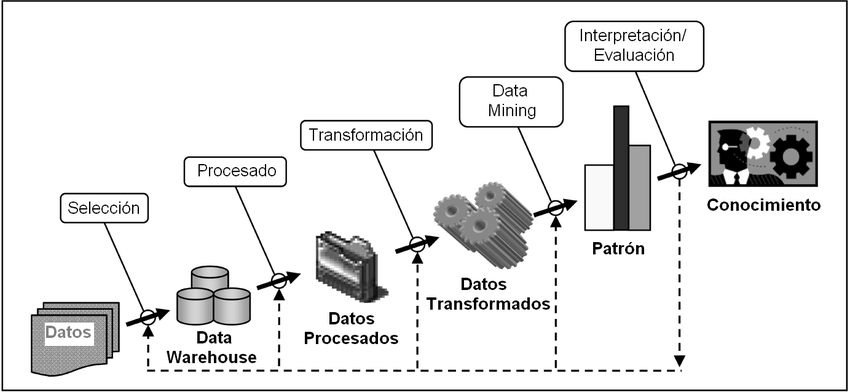
\includegraphics[width=0.8\textwidth]{The-Steps-of-a-KDD-process.png}
    \caption{\label{fig:KDD} Proceso KDD} Fuente: \cite{fayyad1996kdd}.
\end{figure}
    
    A continuación, se describen con un poco más de detalle cada una de las seis etapas de Crisp-DM \cite{wirth2000crisp}:
\begin{enumerate}
    \item \textbf{Comprensión del negocio}: el objetivo principal es comprender los objetivos y requisitos del proyecto desde una perspectiva empresarial con el fin de convertirlos en objetivos técnicos y en un plan de Proyecto. Crisp-DM propone 4 tareas para completar esta etapa:
    \begin{itemize}
        \item Determinar objetivos del negocio
        \item Evaluar la situación actual
        \item Determinar los objetivos del proyecto de minería de datos.
    \end{itemize}
    \item \textbf{Comprensión de los datos}: tiene como objetivo principal tener el primer acercamiento con los datos por parte del equipo de minería de datos. Para esto es común que se realicen análisis exploratorio de datos, detección de \textit{missing values} y cualquier tipo de evaluación que pueda entregar hipótesis sobre el estado de los datos. Para esta etapa, se propone completar las siguientes tareas:
    \begin{itemize}
        \item Recolectar datos iniciales
        \item Describir los datos
        \item Explorar los datos
        \item Verificar la calidad de los datos
    \end{itemize}
    \item \textbf{Preparación de los datos}: la idea es preparar los datos para ser luego utilizados por alguna técnica de minería de datos en la etapa de modelado.  Crisp-DM propone seguir las siguientes tareas para poder lograr todo este cometido:
    \begin{itemize}
        \item Seleccionar datos
        \item Limpiar datos
        \item Estructurar datos
        \item Integrar datos
        \item Formatear datos
    \end{itemize}
    \item \textbf{Modelado}: en esta etapa se espera que los expertos en minería de datos elijan un modelo que pueda cumplir los requisitos del problema planteado en la etapa de comprensión del negocio. Una vez implementado el modelo, éste debe ser evaluado y analizado por los expertos  en minería de datos con el fin de poder ajustarlo en base a los datos que se poseen dentro de la compañía. En particular se proponen las siguientes tareas para la realización de esta etapa:
    \begin{itemize}
        \item Seleccionar la técnica de modelado
        \item Generar métodos de evaluación del modelo
        \item Construir el modelo
        \item Evaluar el modelo
    \end{itemize}
    \item \textbf{Evaluación}: Acá los expertos en el dominio analizan y evalúan los resultados del modelo producido en la etapa anterior. Esto se realiza teniendo en cuenta los criterios de éxito del problema definidos en la etapa número 1 como modo de validación del modelo empleado en la etapa número 4. Como en cada una de las etapas Crisp-DM propone subtareas asociadas a la etapa de evaluación, las cuales pasamos a definir a continuación:
    \begin{itemize}
        \item Evaluar los resultados
        \item Revisar del proceso
        \item Determinar los próximos pasos
    \end{itemize}
    \item \textbf{Implantación}: una vez que el modelo ha sido construido y validado, llega la hora de desplegar la solución generada. Para realizar esto, y dependiendo de la particularidad de cada proyecto, se pueden tomar acciones dentro del proceso de negocio que van desde recomendaciones del analista basadas en la observación y resultados del modelo. En general para realizar esto de buena manera, Crisp-DM recomienda cumplir las siguientes entregas: 
    \begin{itemize}
        \item Plan de implantación
        \item Plan de monitoreo y mantención
        \item Informe final
        \item Revisión del proyecto
    \end{itemize}
\end{enumerate}
    
\subsubsection{Framework para Minería de textos según Dasri}
    \cite{dasritext} propone un \textit{framework} para desarrollar proyectos de minería de textos, el cual se puede resumir en tres pasos (Ver figura \ref{fig:Framework_TM} ): Preprocesamiento de textos, Aplicación de técnicas de minería de textos y Análisis de textos. A continuación se describen cada una de las etapas:
    \begin{enumerate}
        \item \textbf{Preprocesamiento de textos}: en general antes de aplicar cualquier técnica de minería de textos se deben realizar un par de tareas de preprocesamiento con el fin de obtener información más certera en la siguiente etapa del proyecto de minería de textos. Las tareas más recurrentes de preprocesamiento de textos son:
        \begin{itemize}
            \item Tokenización: un documento es una colección de oraciones. En este paso se busca dividir la totalidad de las oraciones en su unidad más básica, es decir palabras. Para lograr esto se eliminan puntos , comas y espacios en blanco.
            \item Eliminación de \textit{StopWords}: en este paso se busca eliminar todos los \textit{tokens} obtenidos en el paso anterior que se identifiquen como \textit{stopwords}. Se conoce como \textit{stopwords} a las palabras que tienen una pequeña o ninguna significancia por si solas. En general cada idioma tiene una lista predeterminada de \textit{stopwords} por ejemplo en inglés los más conocidos son: 'a’, 'is’, 'of’, 'an’, etc.
            \item Stemming: es la tarea de identificar la raíz de ciertas palabras. En la figura \ref{fig:Stemming} se puede apreciar como las palabras ``Jumps'', ``Jumped'' y ``Jumping'' fueron sometidas al proceso de Stemming cuyo resultado final fue ``Jump''.
        \end{itemize}
    \item \textbf{Técnicas usadas en minería de textos}: en esta etapa dependiendo del objetivo del proyecto de minería de textos se pueden utilizar técnicas y algoritmos que cumplan alguna de las siguientes tareas:
        \begin{itemize}
            \item Extracción de información
            \item Categorización
            \item \textit{Clustering} de textos
            \item Visualización de textos
            \item Resumen de textos
        \end{itemize}
    \item \textbf{Análisis de textos}: en esta etapa se deben interpretar los resultados obtenidos luego de aplicar las técnicas de minería de textos, para así, poder extraer los patrones y el conocimiento implícito en el \textit{corpus} estudiado. Todo esto debe ser plasmado en un documento, que nos deberá mostrar los resultados finales del proyecto.
    \end{enumerate}
\begin{figure}[H]
    \centering
    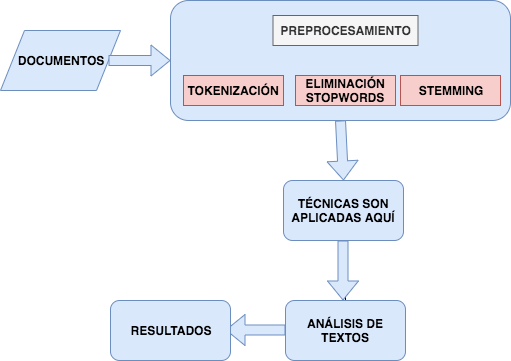
\includegraphics[width=0.8\textwidth]{Framework_TM.png}
    \caption{\label{fig:Framework_TM} \textit{Framework} para minería de textos según Dasri} Fuente: Text Mining Framework, Methods and Techniques \cite{dasritext}
\end{figure}

\begin{figure}[H]
    \centering
    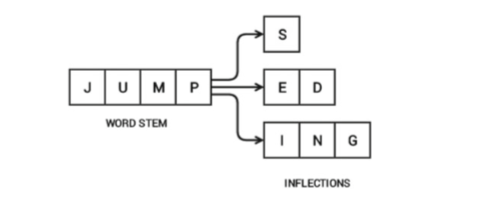
\includegraphics[width=0.8\textwidth]{figures/Stemming.png}
    \caption{\label{fig:Stemming} Proceso de \textit{Stemming}} Fuente: Text Analytics with Python \cite{sarkar2016text}
\end{figure}

    Una vez finalizadas las dos etapas del proceso de minería de textos, se deben interpretar las salidas de los algoritmos empleados en la etapa de aplicación de técnicas para así poder extraer los patrones y el conocimiento implícito en los documentos. Todo esto debe ser plasmado en un documento que nos deberá mostrar los resultados finales del proyecto.
    
\subsubsection{\textit{Framework} para en minería de textos según Kumar}
    \cite{kumar2014survey} propone un \textit{framework} para proyectos en minería de textos un poco más detallado que el descrito en la sección anterior. La metodología se compone en cinco etapas (ver figura \ref{fig:Framework_Ku}). A continuación se pasa a describir las etapas propuestas por Kumar una por una:
    \begin{enumerate}
        \item \textbf{Preprocesamiento de textos}: al igual que en el marco de trabajo propuesto por Dasri, antes de realizar cualquier trabajo con los documentos éstos deben ser preprocesados. Para realizar esto se proponen las mismas tres etapas que proponía Dasri:
        \begin{enumerate}
            \item Tokenización
            \item Eliminación de \textit{stopwords}
            \item \textit{Stemming}
        \end{enumerate}
        \item \textbf{Transformación de textos}: se debe buscar una representación matemática para los textos que se están trabajando. En general existen dos posibles formas de representar textos de forma matemática: Bolsas de palabras o Vectores de Secuencia. Cada uno de estos métodos generan los \textit{features}, que posteriormente, serán consumidos por algún algoritmo de minería de textos.
        
        \item \textbf{Selección de características}: en esta fase se busca disminuir la cantidad de \textit{features} generadas en el proceso anterior. Para esto se busca eliminar las características consideradas como irrelevantes para los procesos de minería de textos. Una vez finalizada esta etapa, el tamaño del \textit{dataset} a utilizar debería ser mucho más pequeño que al comienzo de la etapa, lo que implicará menores costos computacionales y espacio de búsqueda.
        \item \textbf{Aplicación de técnicas usadas en minería de textos}: En esta etapa Kumar propone lo mismo que Dasri, es decir  dependiendo de nuestro objetivo debemos seleccionar la técnica de minería de textos que cumpla alguna de las tareas comunes de la disciplina.

        \item \textbf{Evaluación de resultados}: tras la etapa anterior se deben analizar e interpretar los resultados. Además es vital utilizar métricas para evaluar el rendimiento de nuestros algoritmos como porcentajes de \textit{accuracy}, precisión, entre otras métricas útiles dependiendo de la técnica empleada.
    \end{enumerate}
    \begin{figure}[H]
    \centering
    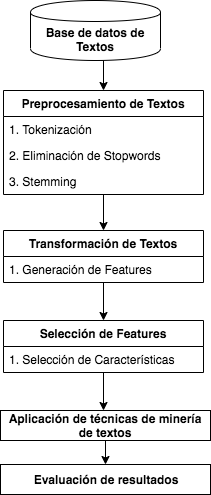
\includegraphics[height=0.7\textheight,width=0.5\textwidth]{figures/Framework_Kumar.png}
    \caption{\label{fig:Framework_Ku} Framework para minería de textos según Kumar} Fuente: A survey on text mining process and techniques \cite{kumar2014survey}
\end{figure}  

\subsubsection{Guía para proyectos de clasificación de Textos según Google}
    \cite{Google} propone un esquema de trabajo para enfrentar problemas de clasificación de textos de una forma un poco más técnica que los otros frameworks  estudiados hasta ahora. En esta guía, Google propone el siguiente flujo de trabajo (ver figura \ref{fig:Workflow_Google}) para un proyecto de clasificación de textos.
    \begin{figure}[h]
        \centering
        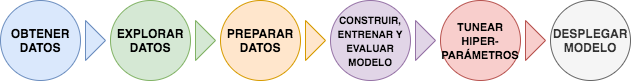
\includegraphics[width=0.8\textwidth]{figures/Workflow_Google.png}
        \caption{\label{fig:Workflow_Google} Flujo de trabajo para problemas de clasificación de textos según Google} Fuente: Text Clasification, Google Developers \cite{Google}
    \end{figure}
    A continuación, se describen cada una de las etapas del flujo de trabajo propuesto por Google:
    \begin{enumerate}
        \item \textbf{Obtener Datos}: para empezar, lo primero que se debe tener son textos. Según Google, los resultados de un proyecto de clasificación de textos dependen mucho de la calidad de los textos que se utilicen para entrenar cualquier tipo de modelo, por lo que este paso resulta vital.  En este caso Google indica que existen diversas fuentes para obtener textos tales como \textit{APIs} de diversas compañías o incluso los propios textos que pueda tener la compañía patrocinadora del proyecto. En cualquiera de los casos anteriores Google indica que se deben tener las siguientes consideraciones a la hora de recolectar datos:
        \begin{itemize}
            \item intentar recolectar la mayor cantidad de textos para entrenar el modelo, ya que esto ayudará a generalizar de mejor forma los resultados.
            \item asegurar tener un \textit{dataset} balanceado, es decir intentar tener la misma cantidad de datos para cada clase a clasificar.
            \item intentar tener datos que cubran todos los casos posibles y no sólo usar con los casos comunes. 
        \end{itemize}
       \item \textbf{Explorar Datos}: una vez construido u obtenido un \textit{dataset}, es sumamente importante revisar que éste sea consistente con las expectativas del proyecto. Para realizar esto, se deben realizar revisiones aleatorios a los datos y ver, por ejemplo, si las etiquetas de éstos corresponden a lo que se espera.
       Otra cosa relevante que se propone en esta guía es la revisión de ciertas métricas que permitirán determinar si el \textit{dataset} es apto para ser utilizado en un problema de clasificación de textos:
       \begin{itemize}
           \item Número de muestras
           \item Número de clases
           \item Número de clases por muestras
           \item Número de palabras por muestras
           \item Distribución de palabras según frecuencia
           \item Distribución de muestras según largo
       \end{itemize}   
      \item \textbf{Elección de un modelo}: una de las cosas más importantes a la hora de seleccionar un modelo de clasificación es resolver el \textit{trade-off} entre \textit{accuracy} y tiempo de cómputo. Para esto, Google desarrolló un algoritmo para seleccionar un modelo de clasificación de textos, el cual permite dependiendo del \textit{dataset}, seleccionar el modelo que permita encontrar el mayor \textit{accuracy} en el menor tiempo posible. 

    \item \textbf{Prepararación de datos}: Tras la etapa anterior, es necesario llevar los datos a alguna representación numérica dependiendo del algoritmo a utilizar. Para realizar esto existen dos alternativas:
    \begin{itemize}
        \item Tokenización: dividir los textos en palabras u oraciones. Esto permitirá generalizar la relación entre los textos y las etiquetas asociadas a cada uno. 
        \item Vectorización: definir una buena medida numérica para caracterizar los textos.
    \end{itemize}
        En general, Google propone técnicas de tokenización en el caso de utilizar algoritmos basados en n-gramas. Por otro lado si se desean utilizar algoritmos secuenciales se sugiere utilizar técnicas de vectorización para representar los textos. 
        
        Una vez representados los datos de forma numérica se debe emplear alguna técnica de selección de características; para el caso particular de textos, Google propone utilizar las funciones de clasificación F y Chi Cuadrado.
    \item \textbf{Construir, entrenar y evaluar el modelo}: en esta etapa, Google propone formas y matices para construir, entrenar y evaluar el desempeño de una red neuronal con perceptrones multicapa y de una red neuronal recurrrente. 
    \item \textbf{Desplegar modelo}: esta etapa da algunos consejos con el fin de tener un buen rendimiento en producción del modelo generado una vez terminado el proyecto. A continuación, se describen los principales consejos descritos por Google:
    \begin{itemize}
        \item Se debe asegurar que los datos que serán evaluados con el modelo construido siguen la misma distribución que los datos usados para entrenar y validar el modelo.
        \item Regularmente se debe re-evaluar el modelo con nuevos datos adquiridos.
        \item Si la distribución de datos cambia, se debe reentrenar el modelo.
    \end{itemize}
    \end{enumerate}
    
\subsubsection{Comparación de metodologías de minería de textos}
    A continuación, se realizará una comparación entre las metodologías descritas en las secciones anteriores, con el fin de tener una visión general de qué es lo que ofrece cada una. Para ello, se contruyó una tabla (Ver tabla \ref{table:comparación_metodologías_tm}), en donde, las filas representan a etapas mencionadas dentro de la metodología, mientras que las columnas representan a una metodología en específico. El color achurado en la tabla indica si la metología, de la fila, menciona a la etapa, de la columna, como parte del proceso de minería de textos. En caso de que la metodología no presente a la etapa dentro del proceso descrito, se dejó el espacio en blanco dentro de la tabla.
    
    Si se analiza la tabla \ref{table:comparación_metodologías_tm}, se puede ver que las metodologías que realizan un desglose más detallado de las tareas generales de un proyecto de minería de textos son las propuestas por Kumar y la propuesta por Google, siendo está última la que más detalles entrega en cómo enfrentar cada uno de los problemas, esto ocurre debido a que Google propone una guía por sobre una metodología. Por otro lado la metodología propuesta por Dasri salta varios pasos fundamentales para poder terminar con éxito un proyecto de minería de textos.

    \begin{table}[H]
    \centering
    \begin{tabular}{c|c|c|c|}
    \cline{2-4}
                                                       & Kumar                    & Dasri                    & Google                   \\ \hline
    \multicolumn{1}{|c|}{Preprocesamiento}             & \cellcolor[HTML]{DAE8FC} & \cellcolor[HTML]{DAE8FC} & \cellcolor[HTML]{DAE8FC} \\ \hline
    \multicolumn{1}{|c|}{Transformación}               & \cellcolor[HTML]{DAE8FC} &                          & \cellcolor[HTML]{DAE8FC} \\ \hline
    \multicolumn{1}{|c|}{Selección de Características} & \cellcolor[HTML]{DAE8FC} &                          & \cellcolor[HTML]{DAE8FC} \\ \hline
    \multicolumn{1}{|c|}{Aplicación de Modelo}         & \cellcolor[HTML]{DAE8FC} & \cellcolor[HTML]{DAE8FC} & \cellcolor[HTML]{DAE8FC} \\ \hline
    \multicolumn{1}{|c|}{Evaluación de Modelo}         & \cellcolor[HTML]{DAE8FC} & \cellcolor[HTML]{DAE8FC} & \cellcolor[HTML]{DAE8FC} \\ \hline
    \end{tabular}
    \caption{\label{table:comparación_metodologías_tm} Tabla comparativa metodologías en minería de texto.} Fuente: Elaboración Propia.
    \end{table}
    
\subsection{Preprocesamiento de textos}
    En general, cuando se desea analizar textos, es esperable que se pruebe algún algoritmo de minería de textos, cuyas entradas, en su mayoría, son elementos numéricos. Sin embargo, antes de poder realizar la transformación de textos a números, es necesario realizar algunos ajustes a los textos, pues los textos por naturaleza son datos no estructurados y poco estandarizados. En general, las técnicas de preprocesamiento buscan generar secuencias de componentes lingüísticos con una estructura y notación estándar, para así poder conseguir buenos resultados con alguna técnica en particular.
    
    En esta sección se describen las principales tareas y técnicas utilizadas a la hora de preprocesar textos. Para ello se utilizará el siguiente texto de ejemplo '' Nosotros discutimos brevemente sobre la sintaxis, estructura y diseño de filosofías.``    
\subsubsection{Tokenización de textos}
    Antes de poder hablar de tokenización de textos, es necesario definir que es un \textit{token}. Se entiende por \textit{token} a componentes independientes y mínimos textuales que por si sólos tienen una definida síntaxis y semántica \cite{sarkar2016text}. En general, se puede considerar como un \textit{token} a las oraciones que componen un párrafo o incluso a las palabras que componen una oración. 
    
    Ahora teniendo en cuenta qué es un token, se puede definir a la tokenización de textos como el proceso de romper un documento en sus respectivos \textit{tokens}, ya sean oraciones o palabras. A continuación, se utiliza el texto de ejemplo, definido anteriormente, para que quede claro el proceso de tokenización.
    
    
    \begin{table}[H]
    \centering
    \begin{tabular}{|c|c|}
    \hline
    \textbf{Texto en bruto}                                                                                                                & \textbf{Texto tokenizado}                                                                                                                                                                 \\ \hline
    \begin{tabular}[c]{@{}c@{}}``Nosotros discutimos brevemente \\ sobre la sintaxis, estructura \\ y diseño de filosofías.''\end{tabular} & \begin{tabular}[c]{@{}c@{}}[``Nosotros'', ``discutimos'', ``brevemente''\\  ``sobre'' ,``la'', ``sintaxis'',``estructura'' , ``y'', ``diseño'',\\  ``de'',  ``filosofías.'']\end{tabular} \\ \hline
    \end{tabular}
\end{table}

\subsubsection{Eliminación de caracteres especiales}
    Una tarea importante en el proceso de normalización de textos, es la eliminación de caracteres innecesarios y especiales. Estos pueden ser símbolos de exclamación, interrogación, puntuación e incluso etiquetas HTML en el caso de estar trabajando con datos extraídos directamente desde una página web. La principal razón de realizar este proceso es que a menudo estos caracteres no entregan mucha significancia cuando analizamos los textos utilizando técnicas de minería de textos o procesamiento de lenguaje natural.
    
    A continuación, se utiliza el texto de ejemplo para comprender el proceso de eliminación:
    
    \begin{table}[H]
    \centering
    \begin{tabular}{|c|c|}
    \hline
    \textbf{Texto tokenizado}                                                                                                                                                                     & \textbf{Texto sin caracteres especiales}                                                                                                                                                     \\ \hline
    \begin{tabular}[c]{@{}c@{}}[``Nosotros'', ``discutimos'', ``brevemente'', \\ ``sobre'' , ``la'', ``sintaxis'', \\ ``estructura'' , ``y'', ``diseño'', \\ ``de'',``filosofías.'']\end{tabular} & \begin{tabular}[c]{@{}c@{}}[``Nosotros'', ``discutimos'', ``brevemente'',\\  ``sobre'' , ``la'', ``sintaxis'', \\ ``estructura'' , ``y'',\\  ``diseño'', ``de'',``filosofías'']\end{tabular} \\ \hline
    \end{tabular}
    \end{table}
    
    Como se puede apreciar, el último token, ''filosofías.`` tenía un punto al final. Es por ello, que luego del proceso de eliminación de caracteres especiales, dicho punto fue eliminado.
    
\subsubsection{Eliminación de stopwords}
    El proceso de eliminación de \textit{stopwords} es uno de los principales de la normalización de textos. Se define un \textit{stopword} como aquellas palabras que prácticamente no poseen significado o utilidad por si solas. Algunos ejemplos de \textit{stopwords} son preprocisiones, pronombres, artículos e incluso algunos adverbios en español \cite{sarkar2016text}. 
    
    A continuación, se toma el conjunto de palabras que obtuvimos en la sección anterior y se aplica el proceso de eliminación de \textit{stopwords}, con el fin de ver cómo disminuye el número de tokens a trabajar, una vez efectuado este simple procedimiento:
    
    \begin{table}[H]
    \centering
    \begin{tabular}{|c|c|}
    \hline
    \textbf{\begin{tabular}[c]{@{}c@{}}Texto tokenizado,\\ sin caracteres especiales\end{tabular}}                                                                                               & \textbf{Texto sin stopwords}                                                                                                                                          \\ \hline
    \begin{tabular}[c]{@{}c@{}}[``Nosotros'', ``discutimos'', ``brevemente'', \\ ``sobre'' , ``la'', ``sintaxis'', \\ ``estructura'' , ``y'', ``diseño'', \\ ``de'',``filosofías'']\end{tabular} & \begin{tabular}[c]{@{}c@{}}[``Nosotros'', ``discutimos'', ``brevemente'',\\  ``sobre'' , ``sintaxis'', \\ ``estructura'' ,\\  ``diseño'',``filosofías'']\end{tabular} \\ \hline
    \end{tabular}
    \end{table}

    Una vez realizada la eliminación de \textit{stopwords} y la eliminación de caracteres especiales se logró disminuir el número de \textit{tokens} del texto original de 11 a 8. Osea que practicamente el 30\% de los \textit{tokens} no aportaban nada a posteriores análisis.

\subsubsection{Stemming}
    Para comprender el trabajo de \textit{stemming}, primero se debe entender que una palabra en cualquier lenguaje es regularmente compuesta por su forma básica (\textit{stem}) más un afijo. Los afijos son unidades como los prefijos y sufijos cuya finalidad es unirlos a palabras en su forma \textit{stem} para cambiar su signficado \cite{sarkar2016text}. En la figura \ref{fig:Stemming} se puede ver como el \textit{stem} \textit{jump} puede ser cambiado a distintas formas agregandos diferentes afijos.
    
    A continuación, se utiliza la misma lista de \textit{tokens} que se obtuvo en la sección anterior, esta vez, transformándolos todos a su forma básica.
    
    \begin{table}[H]
    \centering
\begin{tabular}{|c|c|}
\hline
\textbf{Texto tokenizado}                                                                                                                                           & \textbf{Texto en stem}                                                                                                                                 \\ \hline
\begin{tabular}[c]{@{}c@{}}[``Nosotros'', ``discutimos'', ``brevemente'', \\ ``sobre'' , ``sintaxis'', \\ ``estructura'' , ``diseño'',,``filosofías'']\end{tabular} & \begin{tabular}[c]{@{}c@{}}[``Nosotr'', ``discut'', ``brevement'', \\ ``sobr'' , ``sintaxis'', ``estructur'' , \\ ``diseñ'',,``filosof'']\end{tabular} \\ \hline
\end{tabular}
\end{table}
    
    Como se puede apreciar, el principal problema del proceso de Stemming, es que las palabras resultantes no existen necesariamente en el diccionario. Esto implica que, a la hora de realizar análisis, es probable que  los resultados no sean fáciles de interpretar ni comunicar.
    
\subsubsection{Lematización}
    El trabajo de \textit{lematización} es similar al proceso de \textit{stemming} con la diferencia que las palabras resultantes siempre estarán en el diccionario \cite{sarkar2016text}. El resultado del proceso de lematización de una palabra se conoce como el lema de ésta.  
    
    \begin{table}[H]
    \centering
\begin{tabular}{|c|c|}
\hline
\textbf{Texto tokenizado}                                                                                                                                           & \textbf{Texto en lema}                                                                                                                                     \\ \hline
\begin{tabular}[c]{@{}c@{}}[``Nosotros'', ``discutimos'', ``brevemente'', \\ ``sobre'' , ``sintaxis'', \\ ``estructura'' , ``diseño'',,``filosofías'']\end{tabular} & \begin{tabular}[c]{@{}c@{}}[``Nosotros'', ``discutir'', ``breve'', \\ ``sobre'' , ``sintaxis'', ``estructura'' , \\ ``diseño'',``filosofía'']\end{tabular} \\ \hline
\end{tabular}
\end{table}

    En general, dentro de las librerías existentes para lematizar, se debe indicar qué tipo de palabra se lematizará. Esto hace el trabajo un poco más complicado, ya que previo a poder lematizar \textit{tokens}, éstos deben estar etiquetados según su función en el contexto de la oración. Para solucionar esto, a continuación se describe la tarea Part of Speech (POS), la cual ayudará a solucionar este problema.
    
\subsubsection{Part of Speech}
    Part of Speech (POS) son categorías léxicas específicas a las cuales diversas palabras son asignadas acorde a su contexto sintáctico y rol dentro de un texto. Por ejemplo en inglés dependiendo del contexto la palabra ``Building'' puede ser un sustantivo o un verbo. 
    Los principales POS con que un \textit{token} puede ser etiquetado dentro de un texto son verbo, sustantivo, adjetivo o adverbio en su infinidad de combinaciones. En la tabla \ref{table:Etiquetas_POS} se puede revisar las distintas etiquetas que se le pueden aplicar a los distintas palabras de un documento.

\begin{table}[h!]
\centering
\begin{tabular}{|l|l|l|}
\hline
Number & Tag   & Description                              \\ \hline
1.     & CC    & Coordinating conjunction                 \\ \hline
2.     & CD    & Cardinal number                          \\ \hline
3.     & DT    & Determiner                               \\ \hline
4.     & EX    & Existential there                        \\ \hline
5.     & FW    & Foreign word                             \\ \hline
6.     & IN    & Preposition or subordinating conjunction \\ \hline
7.     & JJ    & Adjective                                \\ \hline
8.     & JJR   & Adjective, comparative                   \\ \hline
9.     & JJS   & Adjective, superlative                   \\ \hline
10.    & LS    & List item marker                         \\ \hline
11.    & MD    & Modal                                    \\ \hline
12.    & NN    & Noun, singular or mass                   \\ \hline
13.    & NNS   & Noun, plural                             \\ \hline
14.    & NNP   & Proper noun, singular                    \\ \hline
15.    & NNPS  & Proper noun, plural                      \\ \hline
16.    & PDT   & Predeterminer                            \\ \hline
17.    & POS   & Possessive ending                        \\ \hline
18.    & PRP   & Personal pronoun                         \\ \hline
19.    & PRP\$ & Possessive pronoun                       \\ \hline
20.    & RB    & Adverb                                   \\ \hline
21.    & RBR   & Adverb, comparative                      \\ \hline
22.    & RBS   & Adverb, superlative                      \\ \hline
23.    & RP    & Particle                                 \\ \hline
24.    & SYM   & Symbol                                   \\ \hline
25.    & TO    & to                                       \\ \hline
26.    & UH    & Interjection                             \\ \hline
27.    & VB    & Verb, base form                          \\ \hline
28.    & VBD   & Verb, past tense                         \\ \hline
29.    & VBG   & Verb, gerund or present participle       \\ \hline
30.    & VBN   & Verb, past participle                    \\ \hline
31.    & VBP   & Verb, non-3rd person singular present    \\ \hline
32.    & VBZ   & Verb, 3rd person singular present        \\ \hline
33.    & WDT   & Wh-determiner                            \\ \hline
34.    & WP    & Wh-pronoun                               \\ \hline
35.    & WP\$  & Possessive wh-pronoun                    \\ \hline
36.    & WRB   & Wh-adverb                                \\ \hline
\end{tabular}
\caption{\label{table:Etiquetas_POS} Etiquetas POS.} Fuente: Alphabetical list of part-of-speech tags used in the Penn Treebank Project:
\cite{POS_Tag}
\end{table}

\subsection{Transformación de textos}
    Una vez finalizado el preprocesamiento de textos, es necesario transformar los documentos en un formato entendible para los diversos modelos de minería de textos que se aplicarán en etapas posteriores. Para realizar esto, en general se ejecutan dos pasos:
    \begin{itemize}
        \item \textbf{Tokenización}: dividir el texto en palabras u oraciones. 
        \item \textbf{Vectorización}: definir una medida numérica para caracterizar cada token.
    \end{itemize}
    A continuación se describen dos métodos, que utilizando los pasos recién definidos, transforman los textos en elementos utilizables por algoritmos de minería de textos.
\subsubsection{Vectores de N-Gramas}
    En un vector de n-gramas, el texto es representado como una colección de únicos n-gramas. Se define a un n-grama como grupos de $n$ \textit{tokens} adyacentes. Por ejemplo en la oración \textit{``The mouse ran up the clock''} los n-gramas para $n=1$ son \textit{['the', 'mouse', 'ran', 'up', 'clock']}, para $n=2$ son \textit{['the mouse', 'mouse ran', 'ran up', 'up the', 'the clock']}.
    
    Una vez finalizado el proceso de construcción de n-gramas, se debe buscar la manera de representarlos numéricamente. Por lo general, la estrategia a seguir es utilizar alguna métrica que permita cuantificar el impacto de cierto n-grama en algún documento. Para esto existen algunas estrategias ya planteadas, las cuales se describen a continuación:
    \begin{itemize}
        \item \textbf{Codificación basada en frecuencias}: tal como dice el nombre, la estrategia a seguir en este tipo de vectorización es simplemente asignarle a cada uno de los n-gramas encontrados, la frecuencia absoluta que éste posee en el documento analizado.
        \item \textbf{Tf-idf}: es una técnica de vectorización extraída del campo de recuperación de la información. Esta técnica nace ya que por lo general existen ciertos n-gramas que aparecen con frecuencias absolutas muy parecidas entre distintos documentos. $Tf-idf$ es la multiplicación entre dos métricas importantes: frecuencias de términos y frecuencia inversa de documentos. A continuación se definen ambas métricas:
        \begin{enumerate}
            \item \textbf{Frecuencia de término}: es la frecuencia absoluta del término (n-grama) $i$ en el documento $j$. Se escribe como $tf$.
            \item \textbf{Frecuencia inversa en el documento}: Es la inversa de la frecuencia de documentos para cada término. Por lo que, se define a $idf$ como:
            \begin{equation*}
                idf(t) = 1+ log \left(\frac{C}{1+df(t)}\right)
            \end{equation*}
            Donde:
            \begin{itemize}
                \item $idf(t)$: Representa el $idf$ para el término $t$.
                \item $C$: Representa el número total de documentos en el corpus a analizar.
                \item $df(t)$: Representa el número de documentos en dónde el término $t$ aparece.
            \end{itemize}
    \end{enumerate}
    Como se mencionó anteriormente la métrica $tf-idf$ es la multiplicación de las dos métricas definidas anteriormente. Sin embargo a la hora de utilizarla se usa una versión normalizada, es decir, de la forma $\frac{tf-idf}{||tf-idf||}$.
   
    A modo de ejemplo, se calcularán vectores de un \textit{corpus} de documentos, basados en las dos estrategias definidas previamente. Para ello utilizaremos los siguientes textos: ``the sky is blue'', ``sky is blue and sky is beatiful'', ``the beautiful sky is so blue'' y ``i love blue cheese''.
    
    \begin{lstlisting}
    Usando frecuencia absoluta: 
   and  beautiful  blue  cheese  is  love  sky  so  the
0    0          0     1       0   1     0    1   0    1
1    1          1     1       0   2     0    2   0    0
2    0          1     1       0   1     0    1   1    1
3    0          0     1       1   0     1    0   0    0
    \end{lstlisting}
    \begin{lstlisting}
Usando tf-idf: 
        and  beautiful      blue    cheese        is      love       sky       so       the
0  0.000000   0.000000  0.399210  0.000000  0.488291  0.000000  0.488291  0.00000  0.603137
1  0.440516   0.347308  0.229880  0.000000  0.562351  0.000000  0.562351  0.00000  0.000000
2  0.000000   0.432026  0.285953  0.000000  0.349762  0.000000  0.349762  0.54797  0.432026
3  0.000000   0.000000  0.346182  0.663385  0.000000  0.663385  0.000000  0.00000  0.000000
    \end{lstlisting}
    Cada una de las filas de las matrices mostradas anteriormente representan un documento del \textit{corpus}, mientras que las columnas representan un n-grama presentes en el \textit{corpus} de documentos.  
    \end{itemize}
\subsection{Técnicas de minería y análisis de textos}
    Una vez finalizadas las etapas de preprocesamiento y transformación de textos, llega la hora de comenzar a extraer información de los datos en estudio. Para lograrlo existen varias tareas predefinidas en la literatura y más aún diversas técnicas que permiten resolverlas. A continuación se describirán algunas de las tareas más relevantes para el objetivo de esta memoria y las principales formas de resolverlas.
\subsubsection{Extracción de keywords en documentos utilizando n-gramas}
    Uno de los objetivos más importantes que se tienen a la hora de analizar textos es el de poder entender de qué habla el documento o el corpus a analizar. Para realizar esto, una de las formas más simples de hacerlo es encontrando las palabras o conceptos más relevantes dentro del documento. Para ser un poco más específico lo que se busca son los llamados  \textit{collocations}, un término traído desde el área lingüística el cual se puede definir como:  ``una secuencia o grupo de palabras que tienden a aparecer con frecuencia, tal que esta frecuencia es más que un hecho aleatorio'' \cite{sarkar2016text}. 
    
    Una forma de encontrar los \textit{collocations} más importantes de un documento en particular es utilizando n-gramas, ya definidos. Para esto se deben seguir dos pasos:
    \begin{enumerate}
        \item Encontrar los n-gramas 
        \item Rankear los n-gramas según algún criterio en particular
    \end{enumerate}
    El primer paso ya fue estudiado en extenso en la sección 2.4 por lo que ahora se procederá a explicar algunas métricas para rankear los n-gramas. La primera forma, y la más intuitiva quizás, para rankear los n-gramas es utilizando su frecuencia, es decir, se asume que los n-gramas que más aparecen en el documento serán los \textit{collocations} más importantes de éste. A continuación se presenta un pequeño texto, al cual le extraeremos los 5 bigramas con mayor frecuencia absoluta.
    
    \begin{lstlisting}[language=Bash]
    """
        Elephants are large mammals of the family Elephantidae
        and the order Proboscidea. Two species are traditionally recognised,
        the African elephant and the Asian elephant. Elephants are scattered
        throughout sub-Saharan Africa, South Asia, and Southeast Asia. Male
        African elephants are the largest extant terrestrial animals. All
        elephants have a long trunk used for many purposes,
        particularly breathing, lifting water and grasping objects. Their
        incisors grow into tusks, which can serve as weapons and as tools
        for moving objects and digging. Elephants' large ear flaps help
        to control their body temperature. Their pillar-like legs can
        carry their great weight. African elephants have larger ears
        and concave backs while Asian elephants have smaller ears
        and convex or level backs.
    """
    \end{lstlisting}
    Del texto anterior, los 5 bigramas con mayor frecuencia son:
    \begin{lstlisting}[language=Bash]
    [('african', 'elephants'), ('elephants', 'large'), ('africa', 'south'), ('african', 'elephant'), ('animals', 'elephants')]
    \end{lstlisting}
    
    De lo anterior se  puede inferir que el texto que se está analizando habla sobre elefantes del sur de África. Esto claramente es la idea más general del texto, y por ende nos entrega muy poca información. 
    
    Otra forma para rankear a los n-gramas encontrados es utilizando una medida llamada \textit{Información mutua puntual} (\textit{PMI} por sus siglas en inglés). El PMI puede ser calculado para dos \textit{tokens} como el logaritmo del cuociente entre la probabilidad de que ambos \textit{tokens} aparezcan en el documento y la multiplicación de las probabilidades individuales de cada \textit{token}, asumiendo que ambas probabilidades son independientes \cite{church1990word}. La expresión matemática que define esta medida es:
    \begin{equation*}
        pmi(x,y) = log\left(\frac{p(x,y)}{p(x)p(y)}\right)
    \end{equation*}
    
    Aplicando esta métrica al texto analizado anteriormente, obtenemos los siguientes 5 bigramas:
    
    \begin{lstlisting}[language=Bash]
    [('africa', 'south'), ('body', 'temperature'), ('breathing', 'lifting'), ('carry', 'great'), ('control', 'body'), ('convex', 'level'), ('ear', 'flaps'), ('elephantidae', 'order'), ('extant', 'terrestrial'), ('family', 'elephantidae')]
    \end{lstlisting}
    De aquí se puede apreciar que el texto habla sobre elefantes y sus principales características. Esto entrega un poco más de información que sólo rankear los \textit{collocations} encontrados utilizando su frecuencia absoluta.
    
\subsubsection{Técnicas para la extracción de temas a partir de documentos}
    Otra de las tareas más recurrentes en proyectos de minería de textos es el de modelamiento de temas. La tarea consiste en que a partir de un \textit{corpus} de documentos se deben descubrir los temas del cual éste habla. En general los temas se presentan como un conjunto de conceptos, que tienden a estar frecuentemente juntos. A continuación se describen algunos de los algoritmos más conocidos para cumplir esta tarea:
    \begin{itemize}
\item \textbf{Latent Dirichlet Allocation}: \cite{blei2003latent} (LDA por sus siglas) es un modelo generativo probabilístico que ayuda a encontrar los temas latentes que se encuentran dentro de un \textit{corpus} de documentos. Para realizar esto se asume que cada documento es una combinación de tópicos, los cuales siguen una distribución de Dirichlet. LDA recibe como parámetros un conjunto de documentos, el número $k$ de tópicos a encontrar y los parámetros de concentración $\alpha$ y $\beta$. Una vez procesados todos estos elementos el algoritmo retorna (Ver figura \ref{fig:LDA_Model}) los tópicos encontrados en el corpus y la distribución de tópicos para cada uno de los documentos estudiados. Estos dos elementos los pasaremos a definir a continuación:
    
    \begin{itemize}
        \item \textbf{Tópico}: es formado como una distribución de palabras, en donde cada palabra posee una probabilidad de pertenecer a dicho tópico.
        \item \textbf{Distribución de Tópicos}: un documento es formado como una distribución de tópicos, en donde cada tópico posee una probabilidad de pertenecer a dicho documento.
    \end{itemize}
    
    En la figura 6, se puede ver el algoritmo como una caja negra, en donde entra una cierta colección de documentos, se seleccionan ciertos parámetros $\alpha$ y $\beta$ para luego entregar tópicos y una distribución de tópicos para cada uno de los documentos analizados.
    
    \begin{figure}[h]
        \centering
        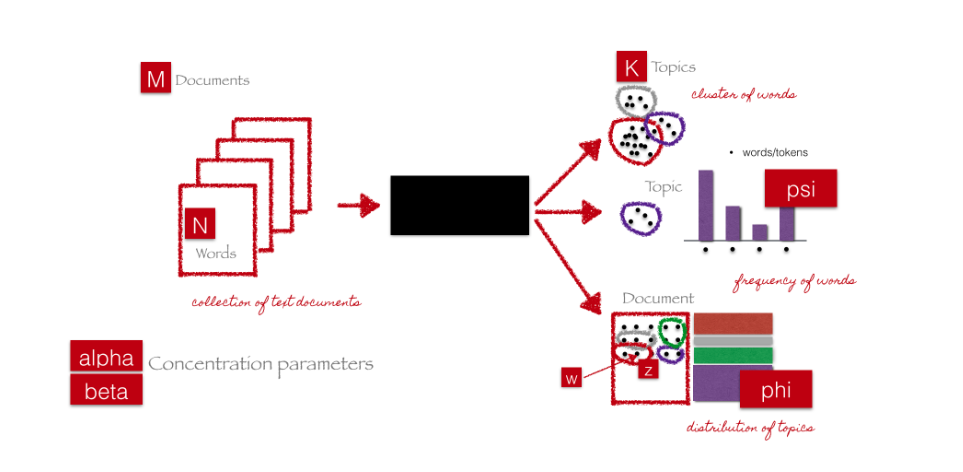
\includegraphics[width=1\textwidth]{figures/LDA.png}
        \caption{\label{fig:LDA_Model} Parámetros y Variables del Modelo} Fuente: Introduction to Topic Modeling in Python, PyGotham 2015 \cite{LDA_Model}
    \end{figure}
    
    Para realizar este trabajo LDA sigue el siguiente proceso iterativo:
    
    \begin{enumerate}
        \item Inicializa los parámetros $k$, $\alpha$ y $\beta$.
        \item Para cada documento, asigna aleatoriamente cada palabra a uno de los $k$ tópicos.
        \item Repetir los siguientes pasos hasta converger:
        \item Para cada documento $d$:
        \begin{enumerate}
            \item Para cada palabra $w$ en el documento:
            \begin{itemize}
                \item Para cada tópico $t$:
                \begin{itemize}
                    \item Calcular $P(t/d)$, la cual es la proporción de palabras en $d$ asignados al tópico $t$.
                    \item Calcular $P(w/t)$, la cual es la proporción de asignaciones al tópico $t$ sobre todos los documentos dada la palabra $w$.
                \end{itemize}
            \item Reasignar la palabra w con tópico t cuya probabilidad es $P(t/d) \cdot P(w/t)$ considerando todas las demas palabras y sus tópicos asignados.
            \end{itemize}
        \end{enumerate}
    \end{enumerate}
    
\item \textbf{Non-negative matrix factorization} (NNMF por sus siglas): es un algoritmo de factorización para matrices no negativas. Su principal diferencia con LDA es que es un algoritmo completamente determinista, o sea dada una serie de parámetros la sálida del algoritmo siempre es la misma. Formalmente se puede definir a NNMF como: Dada una matriz no negativa $V$, se deben encontrar dos matrices no negativas $W$ y $H$ las cuales multiplicadas aproximen V \cite{lee1999learning}. Matemáticamente esta representación es:
     
    \begin{equation*}
        V \approx WH
    \end{equation*} 
    Para obtener esta aproximación, usualmente se intenta disminuir alguna función de costo como la distancia euclídeana o la norma L2 entre las dos matrices, lo que es representado como:
    
    \begin{equation*}
        \text{argmin}_{\substack{W,H}} \frac{1}{2}||V-WH||^2
    \end{equation*}
    
    Si se considera la distancia euclideana como función de costo, lo anterior se resume a:
    
    \begin{equation*}
        \frac{1}{2}\sum_{i,j} \left( V_{ij} - WH_{ij} \right)^2 
    \end{equation*}
    
\item \textbf{Métricas para la evaluación de modelos:} 
    Una de las tareas más importantes a la hora de realizar modelamiento de tópicos, es seleccionar el número correcto de tópicos a encontrar. Para ello, existen algunas métricas que nos ayudan a evaluar la calidad de los tópicos encontrados. A continuación se definen algunas de estas métricas:
    \begin{enumerate}
        \item \textbf{Coherencia}: la coherencia de los tópicos encontrados por un algoritmo \cite{mimno2011optimizing}, indica qué tan coherentes son las palabras que se encuentran dentro de cada tópico. Para ello, se deben seleccionar las palabras más representativas dentro de cada tópico, y luego medir la ocurrencia y co-ocurrencia dentro del \textit{corpus} de documentos. La formulación matemática del índice de coherencia:
        \begin{equation*}
            Coherence(t) = \sum_{m=2}^M\sum_{i=1}^{m-1}\frac{\log{ D(w_m,w_t)+1}}{D(w_t)}
        \end{equation*}
        en donde:
        \begin{itemize}
            \item $M$ es la lista de las $M$ palabras más representativas del tópico t.
            \item $D(w_t)$ representa la ocurrencia de las palabra $w_t$ dentro del corpus.
            \item $D(w_m,w_t)$ la co-ocurrencia de la palabra $w_m$ y $w_t$ dentro del corpus.
        \end{itemize}
        \item \textbf{Coherencia CV}: la coherencia CV \cite{roder2015exploring}, es un índice que nos ayuda a cuantificar, qué tan interpretables por los humanos son los tópicos encontrados por algún algoritmo en particular. Su dominio se encuentra entre 0 y 1, siendo 1 la configuración ideal de tópicos para cierto \textit{corpus}.
    \end{enumerate}
\end{itemize}
     
\subsubsection{Algoritmos de clustering de documentos}
    Dentro de las familias de algoritmos en minería de textos se encuentran los algoritmos de \textit{clustering}, cuyo objetivo es N. Dentro de los algoritmos de \textit{clustering} existen al menos dos distintas categorías:
    \begin{itemize}
        \item \textbf{Clustering jerárquico}: este tipo de clustering se basa en el concepto que objetos similares son cercanos entre sí y lejanos a los objetos distintos en el espacio vectorial dónde son representados. Clusters son formados conectando objetos basados en su distancia y pueden ser visualizados usando un dendograma.
        
        \item \textbf{Clustering basado en centroides}: este tipo de clustering se construye de tal forma que cada cluster posee un centroide el cual es el miembro más representativo del cluster y además posee las características que distinguen el grupo encontrado del resto de los datos.
    \end{itemize}
    A continuación se describen los principales algoritmos de \textit{clustering} de cada una de las categorías descritas anteriormente.
\paragraph{Clustering jerárquico aglomerativo} 
\paragraph*{}Dentro del clustering jerárquico existen dos estrategias distintas para realizarlo:
    \begin{itemize}
        \item \textbf{Aglomerativo}: sigue una aproximación \textit{bottom-up}. Esto quiere decir que se comienza con todos los puntos en distintos \textit{clusters} y a medida que el algoritmo avanza se van uniendo hasta formar un único \textit{cluster} que contiene a todos los datos.
        \item \textbf{Divisivo}: al contrario del \textit{clustering} aglomerativo, sigue una aproximación top-down. Esto quiere decir, todos los puntos comienzan como un único \textit{cluster} y a medida que se avanza en el algoritmo, dichos \textit{clusters} son separados.
    \end{itemize}
    Para un \textit{clustering} de este tipo es necesaria la definición de dos métricas: Distancia entre puntos y criterio de enlace entre \textit{clusters}. Para ello se definen algunos de los criterios de enlace entre \textit{clusters} más utilizados en la literatura:
    
    Dados dos clusters, $P$ y $Q$ se definen los siguientes criterios de enlace:
    \begin{itemize}
        \item \textbf{Single Link}: 
        \begin{align*}
          d(P,Q) &= \min_{\substack{x \in P\\
                  y \in Q}}
        d(x,y) 
        \end{align*}
        \item \textbf{Complete Link}:
        \begin{align*}
          d(P,Q) = \max_{\substack{x \in P\\
                  y \in Q}}
        d(x,y) 
        \end{align*}
        \item \textbf{Group Average}:
        \begin{align*}
            d(P,Q) = \frac{1}{|P|\cdot|Q|} \sum_{\substack{x \in P\\
            y \in Q}}
            d(x,y)
        \end{align*}
        \item \textbf{Ward’s method}:
        \begin{align*}
            d(P,Q) &= \Delta SSE \\
            d(P,Q) &= \sum_{z \in P \cup Q} ||z-c_{P \cup Q}||^2- \left[\sum_{x \in P}||x-c_p||^2+\sum_{y \in Q}||y-c_q||^2\right] \\
            d(P,Q) &= \frac{|P|\cdot|Q|}{|P|+|Q|}||c_p-c_q||^2 
        \end{align*}
    \end{itemize}
    Utilizando alguno de dichos criterios de enlace más alguna medida de distancia se puede realizar un proceso de \textit{clustering} aglomerativo. 
    
    Algunas de las medidas de distancias más utilizadas en este tipo de algoritmos son:
    
    \begin{itemize}
        \item \textbf{Distancia Euclídeana}: o L2,  es definida como la distancia más corta que puede existir entre dos puntos. Matemáticamente se puede expresar como:
        \begin{equation*}
            d(p,q) = d(q,p) =\sqrt{\sum_{i=1}^n\left(q_i-p_i\right)^2}
        \end{equation*}
        \item \textbf{Distancia de Jensen Shannon}: propuesta como un método para medir la similitud entre dos distribuciones de probabilidad \cite{endres2003new}. Una definición de esta métrica es: Sean P y Q dos medidas de probabilidad, entonces se define la distancia de Jensen Shannon como:
        \begin{equation*}
        J(P,Q) = \frac{1}{2}\left(D(P||R)+D(Q||R)\right)
        \end{equation*}
        con $R=\frac{1}{2}(P+Q)$ y $D(\cdot||\cdot)$ es la divergencia Kullback-Leibler.
        \item \textbf{Distancia de Manhattan}: o L1, es definido como el camino más corto desde un punto $a$ a uno $b$ tomando solo rutas verticales u horizontales. Matemáticamente se expresa como:
        \begin{equation*}
            MD(u,v) = \sum_{i=1}^n \left|u_i - v_i\right|
        \end{equation*}
    \end{itemize}
    
\newpage    
    
\paragraph{Clustering basado en centroides}
\subparagraph{Algoritmo K-means}
\subparagraph*{}
    Uno de los algoritmos más famosos para realizar \textit{clustering} basado en centroides es el algoritmo K-means. K-Means tiene como entrada el número $k$ de clusters que deseamos encontrar y los datos.  Para entender mejor el algoritmo, enseguida se describe:
    \begin{lstlisting}
        Select k points as initial centroids.
        repeat
            Form k clusters by assigning each object to its closest centroid.
            Recompute the centroid of each cluster.
        until Centroids don't change or iterations.
    \end{lstlisting}
    Algunos elementos a considerar son:
    \begin{itemize}
        \item Los centroides iniciales son escogidos de forma aleatoria.
        \item El centroide de cada \textit{cluster} es la media aritmética de todos los elementos pertenecientes al mismo.
        \item La cercanía entre puntos es calculada usando la distancia euclideana.
    \end{itemize}
\paragraph{Métricas para la evaluación de clusters}
\paragraph*{}
    Para medir la calidad de los \textit{clusters} encontrados, existen dos grupos de métodos: intrínsecos y extrínsecos. Los primeros miden qué tan separados están los clústers entre sí. Por otro lado los métodos extrínsecos son utilizados cuando ya se conoce la agrupación de los datos que se tienen disponibles, es decir, sirven para probar algoritmos de clustering sobre datos donde ya se conoce la agrupación óptima. Para efectos de esta memoria, como no se conoce la configuración óptima de agrupaciones, se considerará sólo describir métodos íntrinsecos, siendo uno de ellos el coeficiente de Silhoutte.
    
    \begin{itemize} 
    \item \textbf{Coeficiente de Silhoutte}:
    Sea un \textit{dataset} $D$ de $n$ datos. Suponiendo que se generaron K \textit{Clusters}, $C_1,C_2,...,C_k$. Para cada dato $o \in D$, se calcula $a(o)$ como qué tan compacto está el clúster $C_i$ que contiene $o$  definido de la siguiente forma:
    
    \begin{equation*}
        a(o) = \frac{\sum_{o' \in C_i, o \neq o'}dist(o,o')}{|C_i| - 1 }
    \end{equation*}
    Luego se define $b(o)$, como el grado de separación, del dato $o$ respecto a los demás clusters.
    \begin{equation*}
        b(o) = \min_{C_j:1\leq j \leq k, j \neq i} \frac{\sum_{o' \in C_j}dist(o,o')}{|C_j|}
    \end{equation*}
    Finalmente se define el coeficiente de Silhouette \cite{rousseeuw1987silhouettes} como:
    \begin{equation*}
        s(o) = \frac{b(o) - a(o)}{max\{a(o),b(o)\}}
    \end{equation*}
    El coeficiente de Silhouette posee un dominio entre -1 y 1. Siendo 1 la configuración óptima, ya que asegura que un dato está bien cohesionado con su cluster y al mismo tiempo bien alejado de los otros clusters. Por otro lado, cuando el coeficiente de Silhoutte es -1 indica que el dato está cercano a otros \textit{clusters} y no bien cohesionado con su \textit{cluster}, por ende se tiene una mala configuración.
    
    El promedio del coeficiente de Silhoutte para todos los puntos dentro del \textit{dataset} a estudiar, indica qué tan buena es la configuración. Por lo que, se puede utilizar este índice para seleccionar el número adecuado de clusters a encontrar para cierto algoritmo. \end{itemize}

\subsubsection{Técnicas de visualización de textos}
    Una de las cosas más complejas que se debe realizar a la hora de ejecutar un proyecto de minería de textos es el de visualizar estos datos. Esto ocurre debido a que la mayoría de las herramientas de visualización trabajan con datos numéricos por lo que utilizar estas herramientas en el caso de textos no es algo tan natural. 
    
    Las técnicas de visualización de textos tienen muchas aplicaciones que van desde presentar resultados a los \textit{stakeholders} de nuestro proyecto de minería de textos hasta ser una herramienta de ayuda a la hora de seleccionar un modelo para trabajar sobre los datos.
    
    En las siguientes subsecciones, se describen algunas de las tareas más frecuentes a la hora de visualizar textos. Esto va, desde visualizar el comportamiento de ciertos conceptos en un documento particular hasta entender como varía dicho el uso de dicho concepto en un \textit{corpus}.

\paragraph{Análisis visual de características}
\paragraph*{}
    En proyectos de minería de datos es natural utilizar muchas técnicas de visualización para realizar tareas de selección de características, reducción de dimensionalidad e incluso encontrar patrones de forma visual. Dentro de estas técnicas en bajas dimensiones se encuentran visualizaciones tales como \emph{Pairwise Correlation HeatMaps y Barplots} que son utilizados para, por ejemplo, explicar la varianza de cada \textit{feature} y en lo posible encontrar correlaciones entre variables.
    
    Por otro lado en proyectos de minería de textos estas herramientas no son tan fáciles de utilizar por lo que se debe recurrir a otras técnicas para tener los primeros acercamientos con nuestros datos, tales como visualización de n-gramas, visualización de un temas y clustering de documentos.
    
\subparagraph{Visualización de N-Gramas}
\subparagraph*{}
    Como se revisó anteriormente una de las formas de representar un texto es utilizando n-gramas. Considerando que existen muchos n-gramas que se repiten a lo largo de un texto se pueden realizar diversas visualizaciones con esta agrupación de datos y su frecuencia.
\begin{enumerate}
    \item \textbf{Frecuencia de n-gramas a lo largo del tiempo}:
        considerando un \textit{corpus} de documentos y su fecha de emisión se puede construir una visualización que permita ver cómo ha variado la cantidad de menciones a cierto n-grama a lo largo del tiempo. A modo de ejemplo (ver figura \ref{fig:NgramasTiempo}), se puede ver cómo ha variado la cantidad de menciones sobre Donald Trump, Bernie Sanders y Hillary Clinton a lo largo del 2016. Para ello se tomó como corpus a estudiar los tweets emitidos en dicho año.
    \begin{figure}[H]
        \centering
        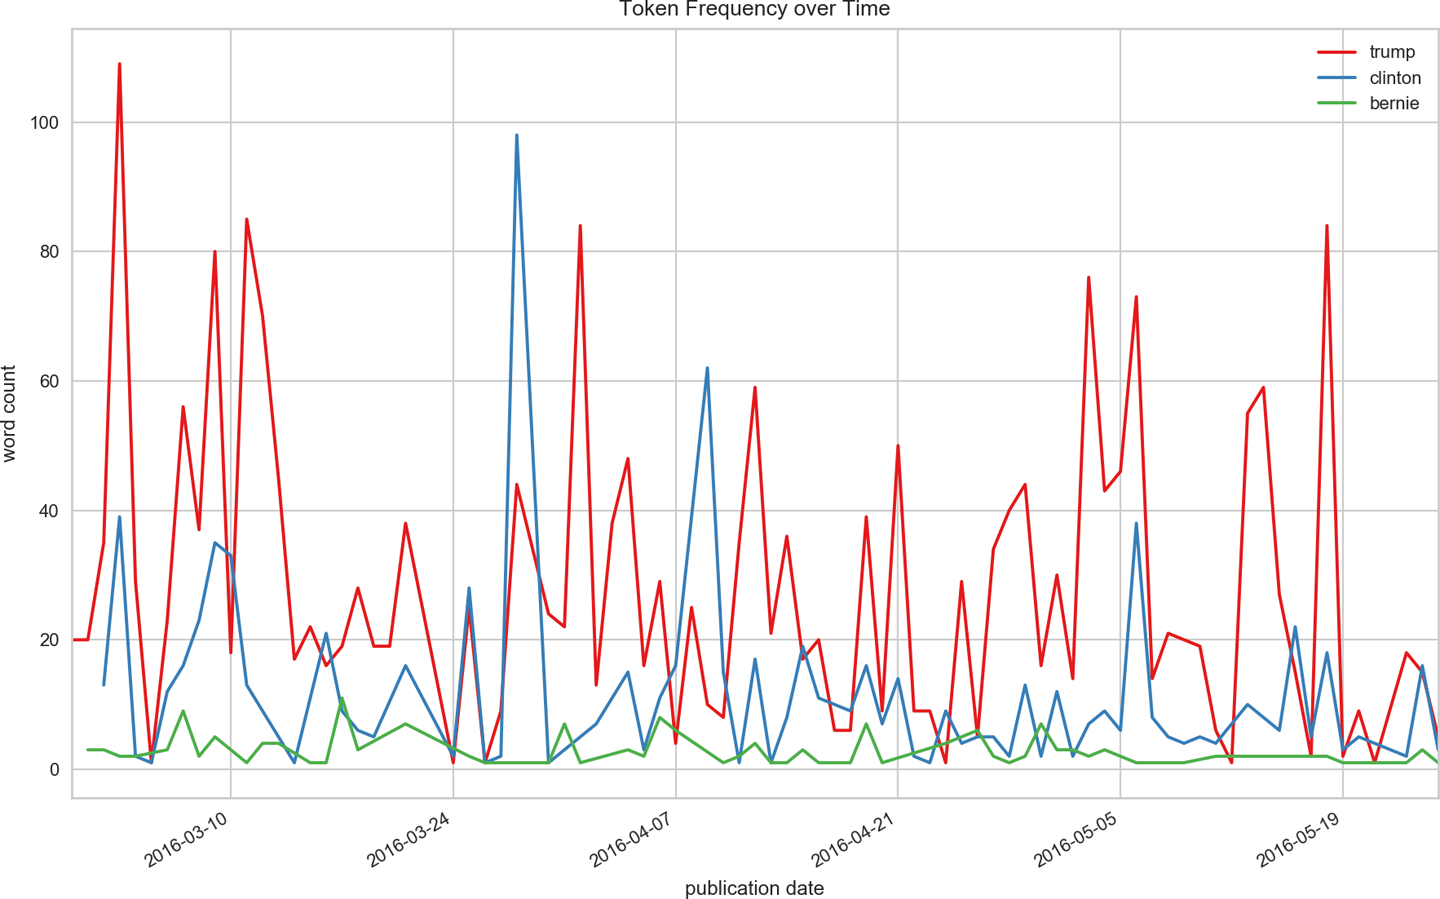
\includegraphics[width=0.8\textwidth]{figures/Frecuencia_sobre_tiempo.png}
        \caption{\label{fig:NgramasTiempo} Frecuencia de n-gramas a lo largo del tiempo} Fuente: Applied text analysis with python \cite{bengfort2018applied}
    \end{figure}
    \item \textbf{Dispersión léxica}: algo interesante que podemos visualizar dentro de un único documento es cómo los n-gramas más importantes aparecen y desaparecen. Para realizar esto se utilizan los gráficos de dispersión léxica (Ver figura \ref{fig:Lexical} ). A modo de ejemplo se puede ver como las palabras sobre conspiración que más utiliza Donald Trump en sus tweets han variado a lo largo de los años. Para ello en el eje Y, se listaron todas las palabras relacionados a conspiración. Luego en el eje X se listó la fecha de emisión de cada uno de los tweets estudiados, para finalmente, marcar con un punto los tweets que utilizaban dicho concepto.
    \begin{figure}[H]
        \centering
        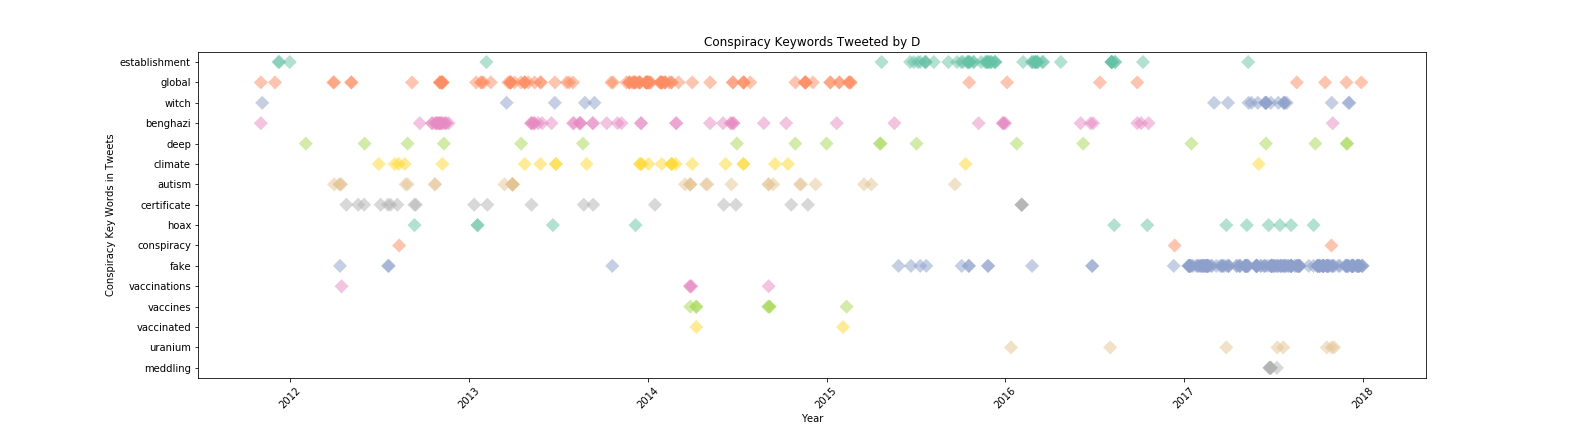
\includegraphics[width=1\textwidth]{figures/Lexical_Dispersion.png}
        \caption{\label{fig:Lexical}Dispersión Léxica de Tweets de Donald Trump} Fuente: Tutorial: Plotting Lexical Dispersion (Conspiracy Lies from the Left-of-Center) \cite{Lexical_Dispersion}
    \end{figure}
    
     En general dentro de los gráficos de dispersión léxica, el eje X puede ser un conjunto de documentos, tal como en el ejemplo recién estudiado, o un único documento en dónde el eje X pasaría a representar la temporalidad de dicho documento.
     
    \item \textbf{Distribución de frecuencias de n-gramas}:
        de la misma forma en que se pudo ver cómo varía la cantidad de menciones sobre un n-grama a lo largo del tiempo, también es posible ver cómo se distribuye la frecuencia de menciones de n-gramas en un documento particular. Para ello, simplemente se puede construir un gráfico de barras, en donde la altura de cada barra, representa la frecuencia de los n-gramas a analizar. A modo de ejemplo (Ver figura \ref{fig:DistribucionNgramas}), se puede ver la distribución de n-gramas de un documento en particular. Analizando esto, se puede ver que el texto habla sobre videojuegos debido a los conceptos que aparecen como más relevantes.
     \begin{figure}[h!]
        \centering
        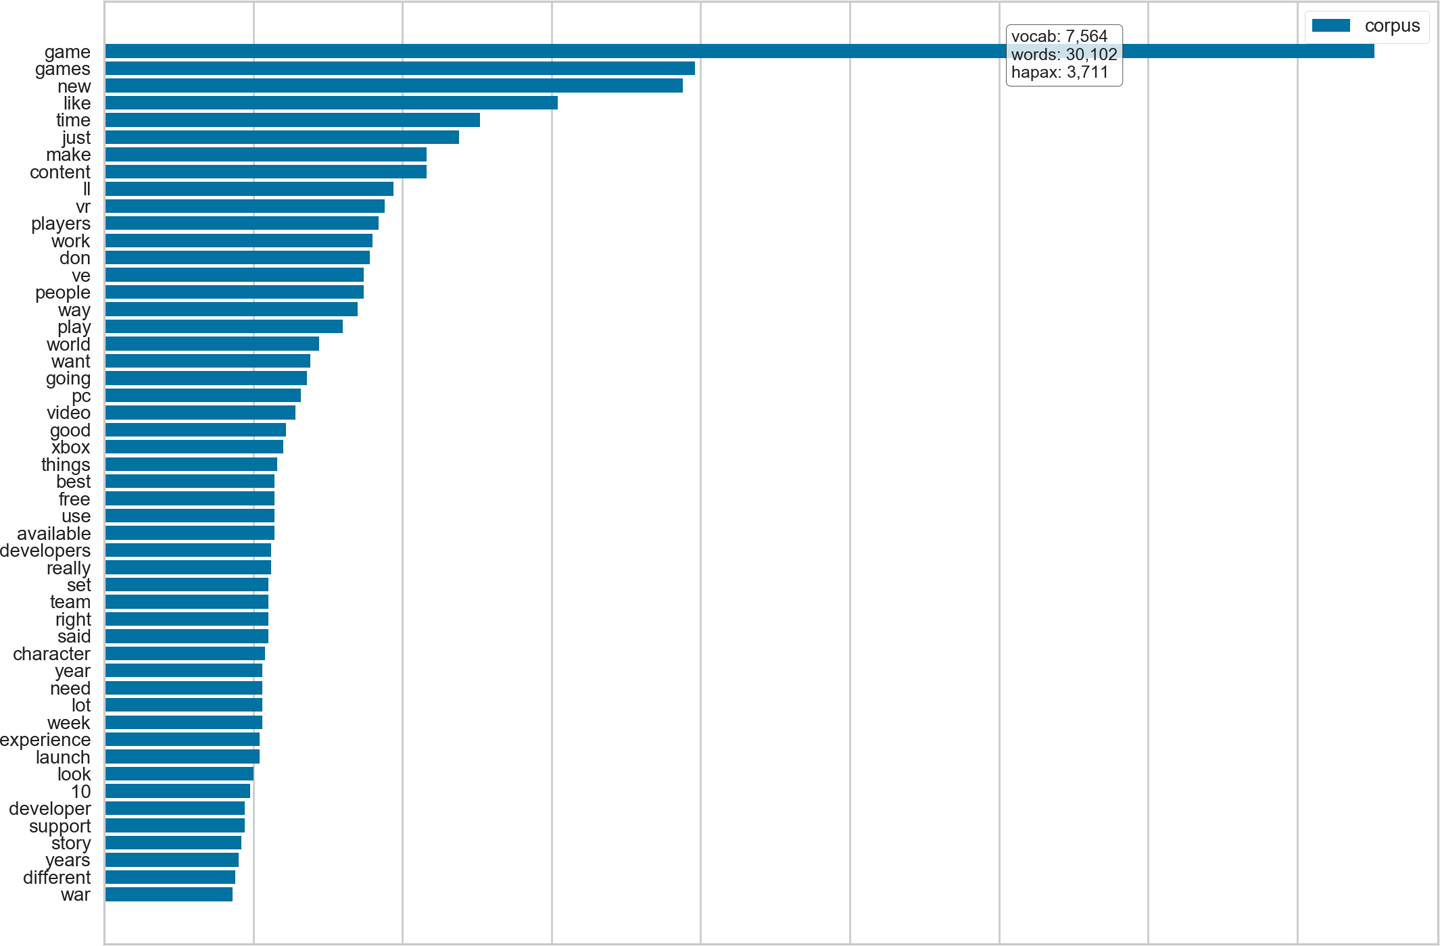
\includegraphics[width=0.8\textwidth]{figures/Distribucion.png}
        \caption{\label{fig:DistribucionNgramas} Distribución de frecuencia de n-gramas} Fuente: Applied text analysis with python \cite{bengfort2018applied}
    \end{figure}
    \item \textbf{Nube de Palabras}: otra forma de visualizar la frecuencia de las palabras es por medio del uso de nubes de palabras (ver figura \ref{fig:WordClouds}). Dentro de una nube de palabras se pueden ver los principales 1-gramas en distintos colores y tamaño. En general el tamaño es proporcional a la frecuencia de la palabra dentro del texto.
    \begin{figure}[H]
        \centering
        
\includegraphics[width=0.8\textwidth]{figures/Word-Cloud.png}
        \caption{\label{fig:WordClouds} Nube de Palabras} Fuente: Generating WordClouds in Python \cite{Word_Clouds}
    \end{figure}
\end{enumerate}
\subparagraph{Visualización  de entidades}
\subparagraph*{}
    Una de las tareas más comunes en proyectos de minería de textos es la identificación de las entidades nombradas dentro de un documento. A continuación se presentan algunas de las técnicas más comunes en este ámbito:
\begin{enumerate}
    \item Matriz de Co-Ocurrencias: indica de forma cualitativa cuántas veces coexisten dos entidades dentro de un mismo documento. A modo de ejemplo se puede ver la cantidad de co-ocurrencias entre los personajes del libro Mago de Oz (ver figrua \ref{fig:MatrizCoOcurrencias}). Además, como se puede apreciar se muestran dos matrices una ordenando los personajes por cantidad de menciones dentro de la obra y otra ordenando los personajes de forma cualitativa.  
    \begin{figure}[H]
        \centering
        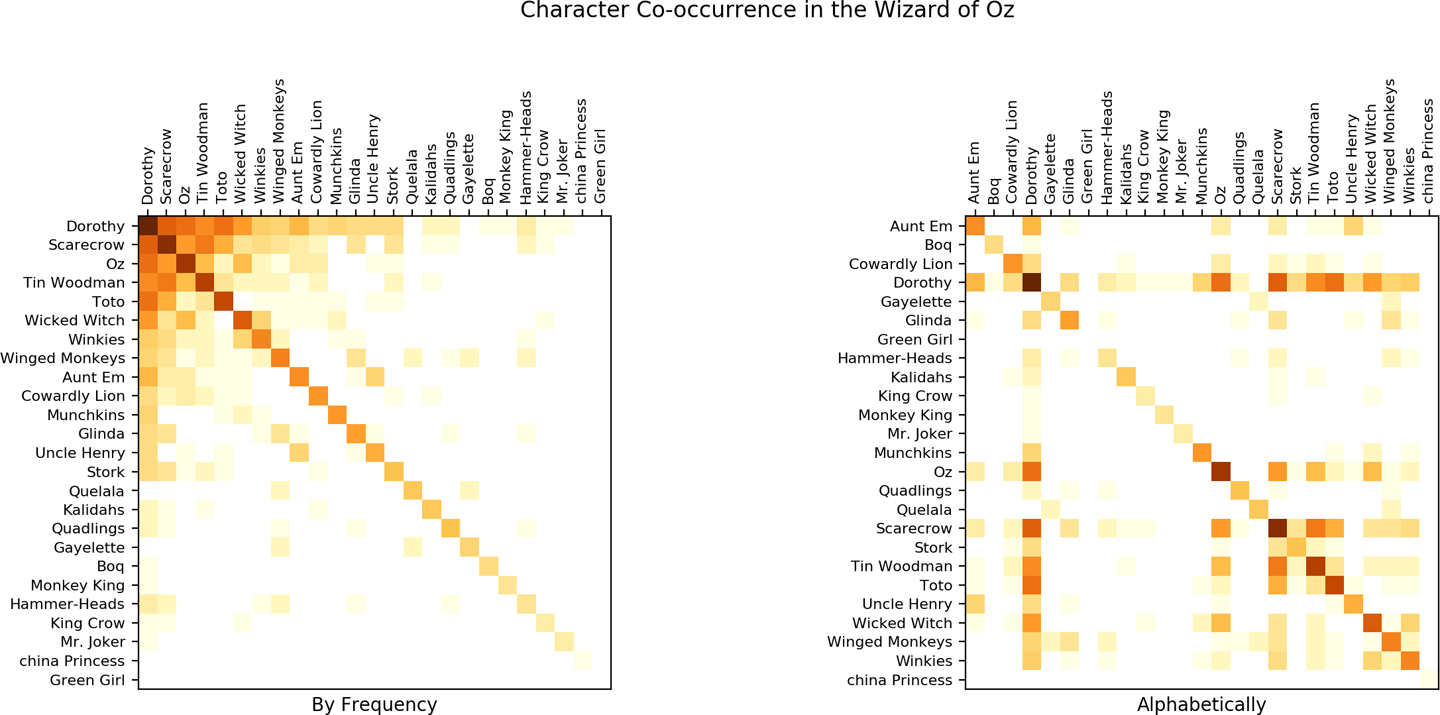
\includegraphics[width=0.8\textwidth]{figures/MatrizCoOcurrencias.png}
        \caption{\label{fig:MatrizCoOcurrencias} Matriz de Co-Ocurrencias del libro Mago de Oz} Fuente: Applied text analysis with python \cite{bengfort2018applied}
    \end{figure}
    \item Gráfico de dispersión: mientras la matriz de co-ocurrencias da una vista general de las relaciones que pueden existir entre personajes, ésta no toma en cuenta cómo una entidad interactúa a lo largo de la narrativa. Los gráficos de dispersión muestran como cierta entidad es nombrada a lo largo del tiempo y, en general, permiten ver en que momentos de un texto cierta entidad es más o menos relevante (ver figrua \ref{fig:DispersionPLot}).
    \begin{figure}[H]
        \centering
        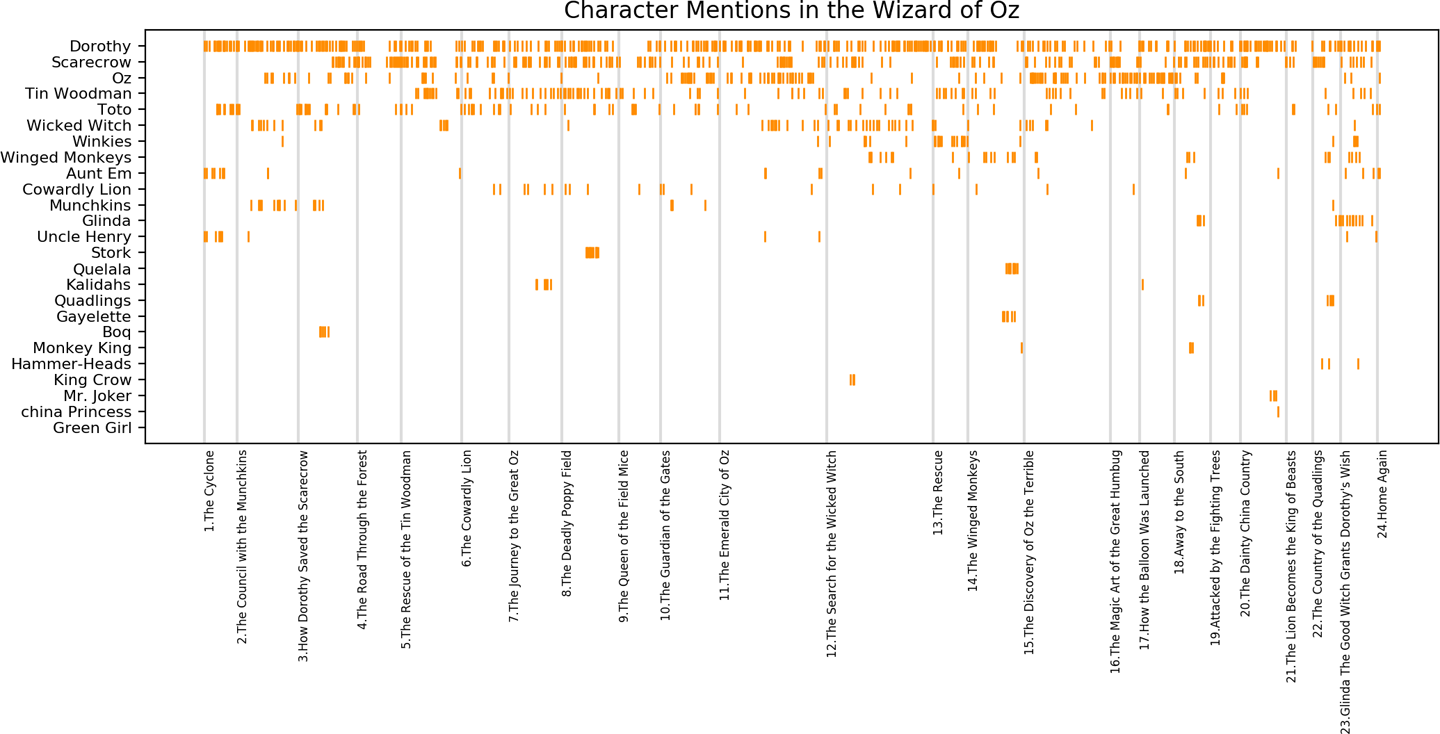
\includegraphics[width=0.8\textwidth]{figures/DispersionPlot.png}
        \caption{\label{fig:DispersionPLot} Gráfico de Dispersión del libro Mago de Oz} Fuente: Applied text analysis with python \cite{bengfort2018applied}
    \end{figure}
\end{enumerate}

\paragraph{Visualización de temas de un corpus de documentos}
\paragraph*{}
    Como se discutió en secciones anteriores, una de las tareas más comunes a la hora de analizar textos es descubrir los temas latentes que habla un corpus en particular. Sin embargo, comunicar este resultado no es para nada trivial por lo que en la literatura se han desarrollado algunas herramientas que permiten visualizar de mejor forma los resultados de dichos algoritmos.
\subparagraph{LDAvis}
\subparagraph*{}
    LDAvis \cite{sievert2014ldavis} es un sistema web utilizado para visualizar los resultados del algoritmo LDA. LDAVis  busca responder tres preguntas: 
    \begin{enumerate}
        \item ¿Cuál es el significado de cada tema encontrado?
        \item ¿Qué tan frecuente es cada tema dentro del corpus de documentos?
        \item ¿Qué relación y qué cosas en común existen entre cada tema encontrado?
    \end{enumerate}
    Para resolver esas tres interrogantes LDAVis (ver figura \ref{fig:LDAVis} ) se compone de dos paneles. El panel izquierdo da una vista global de cómo se distribuyen los temas, lo que nos ayuda a responder las preguntas 2 y 3. En esta vista se plotean los temas como círculos en donde el radio de cada círculo está relacionado al porcentaje de \textit{tokens} del \textit{corpus} que pertenecen al tema encontrado (pregunta 2). Además la posición de cada tema es calculada según la distancia entre temas y luego cada tema es proyectado utilizando PCA a dos dimensiones (pregunta 3). 
    
    Por otro lado, el panel derecho de la visualización entrega un diagrama de barras horizontal que representan a los 30 términos más relevantes para el tema seleccionado en el panel izquierdo (pregunta 1).
    \begin{figure}[H]
        \centering
        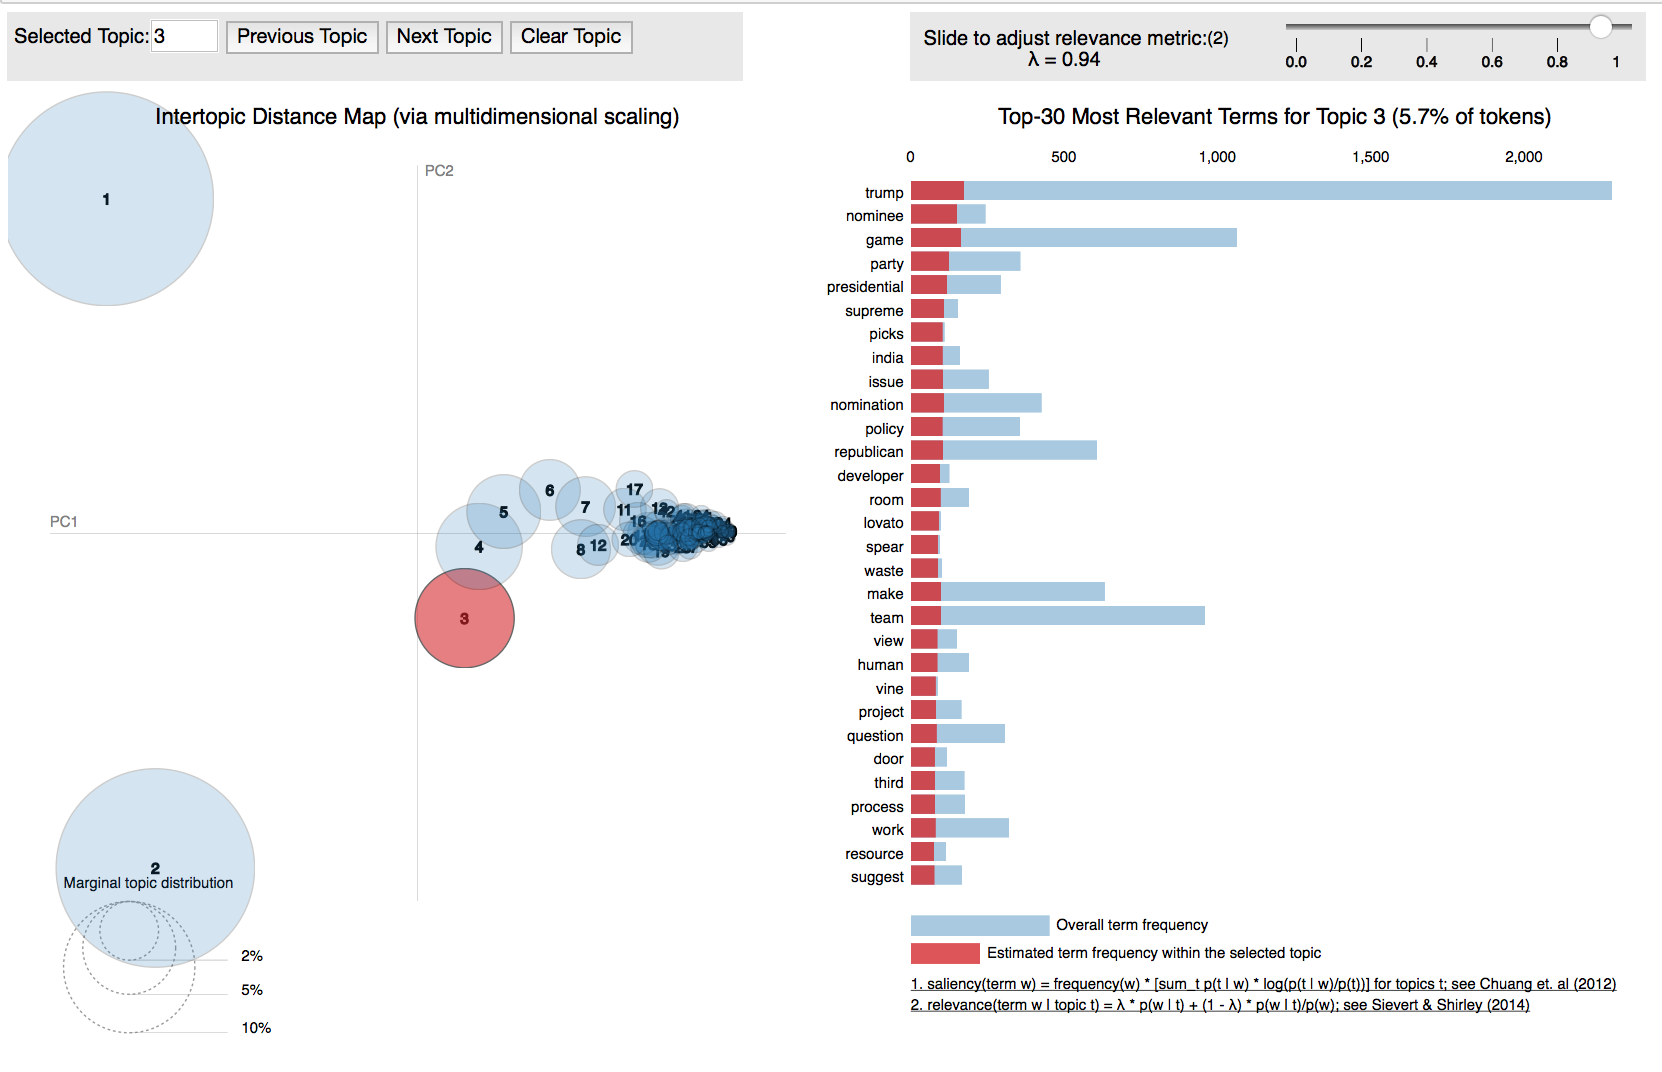
\includegraphics[width=0.8\textwidth]{figures/LDAVis.png}
        \caption{\label{fig:LDAVis} LDAVis} Fuente: LDAvis: A method for visualizing and interpreting topics \cite{sievert2014ldavis}
    \end{figure}
\subparagraph{Visualización para LDA}
\subparagraph*{}
    Otra forma de visualizar los temas extraídos de cierto \textit{corpus} de documentos fue planteado en \cite{kucher2018analysis}. Esta visualización es utilizada para demostrar los resultados de extracción de temas utilizando el algoritmo LDA, y se basa en la visualización LDAVis descrita anteriormente. 
    
   Se compone de tres paneles, denotados por a), b) y c) en la figura 14 que sirve de ejemplo. A continuación se describen los tres paneles por separado:
    
    \begin{itemize}
        \item Panel a) : es un \textit{scatterplot} en donde cada punto es uno de los documentos analizados. Cada uno estos posee N-\textit{Features} que corresponden a la probabilidad de cada documento de pertenecer a uno de los N tópicos encontrados por LDA. El espacio de N temas es reducido a dos utilizando t-SNE y sobre ese nuevo espacio reducido son proyectados los documentos permitiendo visualizar \textit{clusters} de documentos, en este caso los 7 temas más relevantes dentro del \textit{corpus} analizado. Otra cosa que se puede ver en este panel son los colores de cada punto. En este caso el color opaco implica que existe una alta probabilidad del documento de pertenecer al tema asignado mientras que un color transparente nos dice lo contrario.
        
        \item Panel b): es un \textit{barchart} que muestra el porcentaje de términos pertenecientes a cada uno de los tópiocs encontrados por nuestro algoritmo.
        
        \item Panel c): muestra los términos más relevantes para el tema seleccionado en el panel b. Además, entre paréntesis índica la cantidad de veces que aparece el término en dicho tema. Finalmente el color de la barra muestra a qué tema está más relacionado el término en cuestión.
    \end{itemize}
    
    \begin{figure}[H]
        \centering
        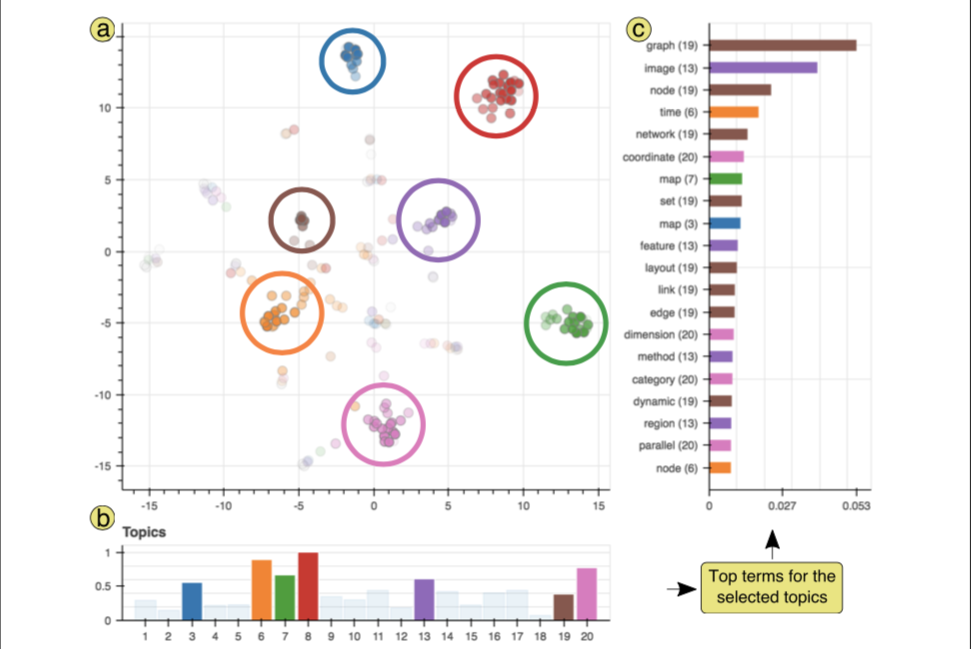
\includegraphics[width=0.8\textwidth]{figures/AnalisisVinci.png}
        \caption{\label{fig:Vinci} Visualización para LDA} Fuente: Analysis of VINCI 2009–2017 Proceedings \cite{kucher2018analysis}
    \end{figure}
    
\paragraph{Visualización de clusters de documentos}
\subparagraph{Visualización para Clustering jerarquico aglomerativo}
\subparagraph*{}
    El proceso de clustering jerárquico aglomerativo puede ser resumido en un \textit{Dendrograma} \cite{everitt1998cambridge}. Este árbol ilustra la serie de pasos que toma el método para formar desde n clusters un único gran cluster que contiene todos los datos analizados (Ver figura \ref{fig:Dendrogram}). 

    \begin{figure}[H]
        \centering
        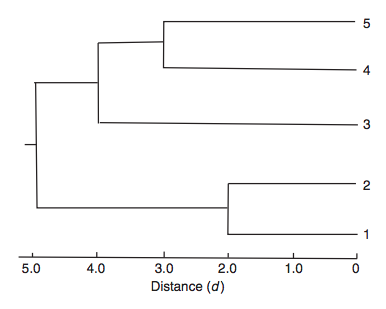
\includegraphics[width=0.8\textwidth]{figures/Dendrogram.png}
        \caption{\label{fig:Dendrogram} Dendrograma} Fuente: 
        The cambridge dictionary of statistics cambridge university press \cite{everitt1998cambridge}
    \end{figure}
    



\newpage
\secnumbersection{PROPUESTA DE SOLUCIÓN}

En el presente capítulo, se explicará la solución propuesta para enfrentar el problema presentado en los capítulos anteriores. Esta se basa, en someter los documentos de la compañía a un proceso de minería y análisis de textos. Para ello, es necesario seleccionar alguna de las metodologías presentadas en el capítulo anterior y definir los experimentos que permitirán extraer la información oculta en dichos activos de la compañía.

\subsection{Metodología}
    La metodología seleccionada para desarrollar este trabajo fue una mezcla entre la propuesta por Kumar (Ver sección 2.2.4) y la propuesta por Google (Ver sección 2.2.5) . Estas metodologías fueron seleccionadas ya que, en primer lugar la propuesta por Kumar entrega la libertad de aplicar cualquier técnica de minería de textos. Por otro lado, la guía desarrollada por Google entrega algunos tips interesantes sobre cómo desarrollar ciertas tareas. Además, según la tabla comparativa (Ver tabla: \ref{table:comparación_metodologías_tm}) estudiada en el
    capítulo anterior, ambas metodología son las que cubren una mayor cantidad de etapas dentro del proceso de minería de textos. 
    
    A continuación, (Ver tabla: \ref{table:My_Methodology})  se puede ver un pequeño resumen de las etapas que serán efectuadas en nuestro proceso de minería de textos. Como se explicó más arriba es una mezcla entre la versatilidad de la metodología propuesta por Kumar y algunos de los tips técnicos propuestos por Google.
    
    \begin{table}[h!]
    \centering
    \begin{tabular}{|c|c|c|}
\hline
\textbf{Etapa}                 & \textbf{Metodología} & \textbf{Descripción}                                                                                                                                                                                                     \\ \hline
Obtención de Datos     & Google                & \begin{tabular}[c]{@{}c@{}}Obtener un conjunto de documentos a \\ analizar. Este conjunto debe ser numeroso ya que \\ se debe poder generalizar los resultados encontrados.\end{tabular}                                                       \\ \hline
Preprocesamiento de Textos     & Kumar                & \begin{tabular}[c]{@{}c@{}}Someter los textos a un proceso de \\ preprocesamiento con el fin de eliminar \\ incongruencias y estandarizar los textos.\end{tabular}                                                       \\ \hline
Análisis Exploratorio de Datos & Google               & \begin{tabular}[c]{@{}c@{}}Encontrar métricas que describan \\ el conjunto de datos a estudiar \\ de forma global como por ejemplo:\\  Número de Textos a estudiar, \\ Promedio de palabras por texto, etc.\end{tabular} \\ \hline
Transformación de Textos       & Google               & \begin{tabular}[c]{@{}c@{}}Encontrar una representación numérica \\ para los datos considerando la \\ técnica de minería de textos \\ que se utilizará en la etapa posterior.\end{tabular}                               \\ \hline
Técnicas de Minería de textos  & Kumar                & \begin{tabular}[c]{@{}c@{}}Ejecutar las técnicas de minería de textos \\ seleccionadas anteriormente.\end{tabular}                                                                                                       \\ \hline
Evaluación                     & Kumar                & \begin{tabular}[c]{@{}c@{}}Evaluar el resultado de las técnicas \\ de minería de textos utilizando\\ la opinión de expertos\\  o métricas de desempeño.\end{tabular}                                                     \\ \hline
\end{tabular}
\caption{\label{table:My_Methodology} Descripción de metodología a utilizar} Fuente: Elaboración Propia
    \end{table}

Una vez seleccionada la metodología para trabajar en el proyecto, se debe describir cómo se desarrollará cada una de las etapas del proceso de minería de textos. 

\subsection{Proceso de minería de textos}

    En la presente sección se describirán cada una de las etapas del proceso de minería de textos, al cual los documentos fueron sometidos utilizando la metodología seleccionada.
    
\subsubsection{Obtención de datos}
    Antes de iniciar un proyecto de minería y análisis de textos, se deben tener los documentos que serán utilizados a lo largo del trabajo. En el caso de esta memoria, los documentos a analizar son las propuestas técnicas de trabajo de la compañía Hatch. Estos archivos se encuentran almacenados en el sistema de gestión documental de la compañía. Sin embargo, el autor de esta memoria no posee los privilegios para ingresar a dicho sistema, por lo que será tarea del personal de Hatch recolectar los documentos a analizar y entregarlos para la ejecución del proyecto.
    
\subsubsection{Preprocesamiento de Textos}
    Tal como se describió en la sección 2.3, existe una gran cantidad de tareas de preprocesamiento que se deben realizar antes de utilizar cualquier técnica de minería de textos. Considerando la cantidad de documentos que se deben analizar se propone construir un \textit{Normalizador de textos}. Esto con el fin de poder estandarizar de forma rápida y eficiente un número considerable de documentos (Ver figura: \ref{fig:normalizador}). 
    
    \begin{figure}[H]
    \centering
    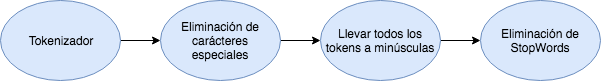
\includegraphics[width=0.8\textwidth]{figures/Normalizador_Textos.png}
    \caption{\label{fig:normalizador} Flujo de preprocesamiento de texto} Fuente: Elaboración Propia.
    \end{figure}
    
    Otra tarea que se debe realizar en esta etapa es el almacenamiento de los documentos en alguna estructura más conveniente para ejecutar las tareas de análisis de forma más rápida y simple. Para ello se propone construir un \textit{json} para cada uno de los documentos a analizar. La estructura de este \textit{json} debe al menos almacenar la siguiente información:
    
    \begin{lstlisting}
    {
        "id": id de la propuesta,
        "proyecto": nombre del proyecto,
        "cliente": cliente de la propuesta,
        "tokens": documento completo tokenizado,
        "keywords_freq": keywords según frecuencia,
        "keywords_pmi": keywords según pmi,
        "estado": estado final de la propuesta ganadora o perdedora,
        "tokens_bigram": bigramas asociados al documento
    }
    \end{lstlisting}
    

\subsubsection{Análisis exploratorio de datos}
    Una vez preprocesados los textos, es importante tener una visión general de los datos que se trabajarán. Esto con el fin de tener en cuenta posibles limitaciones en cuanto a conjunto de técnicas a utilizar e información a extraer. Es por esto que antes de realizar cualquier análisis se deben calcular las siguientes métricas:
    
    \begin{itemize}
        \item \textbf{Número de documentos en la muestra}: Número total de documentos a estudiar.
        \item \textbf{Número de clases}: Número de clases definidas a priori dentro del conjunto de documentos a estudiar.
        \item \textbf{Número de muestras por clase}: Número de muestras pertenecientes a cada clase.
        \item \textbf{Número de palabras por documento}: Mediana de palabras por documento.
    \end{itemize}
    
 
\subsubsection{Transformación de textos}
    Una vez preprocesados todos los textos, éstos deben representarse de manera numérica para poder ser utilizados dentro de cualquier algoritmo de minería de textos (Ver sección 2.4). Tal como se describió en la respectiva sección, se deben realizar dos pasos para lograr este objetivo: Tokenización y Vectorización. En nuestro caso el proceso de Tokenización será efectuado utilizando bolsas de palabras. Por otro lado, dependiendo del algoritmo que se utilizará, las bolsas de palabras serán ponderadas utilizando alguna métrica en particular que será definida al momento de realizar la minería. 
    
    Considerando lo anterior, podemos definir la matriz de documentos $D$ como: La matriz cuyas columnas representan a cada una de las bolsas de palabras encontradas en el corpus, mientras que sus filas representan a cada uno de los documentos pertenecientes al corpus. Considerando esto, el elemento de la matriz $D_{ij}$ será la ponderación de la $j$-ésima bolsa de palabra en el $i$-ésimo documento utilizando alguna métrica en particular.
    
    A modo de ejemplo (Ver tabla: \ref{table:matriz de datos}) se puede ver cómo lucirá la matriz de documentos.
    
    \begin{table}[H]
    \centering
    \begin{tabular}{c|c|c|l|l|}
    \cline{2-5}
    \textbf{}                                       & \textbf{Bolsa $1$} & \textbf{Bolsa $2$} & \textbf{...............} & \textbf{Bolsa $m$} \\ \hline
    \multicolumn{1}{|c|}{\textbf{Documento $1$}}    &                  &                  &                          &                  \\ \hline
    \multicolumn{1}{|c|}{\textbf{Documento $2$}}    &                  &                  &                          &                  \\ \hline
    \multicolumn{1}{|c|}{\textbf{................}} &                  &                  &                          &                  \\ \hline
    \multicolumn{1}{|c|}{\textbf{Documento $n$}}    &                  &                  &                          &                  \\ \hline
    \end{tabular}
     \caption{\label{table:matriz de datos} Representación de corpus} Fuente: Elaboración Propia.
    \end{table}
    
    
\subsubsection{Proceso de minería y análisis de textos}
    Una vez realizados todos los pasos anteriores, llega la parte más vital dentro de un proyecto de minería de textos, la cual es seleccionar las técnicas y/o modelos que entreguen la información que se busca. En el caso de esta memoria, el objetivo del proyecto es encontrar los patrones que ayuden a mejorar el proceso de producción de propuestas técnicas. En seguida se describen los experimentos propuestas para lograr dicho objetivo:

    \paragraph{Análisis mediante el uso de keywords}
    \paragraph*{}
    Como primera aproximación, se deben poder encontrar los elementos que diferencian a una propuesta ganadora de una perdedora, una perdedora de una ganadora y las cosas que estás poseen en común. Para realizar esto, se propone realizar un análisis mediante el uso de \textit{keywords} (Ver sección 2.5.1). El uso de esta técnica, se debe a que debemos realizar un proceso de ''reducción de dimensionalidad´´ para poder, en primer lugar caracterizar cada documento y en segundo lugar poder responder las preguntas planteadas anteriormente, utilizando como elemento a analizar los \textit{keywords} encontrados para cada documento.  
     
    Tal como se comentó en la sección anterior, se debe seleccionar alguna medida numérica para caracterizar a cada una de las bolsas de palabras dentro del corpus. Para el caso de análisis mediante \textit{keywords} se utilizan como medidas: Frecuencia Absoluta y PMI (Ver sección 2.5.1.1).
    
    Una vez realizado el proceso anterior, se espera también poder analizar como los \textit{keywords} , más relevantes en todo el conjunto de documentos, interactúan dentro de las propuestas ganadoras y perdedoras. Para ello, se propone utilizar un gráfico de dispersión léxica (Ver sección 2.5.4.1.1), el cual nos permite visualizar cómo es que ciertos \textit{keywords} se comportan dentro de documentos ganadores y perdedores. El análisis de esto debe ser capaz de responder preguntas tales como: ¿Existen relaciones entre el uso de \textit{keywords} y el resultado de la propuesta?, ¿Es relevante la posición donde se trata cierto \textit{keyword} dentro de una propuesta?
     
    \paragraph{Modelamiento de Tópicos}
    \paragraph*{}
    Considerando que el experimento anterior caracteriza sólo un documento, es necesario utilizar un algoritmo que pueda realizar un análisis a todo el corpus de manera simultánea. Para ello se utilizará algún algoritmo de modelamiento de tópicos (Ver sección 2.5.2).
    
    Para llevar a cabo un análisis de modelamiento de tópicos, en primer lugar se debe seleccionar algún algoritmo apropiado para realizar esta tarea. En nuestro caso se tienen las opciones de los algoritmos: Latent Dirichlent Allocation (Ver sección 2.5.2.1) y Factorización en matriz no negativa (Ver sección 2.5.2.2). Si bien ambos algoritmos realizan el trabajo de encontrar los temas latentes que se tratan dentro del corpus de documentos, en el caso de esta memoria se utilizará LDA. Esto, ya que además de entregar los temas tratados por el corpus, el algoritmo entrega una distribución de probabilidades de pertenencia a algún tema en particular para cada uno de los documentos analizados.
    
    Para generar el modelo utilizando LDA, se deben seleccionar tres parámetros en general: $\alpha$ , $\beta$ y $k$. Además para medir la cálidad de un modelo LDA se utiliza el índice de coherencia, por lo que se puede utilizar esta métrica para modelos con distintos $k$ y seleccionar el modelo con el índice más alto. Sólo variamos $k$ ya que en general los valores $\alpha$ y $\beta$ se dejan constantes. 
    
    Luego de tener el modelo seleccionado, éste se debe comenzar a explorar. En un principio se deben mostrar los tópicos encontrados por el algoritmo y la definición de éstos realizada por el analista. Por otro lado utilizando la composición de temas dentro de cada uno de los documentos es posible responder preguntas como ¿De qué temas se habla en propuestas ganadoras y perdedoras? ¿Existen diferencias en la importancia que se le dedica a ciertos temas entre propuestas ganadoras y perdedoras? ¿Qué tema predomina en el corpus estudiado?
    
    \paragraph{Clustering usando el resultado de modelamiento de tópicos}
    \paragraph*{}
    Una vez terminado el proceso de modelamiento de tópicos es posible utilizar la distribución de probabilidades de cada documento, encontrada por LDA, como \textit{features} de cada documento (Ver tabla:\ref{table:lda_cluster_matrix}). Con esto buscamos encontrar clusters de documentos pero considerando como elementos a agrupar los temas que cada uno de los documentos trata.
    
    \begin{table}[H]
    \centering
    \begin{tabular}{c|c|c|c|c|}
    \cline{2-5}
    \textbf{}                                       & \textbf{\begin{tabular}[c]{@{}c@{}}Probabilidad \\ Tópico 0\end{tabular}} & \textbf{\begin{tabular}[c]{@{}c@{}}Probabilidad\\ Tópico 1\end{tabular}} & \textbf{...............} & \textbf{\begin{tabular}[c]{@{}c@{}}Probabilidad\\ Tópico m\end{tabular}} \\ \hline
    \multicolumn{1}{|c|}{\textbf{Documento $1$}}    &                                                                           &                                                                          &                          &                                                                          \\ \hline
    \multicolumn{1}{|c|}{\textbf{Documento $2$}}    &                                                                           &                                                                          &                          &                                                                          \\ \hline
    \multicolumn{1}{|c|}{\textbf{................}} &                                                                           &                                                                          &                          &                                                                          \\ \hline
    \multicolumn{1}{|c|}{\textbf{Documento $n$}}    &                                                                           &                                                                          &                          &                                                                          \\ \hline
    \end{tabular}
    \caption{\label{table:lda_cluster_matrix} Representación de corpus} Fuente: Elaboración Propia.
    \end{table}
     
     Al ser \textit{clustering} una familia de algoritmos no supervisados (Ver sección 2.5.3) es necesario realizar el proceso de \textit{clustering} con distintos algoritmos y diversas métricas de distancias para encontrar una configuración óptima. En el caso de esta memoria se crearán modelos de \textit{clustering} aglomerativo y de \textit{clustering} basado en centroide, utilizando K-Means. Como los datos están dentro del rango $[0,1]$ se deberán probar las distancias: Jensen-Shannon, Euclideana y de Manhattan para cada modelo. Por otro lado, los algoritmos de \textit{clustering} aglomerativo también deben ser variados con todos los criterios de enlace.
     
     Cuando todos los modelos hayan sido creados se deben comparar utilizando el índice de Silhouette, con el fin de encontrar el modelo óptimo de \textit{clustering}.
     
     Una vez finalizado el proceso de selección de modelo, se debe describir cada uno de los clusters utilizando la \textit{metadata} de cada documento. Esto es, nombre del proyecto, nombre del cliente y tópico dominante en documento, con el fin de encontrar cuáles son los documentos que se parecen y relaciones entre éstos.
     
     Finalmente para poder comunicar los resultados de forma efectiva, se propone desarrollar una  visualización con los resultados encontrados. La idea es reducir la dimensionalidad de los datos a 2 y luego generar un \textit{scatterplot}. Junto a esto, cada dato debe ser coloreado según el clúster que le corresponda y también debe ser dibujado con alguna forma en particular, dependiendo si el documento es ganador o perdedor.
   
\subsubsection{Evaluación de resultados}
    Una vez terminados todos los experimentos del proceso de minería, se deben comunicar los resultados al principal \textit{stakeholder} del proyecto, en el caso de esta memoria la jefa del equipo de desarrollo de propuestas de la compañía. De esta reunión se espera obtener feedback sobre los estudios realizados, validar las conclusiones extraídas y en conjunto definir los hallazgos útiles que serán incluidos en la guía que se espera obtener como producto final de este proyecto.
     
\subsection{Diseño de Guía}
     Al momento de haber finalizado todo el proceso de minería de textos y con la solución ya validada por el principal \textit{stakeholder} del proyecto, se debe producir una guía que resuma los principales hallazgos que ayuden a mejorar el proceso de producción de propuestas técnicas. La idea es que esta guía sea un punteo de ideas y pequeños tips, que fueron posibles gracias al proceso de minería de textos, dado que de alguna forma hacían a una propuesta tener más chances de ganar.

    
\newpage
\secnumbersection{VALIDACIÓN DE LA SOLUCIÓN}

    En el presente capítulo, se describe la implementación de la solución propuesta (Ver capítulo 3) a la problemática planteada en esta memoria. Se comienza describiendo la implementación y los resultados encontrados para cada etapa del proceso de minería de textos. Una vez finalizado esto se muestra la opinión del experto en el dominio de nuestra problemática , la jefa del equipo de desarrollo de propuestas de la compañía. Finalmente se muestra la guía de buenas prácticas para la generación de propuestas técnicas, que es un punteo con todos los hallazgos encontrados y validados por el stakeholder del proyecto.
    
\subsection{Herramientas utilizadas}
    Para el desarrollo de esta memoria se utilizó como herramienta de análisis de datos al lenguaje de programación Python y muchas de sus librerías 
\subsubsection{Python}    
Python Software Foundation (PSF) es una corporación sin fines de lucro que
tiene los derechos de propiedad intelectual detrás del lenguaje de programación Python. Para este proyecto se utilizó la versión de Python 3.6, incluyendo las siguientes librerías:
    \begin{itemize}
        \item \textbf{NLTK \footnote{https://www.nltk.org/}}: Natural Language Tool Kit es una librería del lenguaje Python que nos proporciona distintas funcionalidades para el procesamiento de lenguaje tales como tokenización, lematización, entre otras funcionalidades.
        \item \textbf{Gensim \footnote{https://radimrehurek.com/gensim/}}: Gensim es una librería de python para realizar tareas como modelamiento de temas, indexamiento de documentos y recuperación de la información en grandes conjuntos de documentos. 
        \item \textbf{Scikit-Learn \footnote{https://scikit-learn.org}}: Librería de python para realizar tareas de Machine Learning.
        \item \textbf{Pandas \footnote{https://pandas.pydata.org/}}: Librería utilizada para realizar análisis cuantitativo a datos estructurados en python.
        \item \textbf{PyPDF2 \footnote{http://mstamy2.github.io/PyPDF2/}}: Herramienta utilizada para la manipulación de archivos PDF utilizando Python.
    \end{itemize}
            
\subsection{Proceso de minería de textos}
    En la presente sección se describirán cada una de las etapas del proceso de minería de textos, al cual los documentos fueron sometidos utilizando la metodología seleccionada (Ver sección 3.1).

\subsubsection{Preprocesamiento de Textos}
    Para desarrollar el preprocesador propuesto (Ver sección 3.2.1) se utilizarón algunas funciones propias de Python y sus librerías definidas anteriormente. El normalizador desarrollado, toma como parámetros un conjunto de documentos a normalizar y entrega como salida el mismo conjunto preprocesado.  

    \begin{lstlisting}[language=Python]
    import nltk
    import re
    import string
    from nltk.tokenize.toktok import ToktokTokenizer
    
    #Remove special characters
    def remove_characters_after_tokenization(tokens):
        pattern = re.compile('[{}]'.format(re.escape(string.punctuation)))
        filtered_tokens = filter(None, [pattern.sub('', token) for token in tokens])
        return list(filtered_tokens)
    
    #Remove stopwords
    def remove_stopwords(tokens):
        stopword_list = nltk.corpus.stopwords.words('spanish')
        filtered_tokens = [token for token in tokens if token not in stopword_list]
        return filtered_tokens
    
    def normalizador(corpus):
        normalized_corpus = []
        toktok = ToktokTokenizer()
        for i in range(len(corpus)):
            sample_words = toktok.tokenize(corpus[i])
            sample_words = remove_characters_after_tokenization(sample_words)
            #Documents to lower
            sample_words = list(map(str.lower,sample_words))
            sample_words = remove_stopwords(sample_words)
            normalized_corpus.append(sample_words)
        return normalized_corpus
    \end{lstlisting}
    
    Por otra parte para generar el \textit{json} propuesto en el capítulo anterior, se aprovecho de la estructura de la cabecera de todos los documentos para extraer datos tales como nombre del cliente, nombre del proyecto e identificación de la propuesta (Ver figura \ref{fig:portada_propuesta}). A continuación se presenta el respectivo script:
    
    \begin{lstlisting}[language=Python]
    #Read file
    pdfFileObj = open(file_name,'rb')     
    pdfReader = PyPDF2.PdfFileReader(pdfFileObj)
    #Read page 1
    pageObj_name = pdfReader.getPage(1)
    text = pageObj_name.extractText()
    #Tokenize text 
    text = text.split("\n")
    client = text[0]
    project = text[1]
    id = [i for i in text if re.search("\d{2}-\d{4}", i)]
    \end{lstlisting}
    
    Utilizando este script para cada uno de los documentos, más el resultado del normalizador se puede construir facilmente el \textit{json} para cada uno de los documentos y así tener una estructura de datos más fácil de manipular para posteriores análisis. Cabe destacar que el campo ''estado`` tuvo que ser insertado de manera manual dentro del \textit{json} de cada documento, ya que no existía forma de extraerlo a partir del documento.
    
    \begin{figure}[h!]
    \centering
    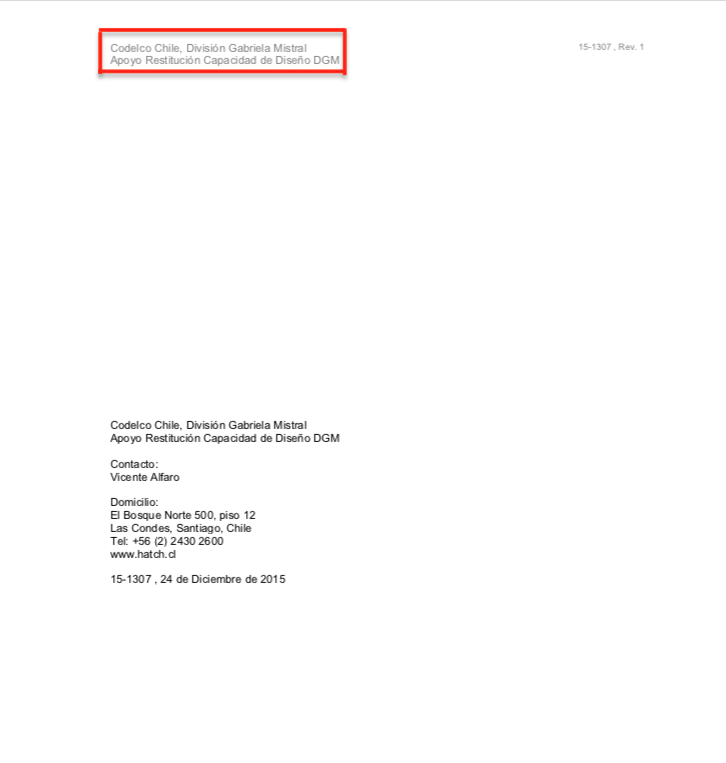
\includegraphics[width=0.8\textwidth]{figures/Header.png}
    \caption{\label{fig:portada_propuesta} Header de una propuesta en general} Fuente: Elaboración Propia.
    \end{figure}
    
    
    
\subsubsection{Análisis exploratorio de datos}
    Una vez preprocesados los textos, es necesario extraer algunas métricas importantes (Ver sección 3.2.2). El corpus a analizar posee un total de 17 documentos en dónde estos han sido clasificados, de manera supervisada, en dos clases: propuestas perdedoras y propuestas ganadoras (Ver tabla: \ref{table:key:_metrics_corpus}).
    
    \begin{table}[H]
    \centering
    \begin{tabular}{|c|c|}
    \hline
    \textbf{Métrica}                                                             & \textbf{Valor} \\ \hline
    \begin{tabular}[c]{@{}c@{}}Número de documentos\\ en la muestra\end{tabular} &   17            \\ \hline
    Número de clases                                                             & 2              \\ \hline
    \end{tabular}
    \caption{\label{table:key:_metrics_corpus} Métricas Corpus}  Fuente: Elaboración Propia 
    \end{table}
    
    Por otro lado, al extraer algunas métricas para cada una de las clases (Ver tabla: \ref{table:key:_metrics}) se puede notar que la mediana de documentos analizados de las propuestas perdedoras es mucho mayor al de las propuestas ganadoras (casi el doble). Además, el número de documentos perdedores a analizar es superior al de los documentos ganadores. 
    
    \begin{table}[H]
    \centering
    \begin{tabular}{|c|c|c|c|}
    \hline
    \textbf{Clase}     & \textbf{Número de propuesta} & \textbf{Mediana de palabras por propuesta} & \textbf{Clientes} \\ \hline
    \textbf{Ganadora}  & 7                            & 111106                                     & 3                 \\ \hline
    \textbf{Perdedora} & 9                            & 213777                                     & 4                 \\ \hline
    \end{tabular}
    \caption{\label{table:key:_metrics} Métricas Claves}  Fuente: Elaboración Propia 
    \end{table}
    
\subsubsection{Transformación de Textos}
    El proceso de transformación de textos depende de cada una de las técnicas que se utilicen (Ver sección 3.2.3). Por ello se describen junto al desarrollo de las técnicas y algoritmos en secciones posteriores . 
    
\subsubsection{Técnicas de Minería de Textos}
    En esta sección se describen en profundidad los experimentos y resultados obtenidos por las técnicas de minería de textos utilizadas en nuetro estudio. 
    
\paragraph{Caracterización de un documento en particular}
\paragraph*{}
    Luego de conocer las métricas claves de nuestro corpus a analizar, también es importante conocer de que habla un documento en general. La forma más sencilla de realizar este ejercicio es utilizando una nube de palabras (Ver sección 2.5.4.1.1). Para realizar esto se seleccionó un documento al azar ganador y otro documento al azar perdedor obteniendo las visualizaciones (Ver figura \ref{fig:nube_ganadora} y \ref{fig:nube_perdedora} ). 
    
    En general, de ambas nubes de palabras se puede ver que conceptos como proyecto, equipo y diseño son los que más destacan en ambos tipos de propuestas. Además esta visualización nos puede ayudar a tener un acercamiento sobre que trata un proyecto en particular. Por ejemplo en la propuesta perdedora (Ver figura \ref{fig:nube_perdedora}) se puede ver que se está vendiendo un proyecto de ingeniería báscia para el cliente Codelco División Teniente en materias de manejo de materiales. 

\begin{figure}[H]
\centering
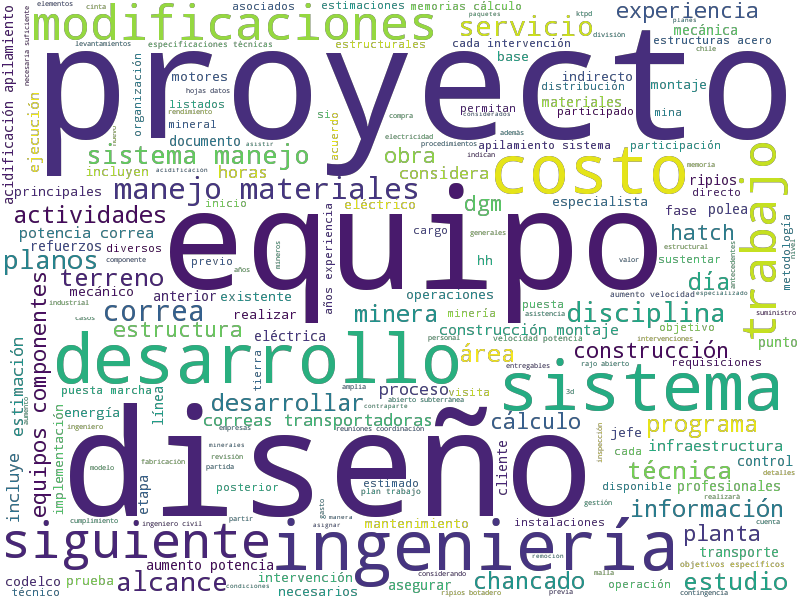
\includegraphics[width=0.8\textwidth]{figures/KeyWords/nube_ganadora.png}
\caption{\label{fig:nube_ganadora} Nube de Palabras de una propuesta ganadora} Fuente: Elaboración Propia.
\end{figure}

\begin{figure}[H]
\centering
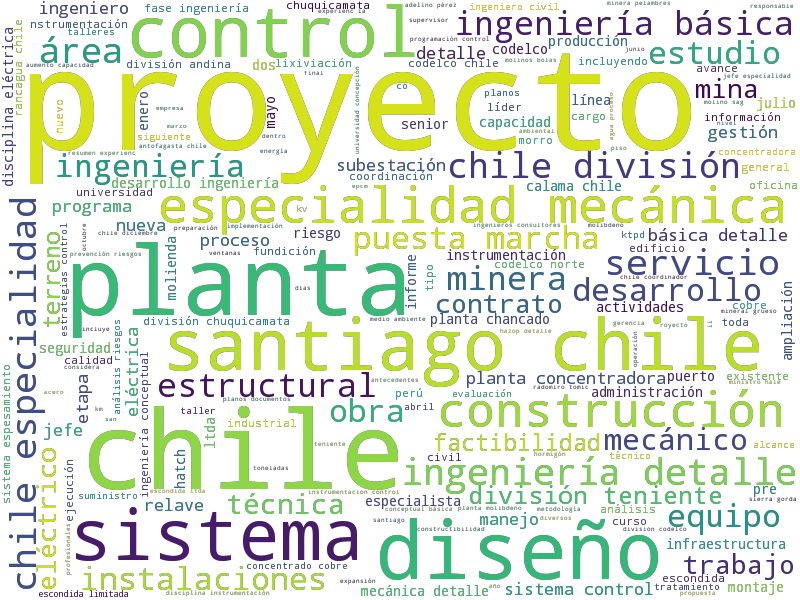
\includegraphics[width=0.8\textwidth]{figures/KeyWords/nube_perdedora.png}
\caption{\label{fig:nube_perdedora} Nube de Palabras de una propuesta perdedora} Fuente: Elaboración Propia.
\end{figure}

\paragraph{Extracción de KeyWords}
\paragraph*{}
    El objetivo principal del estudio que se está desarrollando, es lograr caracterizar y en lo posible encontrar los patrones que permitan diferenciar a una propuesta ganadora de una perdedora. Teniendo esto en cuenta, se definió que el primer paso que se debía dar era poder entender que hablaba cada una de las propuestas analizadas. Como se vio en la sección anterior, una buena forma de realizar esto era utilizando nubes de palabras pero ¿Será útil realizar esto mismo para un corpus de documentos?, ¿Es viable analizar $n$ nubes de palabras con el fin de entender todo el corpus en cuestión? Las respuestas a todas estas interrogantes anteriores son negativas. Sin embargo, para lograr este objetivo se puede utilizar el proceso de extracción de KeyWords (Ver sección sección 2.5.1) el cual hace uso de n-gramas y nos permitirá caracterizar a un corpus completo de documentos.

\subparagraph{Proceso de extracción de n-gramas y rankeo}
\subparagraph*{}
    Tal como se describe en la sección 2.5.1, para extraer un keyword de un documento en particular. lo primero que se debe realizar es romper el documento en n-gramas. En el caso de esta memoria se decidió analizar al corpus utilizando 2-gramas. Para realizar esto, se puede utilizar el siguiente scrtipt:

    \begin{lstlisting}[language=Python]
    import nltk
    finder = BigramCollocationFinder.from_words(text_tokenized, window_size = 3)
    \end{lstlisting}
    
    Cabe destacar que el script anterior, recibe como parametro un texto tokenizado, como por ejemplo, el retornado por nuestro normalizador y retorna el texto en 2-gramas.
    
    Una vez realizado este proceso, los 2-gramas (que desde ahora llamaremos bolsas de palabras) deben ser rankeados utilizando alguna métrica. Esto, con el fin de poder encontrar las bolsas de palabras más relevantes dentro del corpus. Para este paso, se utilizarón dos métricas (Ver sección 2.5.1) :
    
    \begin{itemize}
        \item Frecuencia absoluta
        \item Información mutua puntual
    \end{itemize}
    
    Se puede obtener dicho ranking utilizando el siguiente script:
    \begin{lstlisting}[language=Python]
    from nltk.collocations import *
    bigram_measures = nltk.collocations.BigramAssocMeasures()
    #Bow using absolute frequency 
    bow_freq = []
    for k,v in finder.ngram_fd.items():
        bow_freq.append((k,v))
    #Bow using pmi
    bow_pmi = finder.score_ngrams(bigram_measures.pmi)
    \end{lstlisting}
    
     Una vez rankeados todos los documentos, se debió seleccionar un criterio para detectar a las bolsas de palabras \textit{Top} para cada una de las métricas utilizadas, estas bolsas serán los keywords. Cuando hablamos de keywords nos referimos a las bolsas de palabras más relevantes según la métrica que estemos utilizando dentro de un documento $d$. 
    
    Para realizar este proceso, se decidió seleccionar un umbral para cada una de estas métricas y así las bolsas de palabras que estuvieran sobre este umbral serían \textit{keywords} y en caso contrario serían una bolsa normal. Para seleccionar este umbral, se tomó un documento al azar y se realizó el plot \textit{Número de bolsas de Palabras Vs Frecuencia Absoluta y PMI} respectivamente.
    
    El resultado de este pequeño experimento para la métrica frecuencia absoluta (Ver figura: \ref{fig:BowVsFA} ) fue de 20 apariciones dentro de un documento. Es decir la0s bolsas de palabras que aparecieran más de 20 veces dentro de un documento se consideran como keywords. Esta elección se hizo ya que la idea de encontrar keywords era disminuir el número de bolsas a analizar posteriormente y como se puede apreciar en el gráfico (Ver figura \ref{fig:BowVsFA}) la mayoría de las bolsas se concentran en frecuencias entre 0 y 10. Y pocas bolsas son las que tienen una frecuencia superior a 20 , es decir pocas bolsas son las que aparecen mucho en el documento.
    
    \begin{figure}[H]
    \centering
    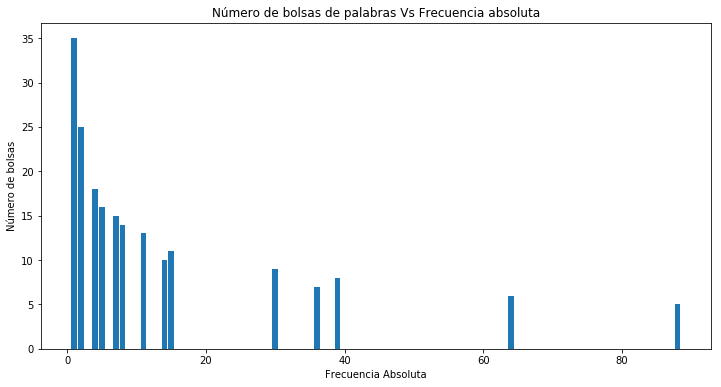
\includegraphics[width=0.8\textwidth]{figures/KeyWords/Umbral_FA.png}
    \caption{\label{fig:BowVsFA} Número de Bolsas Vs Frecuencia Abosluta} Fuente: Elaboración Propia.
    \end{figure}
    
    Por otro lado el resultado para la métrica de información mutua puntual (Ver figura \ref{fig:BowVsPMI} ) fue bastante desalentador. Como se puede apreciar en la figura existían más de 800 bolsas con un PMI superior a 12 por lo que el objetivo de extraer un número bajo de keywords no se cumple usando está métrica. 
    Considerando lo anterior de aquí en adelante se utilizarán los keywords extraídos utilizando la metrica de frecuencia absoluta. 
    
    \begin{figure}[H]
    \centering
    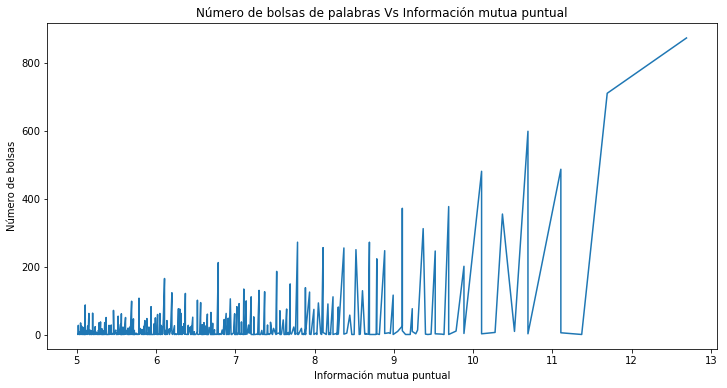
\includegraphics[width=0.8\textwidth]{figures/KeyWords/Umbral_PMI.png}
    \caption{\label{fig:BowVsPMI} Número de Bolsas Vs Información  Mutua Puntual} Fuente: Elaboración Propia.
    \end{figure}

\subparagraph{Comparación de keywords de propuestas ganadoras y perdedoras}
\subparagraph*{}
    Una vez extraídos los \textit{keywords} de todos los documentos tanto ganadores como perdedores, se prosiguió a intentar caracterizar al conjunto de documentos ganadores y al conjunto de documentos perdedores. Para ello se agruparon todos los \textit{keywords}, que al menos aparecieran en dos o más documentos, dentro de las propuestas ganadores y perdedores. Una vez realizado este proceso se obtuvieron los conjuntos $G$ y $P$ que almacenaban los \textit{keywords} para las propuestas ganadores y perdedoras respectivamente. 
    
    Considerando que tenemos dos conjuntos de \textit{keywords}, se optó por realizar operaciones de conjuntos con el fin de encontrar los conceptos comunes entre documentos ganadores y perdedores, además de \textit{keywords} que sólo aparecen en documentos ganadores mas no en perdedores y vice-versa.
    
    A continuación se presentan las operaciones utilizadas y una breve interpretación de sus resultados:
    
    \begin{itemize}
        \item $G \cap P$: La intersección entre los keywords ganadores y perdedores (Ver tabla: \ref{table:Conceptos_comunes}) es interpretada como el conjunto de elementos básicos dentro de cualquier propuesta. 
        
        \begin{table}[H]
        \centering
        \begin{tabular}{|c|c|}
        \hline
        \textbf{Concepto 1} & \textbf{Concepto 2} \\ \hline
        Años                & Experiencia         \\ \hline
        Desarrollo          & Ingeniería          \\ \hline
        Específicaciones    & Técnicas            \\ \hline
        Gestión             & Cálidad             \\ \hline
        Ingeniería          & Básica              \\ \hline
        Ingeniería          & Detalles            \\ \hline
        Lider               & Disciplina          \\ \hline
        Plan                & Cálidad             \\ \hline
        Prevencion          & Riesgos             \\ \hline
        Salud               & Ocupacional         \\ \hline
        Seguirdad           & Salud               \\ \hline
        Sistema             & Gestión             \\ \hline
        \end{tabular}
        \caption{\label{table:Conceptos_comunes} Conceptos comunes en cualquier propuesta} Fuente: Elaboración Propia
        \end{table}
        
        De aquí se puede apreciar que elementos como ``Gestión de Cálidad'', ``Prevención de Riesgos'' , ``Sistemas de Gestión'' son temas que son tratados en la mayoría de las propuestas de la compañía. Por otro lado, adjetivos positivos para calificar a la compañía como \textit{``Años de Experiencia''}, \textit{``Líder Disciplina''} también son utilizados para cualquier propuesta.
        
        \item $G - P$: La diferencia entre los \textit{keywords} ganadores y perdedores puede ser interpretada como los elementos que fueron resaltados en las propuestas ganadoras mas no en las perdedoras (Ver tabla: \ref{table:Conceptos_con_valor}). Esto quiere decir que podrían ser elementos que entregaron valor a la propuesta para hacerla ganadora.
        
        \begin{table}[H]
        \centering
        \begin{tabular}{|c|c|}
        \hline
        \textbf{Concepto 1} & \textbf{Concepto 2} \\ \hline
        Calidad             & Hatch               \\ \hline
        Cliente             & Hatch               \\ \hline
        Control             & Documentos          \\ \hline
        Coordinador         & Calidad             \\ \hline
        Ejecución           & Servicios           \\ \hline
        Estándar            & Cuidado             \\ \hline
        Evaluación          & Todas               \\ \hline
        Medio               & Ambiente            \\ \hline
        Obras               & Anexas              \\ \hline
        Modelo              & Dinámico            \\ \hline
        Ingeniería          & Cierre              \\ \hline
        \end{tabular}
        \caption{\label{table:Conceptos_con_valor} Conceptos que entregan valor a una propuesta} Fuente: Elaboración Propia
        \end{table}
        
        Aquí se puede apreciar como por ejemplo, vincular los conceptos Clientes, Calidad y Hatch tuvo resultados positivos en el resultado de algunas propuestas. Además también se puede ver como hablar sobre prácticas que realiza la compañía sobre ciertos procesos, traen un buen impacto en el resultado final de una propuesta. Como por ejemplo \textit{''Estándar Cuidado``}, \textit{''Evaluación Todas``}, \textit{''Coordinador Calidad``}, \textit{''Control de Documentos``}.
        
        \item $P - G$: La diferencia entre los \textit{keywords} perdedores y ganadores (Ver tabla: \ref{table:Conceptos_sin_valor}) puede ser interpretada como los elementos que fueron resaltados en las propuestas perdedoras mas no en las ganadoras. Esto quiere decir que es probable que estos \textit{keywords} no ayudaron a ganar la propuesta.
        
        \begin{table}[H]
        \centering
        \begin{tabular}{|c|c|}
        \hline
        \textbf{Concepto 1} & \textbf{Concepto 2} \\ \hline
        Civil               & Estructural         \\ \hline
        Compañía            & Minera              \\ \hline
        Disciplina          & Mecánica            \\ \hline
        Diseño              & Planos              \\ \hline
        Ingenieros          & Consultores         \\ \hline
        Ingeniería          & Conceptual          \\ \hline
        Jefe                & Disciplina          \\ \hline
        Manejo              & Materiales          \\ \hline
        Puesta              & Marcha              \\ \hline
        \end{tabular}
        \caption{\label{table:Conceptos_sin_valor} Conceptos importantes en propuestas perdedoras pero no en ganadoras} Fuente: Elaboración Propia
        \end{table}
    \end{itemize}
    Si bien se le podría otorgar una connotación negativa a muchos de estos conceptos, en la práctica esto es imposible de hacer. Esto se debe a que, por ejemplo, los conceptos ``Ingeniería Conceptual'', ``Civil Estructural'' y ''Diseño de Planos`` son disciplinas en sí mismas por lo que claramente estarán siempre en una propuesta de Construcción, por ejemplo. Es por lo anterior que esté conjunto de \textit{keywords} no entrega información utilizable.
\subparagraph{Análisis temporal de keywords comunes para una propuesta} 
\subparagraph*{}
    Del análisis anterior, se extrajo una lista de \textit{keywords} que fueron identificados como elementos básicos dentro de una propuesta. Una pregunta interesante de responder sería ¿Cómo interactúan estos keywords a lo largo de todos los documentos analizados? Para responder a esto podemos hacer uso de un gráfico de dispersión léxica (Ver sección 2.5.4.1.1) .
    
    Antes de explicar los resultados encontrados, es necesario detallar el modo en como se utilizó el gráfico de dispersión léxica. En general, un gráfico de dispersión léxica se utiliza para ver como se comporta una serie de conceptos a lo largo de un documento. En nuestro caso como se desea analizar el comportamiento de \textit{keywords} en un conjunto de documentos, se realizó una pequeña modificación a la visualización original. Esta consiste en analizar un único concepto por gráfico. Para lograr esto, en el eje Y en vez de escribir los conceptos a analizar, se escribieron el nombre de los documentos analizados. Por otro lado, el eje X sigue mostrando la temporalidad del texto en su forma relativa (posición de la palabra dividida en el largo del documento), mientras que en el título del gráfico se puede ver que \textit{keyword} se está analizando. Con esto se pudo comparar como un único concepto era tratado en distintos documentos tanto ganadores como perdedores.
    
    \begin{lstlisting}[language=Python]
    def dispersion_plot_1_token(documents,token,color="blue",y_axis="id"):
        points = []
        for y in range(len(documents)):
            for x in range(len(documents[y]["Tokens_bigram"])):
                if (documents[y]["Tokens_bigram"][x] == token):
                    points.append(((x*100)/len(documents[y]["Tokens_bigram"]),y))
            if points:
                x,y = list(zip(*points))
            else:
                x = y = ()
        yticks = [i["id"] for i in documents]
        if (y_axis != "id"):
            yticks = [i["Proyecto"][0:45] for i in documents]
        fig, ax = plt.subplots(figsize=(12,6))
        plt.plot(x, y, "|", color=color, scalex=.1)
        plt.tick_params(
            axis='x', which='both', bottom='off', labelbottom='off'
        )
        plt.xlabel('Temporalidad del texto')
        plt.yticks(list(range(len(documents))),yticks)
        plt.ylim(-1, (len(documents)))
        plt.title("Análisis de dispersión léxica para " + str(token) + " en propuestas " + documents[0]["Estado"]+"s")
        plt.savefig("img/DispersionPlot_"+str(token)+"_"+color,bbox_inches='tight')
        plt.show()
    \end{lstlisting}
    
    La función anterior recibe como parámetros al conjunto de documentos, en el formato \textit{json} definido en el capítulo anterior y el token a analizar. Además se da la opción de seleccionar el color de las barras del gráfico de dispersión léxica.
    
    A continuación, se describen los hallazgos más importantes que se pudieron recabar realizando este análisis. Cabe destacar que muchos \textit{keywords}, si bien fueron analizados, no se encontró ningún patrón relevante por lo que no se añadió a la discusión.
    
    \begin{itemize}
        \item \textbf{Salud Ocupacional}: Como se puede apreciar en 3 de las propuestas ganadoras (Ver figura: \ref{fig:SO_Win} ) hay una sección completa dedicada a aspectos de salud ocupacional. Sin embargo es difícil dar una connotación positiva a esto ya que en las 4 propuestas restantes el concepto se menciona en puntos específicos del texto e incluso en algunos no se llega a nombrar. Por otro lado en las propuestas perdedoras (Ver figura: \ref{fig:SO_Loss}) se puede apreciar que varios documentos poseen una sección dedicada a temas de salud ocupacional tal como pasaba en algunos documentos ganadores. Sin embargo hay una diferencia sustancial entre estos documentos y los ganadores y es que en los documentos ganadores, se puede ver que el concepto es tratado desde el comienzo en forma paulatina hasta que llega a una sección completamente dedicada a él. Por otro lado, en los documentos perdedores que poseen una sección dedicada a salud ocupacional se puede apreciar como el concepto es tratado a lo largo de todo el texto, con incluso secciones separadas tanto al inicio como el final (posibles anexos). 
        
        \begin{figure}[H]
        \centering
        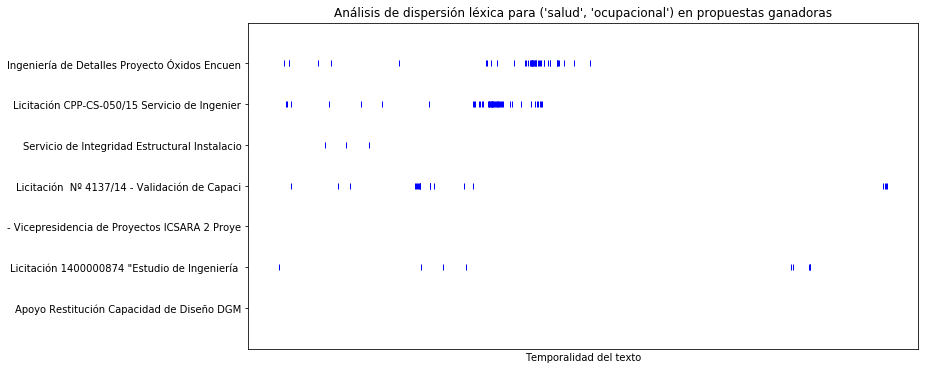
\includegraphics[width=0.8\textwidth]{figures/KeyWords/DispersionPlot_(salud,ocupacional)_blue.png}
        \caption{\label{fig:SO_Win} Dispersión Léxica del concepto Salud Ocupacional en propuestas ganadoras} Fuente: Elaboración Propia.
        \end{figure}
            
        \begin{figure}[H]
        \centering
        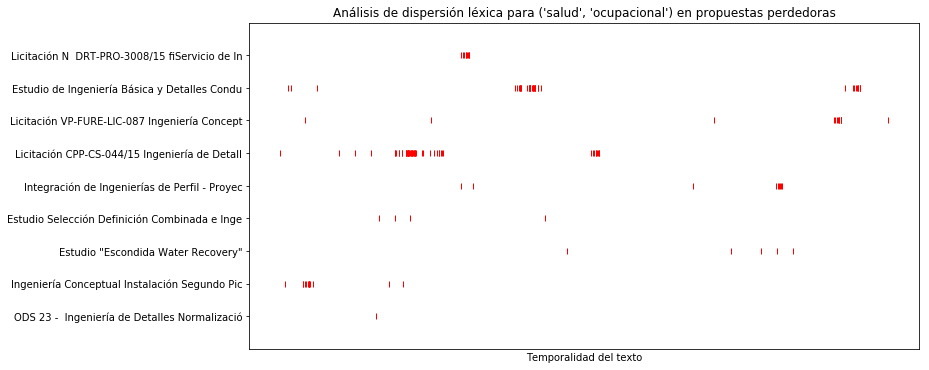
\includegraphics[width=0.8\textwidth]{figures/KeyWords/DispersionPlot_(salud,ocupacional)_red.png}
        \caption{\label{fig:SO_Loss} Dispersión Léxica del concepto Salud Ocupacional en propuestas perdedoras} Fuente: Elaboración Propia.
        \end{figure}
        
        \item \textbf{Gestión de Calidad}: Como se puede apreciar en general, las propuestas perdedoras (Ver figura: \ref{fig:GC_Loss}) poseen un apartado especial sobre Gestión de Calidad. Sin embargo, este concepto no está en un lugar específico para todos los documentos, por ejemplo se puede ver que en el proyecto \textit{Estudio ``Escondida Water Recovery''} la sección del concepto estudiado se encuentra al final del documento, mientras que en el resto de documentos analizados está se encuentra más al inicio. Por otro lado, para los documentos ganadores, (Ver figura: \ref{fig:GC_Win} ) se puede apreciar que si bien ciertos documentos poseen una sección de Gestión de Calidad existen muchos que no la tienen. Además tal como ocurre en las propuestas perdedoras, no existe un lugar específico en dónde tratar este concepto dentro de los documentos por lo que no podemos darle connotaciones negativas ni positivas al lugar donde se utiliza el concepto.
        
        \begin{figure}[H]
        \centering
        \includegraphics[width=0.8\textwidth]{figures/KeyWords/DispersionPlot_(gestión,calidad)_blue.png}
        \caption{\label{fig:GC_Win} Dispersión Léxica del concepto Gestión de Calidad en propuestas ganadoras} Fuente: Elaboración Propia.
        \end{figure}
        
        \begin{figure}[H]
        \centering
        \includegraphics[width=0.8\textwidth]{figures/KeyWords/DispersionPlot_(gestión,calidad)_red.png}
        \caption{\label{fig:GC_Loss} Dispersión Léxica del concepto Gestión de Calidad en propuestas ganadoras} Fuente: Elaboración Propia.
        \end{figure}
    \end{itemize}

    \paragraph{Modelamiento de Tópicos}
    \paragraph*{}
    El siguiente experimento que se debe realizar, es el de modelamiento de tópicos (Ver sección 3.2.4.2). La idea ahora es analizar a los documentos considerando los temas latentes que tratan estos.  
    
    \subparagraph{Transformación de textos}
    \subparagraph*{}
    Como en todo algoritmo de minería de textos, antes de poder ser utilizado es necesario efectuar una transformación a los textos de tal forma que puedan ser interpretados por la técnica a utilizar. En nuestro caso el algoritmo LDA recibe como parámetros un diccionario de palabras de la forma: \textit{(palabra , frecuencia)} con el fin de poder ponderar la importancia de cada palabra dentro de un documento en específico. El resultado para un documento en particular se puede apreciar a continuación:
    
    \begin{lstlisting}[language=Python]
    [[(0, 1), (1, 2), (2, 1), (3, 1), (4, 1), (5, 1), (6, 5), (7, 1), (8, 1), (9, 2), (10, 1), (11, 1), (12, 1), (13, 1), (14, 1), (15, 1), (16, 1), (17, 1), (18, 1), (19, 1), (20, 1), (21, 1), (22, 2), (23, 1), (24, 1), (25, 1), (26, 1), (27, 1), (28, 1), (29, 1), (30, 1), (31, 1), (32, 1), (33, 1), (34, 1), (35, 1), (36, 1), (37, 1), (38, 1), (39, 1), (40, 1), (41, 1), (42, 1), (43, 1), (44, 1), (45, 1), (46, 1), (47, 1), (48, 1), (49, 1), (50, 1)]]
    \end{lstlisting}
    
    \subparagraph{Construcción y parametrización del  modelo}
    \subparagraph*{}
    
    Como se describió en las secciones anteriores, para la construcción de un modelo LDA es necesaria la elección de 3 parámetros: Alfa, Beta y K (número de temas) . Los hiper-parámetros alfa y beta, son relacionados a la variabilidad buscada en los temas y documentos analizados, por lo que en general poseen valores estándares seleccionados. Por otro lado seleccionar el número $k$ adecuado de temas a modelar es una tarea que merece un tratamiento un poco más elaborado. 
    
    Para poder hacer una buena elección del número $k$ de temas a modelar, se puede utilizar el valor de coherencia para un modelo lda con un $k$ en particular. Dentro de esta memoria, se crearon modelos para distintos valores de $k$ (ver figura \ref{fig:Coherence}) y se calculó el número de coherencia para cada uno de ellos. En general se puede apreciar que el índice de coherencia aumenta hasta un $k=8$ y luego de este valor el índice comienza a descender por lo que se utilizará este valor para crear el modelo a analizar.
    
    \begin{figure}[h!]
        \centering
        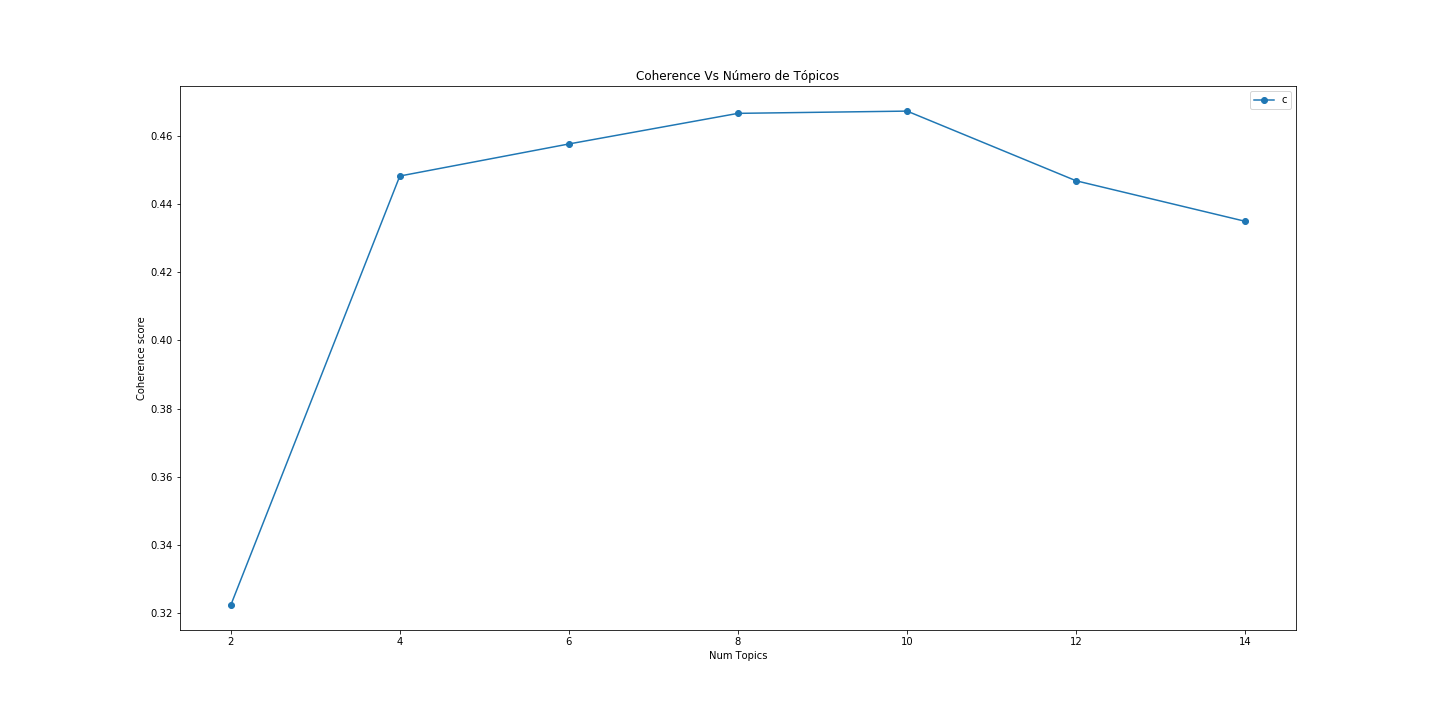
\includegraphics[width=0.8\textwidth]{figures/LDA/Coherence.png}
        \caption{\label{fig:Coherence} Índice de Coherencia Vs Número de Tópicos} Fuente: Elaboración Propia.
    \end{figure}
    
    Una vez creado el modelo, se puede comenzar a ver sus resultados. En este caso se encontraron 8 temas y como se sabe, se puede visualizar cada uno de ellos como una distribución de palabras. A continuación, se puede ver en detalle la composición de cada uno de los temas encontrados: 
    
    \begin{itemize}
        \item \textbf{Tema 0}: 0.011*jefe + 0.010*obras + 0.010*relaves + 0.007*seguridad + 0.007*aguas + 0.007*sistema + 0.007*diseño + 0.007*estudio + 0.007*conducción + 0.006*ambiental
        
        \item \textbf{Tema 1}: 0.013*parte + 0.012*contrato + 0.011*cliente + 0.011*servicios + 0.007*ser + 0.006*información + 0.006*codelco + 0.006*siguientes + 0.006*cualquier + 0.006*acuerdo
        
        \item \textbf{Tema 2}: 0.024*planta + 0.017*cobre + 0.012*prefactibilidad + 0.012*estudio + 0.011*lixiviación + 0.011*análisis + 0.010*control + 0.009*operación + 0.008*caso + 0.007*nacional

        \item \textbf{Tema 3}: 0.015*process + 0.012*fundición + 0.010*smelter + 0.009*copper + 0.009*planta + 0.009*project + 0.008*plant + 0.008*engineer + 0.008*chuquicamata + 0.008*procesos

        \item \textbf{Tema 4}: 0.018*relaves + 0.012*andina + 0.010*obras + 0.009*estudio + 0.008*agua + 0.008*región + 0.007*análisis + 0.006*etapa + 0.006*aguas + 0.006*tranque
        
        \item \textbf{Tema 5}: 0.011*seguridad + 0.011*sistema + 0.011*chancado + 0.010*diseño + 0.010*gestión + 0.009*construcción + 0.008*planos + 0.008*ejecución + 0.007*información + 0.007*control
        
        \item \textbf{Tema 6}: 0.017*planta + 0.011*sistema + 0.011*minera + 0.010*diseño + 0.009*control + 0.008*disciplina + 0.008*detalles + 0.008*equipos + 0.008*codelco + 0.007*manejo
        
        \item \textbf{Tema 7}: 0.023*calidad + 0.011*control + 0.011*codelco + 0.011*desarrollo + 0.010*gestión + 0.009*servicio + 0.008*procesos + 0.007*documentos + 0.007*cumplimiento + 0.007*procedimientos
    \end{itemize}
    
    \subparagraph{Interpretación del modelo}
    \subparagraph*{}
    Una vez obtenido el modelo LDA comienza la parte más compleja de este, la cual es, interpretar los resultados encontrados. Lo primero que se debe realizar cuando se obtienen los temas subyacentes al corpus estudiado, es intentar asignarles algún nombre fácil de identificar (Ver tabla: \ref{table:Topics_Name} ). En nuestro caso, se logró asignarle el nombre a cada uno de los temas con ayuda de expertos en el dominio.
    
    \begin{table}[H]
    \centering
    \begin{tabular}{|c|c|}
    \hline
    \textbf{Tema} & \textbf{Nombre}               \\ \hline
    0             & Seguridad e Impacto Ambiental \\ \hline
    1             & Atención al cliente           \\ \hline
    2             & Cobre                          \\ \hline
    3             & Fundición                     \\ \hline
    4             & Tratamiento de Relaves        \\ \hline
    5             & Construcción        \\ \hline
    6             & Minería                              \\ \hline
    7             & Gestión de Cálidad            \\ \hline
    \end{tabular}
    \caption{\label{table:Topics_Name} Nombres para Tópicos encontrados} Fuente: Elaboración Propia
    \end{table}
    
    Una forma de interpretar los resultados de LDA, es asignar a cada documento su tópico más representativo. Para realizar esto, simplemente se asigna el documento al tópico cuya probabilidad es más alta dentro de su propia distribución de probabilidades. En nuestro caso, se puede apreciar como la mayoría de los documentos analizados (Ver figura: \ref{fig:FreqperTopic}) hablan en su mayoría del tópico Gestión de Calidad. Además, también se puede apreciar como sólo un documento pertenece a los tópicos Fundición y Cobre respectivamente.
    
    \begin{figure}[H]
        \centering
        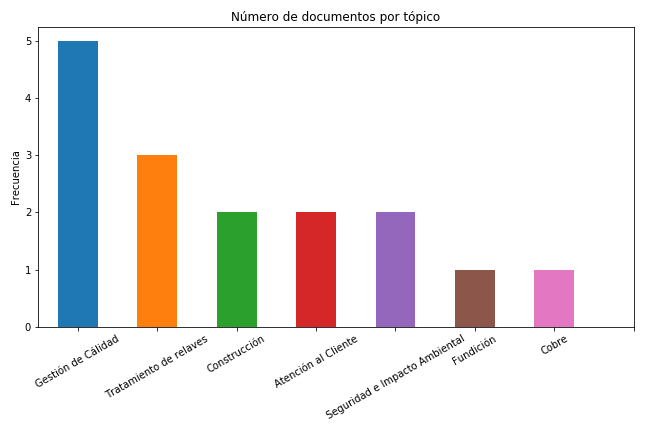
\includegraphics[width=0.8\textwidth]{figures/LDA/documents_per_topic.png}
        \caption{\label{fig:FreqperTopic} Frecuencia de documentos por tópico} Fuente: Elaboración Propia.
    \end{figure}
    
    El mismo análisis efectuado anteriormente, se puede realizar un poco más fino, esta vez viendo cual es la probabilidad de cada documento de pertenecer a cierto tópico. Para realizar esto se creó un gráfico de barras para cada uno de los 8 tópicos (Ver figura: \ref{fig:TopicPerDoc}), en dónde las barras muestran la probabilidad de cada documento de pertenecer al tópico $i$. Para ver una diferencia entre documentos ganadores y perdedores se optó por pintar de azul las propuestas ganadores y de rojo las perdedoras.
    
    \begin{figure}[h!]
        \centering
        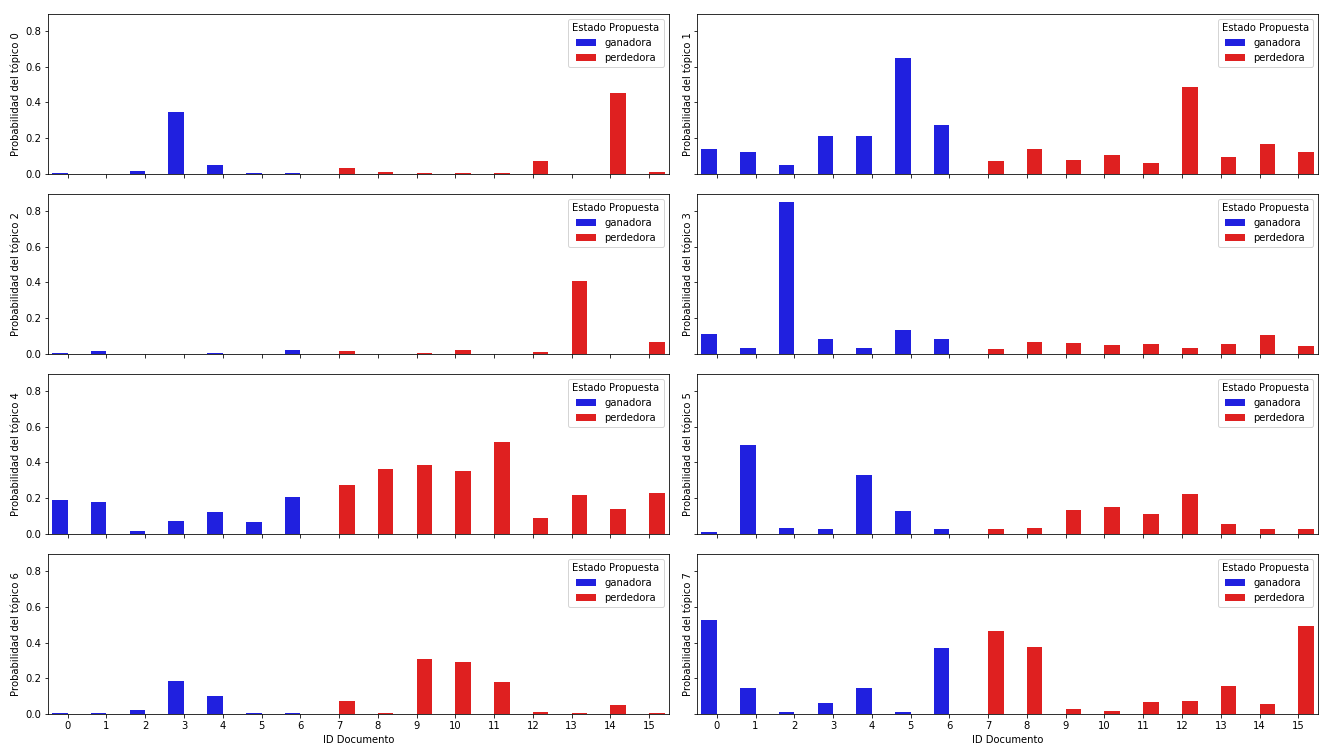
\includegraphics[width=1\textwidth]{figures/LDA/distribution.png}
        \caption{\label{fig:TopicPerDoc} Probabilidad de documentos de pertenecer al tópico $i$} Fuente: Elaboración Propia.
    \end{figure}
    
    Analizando la visualización, se puede apreciar que existen ciertos tópicos que son tratados en sólo ciertos documentos, este es el caso del tópico 2 (\textit{Cobre}) ,por ejemplo, el cual es tratado en un 40\% dentro de un sólo documento y no pasando el 10\% en los documentos restantes.

    Otra cosa interesante que podemos extraer de esta visualización, es que en general todos los documentos tratan algo sobre el tópico 4 llamado Tratamiento de Relaves. De hecho, se puede apreciar que en los documentos perdedores, la importancia para este tópico es superior al 30\%, en 5 de los documentos estudiados. Esto quiere decir, que la mayoría de los documentos perdedores que se han analizado hablan mucho sobre este tema.
    
    Como se sabía del punto anterior los tópicos 3 ``Fundición'' y 2 ``Cobre'', tienen sólo un documento que habla en su mayoría de ellos. Sin embargo, se puede apreciar que el documento que habla más del tópico 3 lo hace en un 80\%. Este documento es probablemente un outlier dentro de la muestra.
    
\paragraph{Clustering usando el resultado de Modelamiento de Tópicos}
    Como se hablo al inicio de esta sección, la distribución de probabilidades de cada documento de pertenecer a cierto tópico puede ser tratada como la identificación de este documento o incluso como features de este mismo. Es por ello que ahora se utilizarán estas características, con el fin de realizar un análisis de clustering.
    
\subparagraph{Distancia entre documentos}
\subparagraph*{}
    En primer lugar, antes de realizar el análisis de clusters, se puede visualizar las distancias entre todos los documentos. Esto sirve, para tener una idea de posibles outliers o clusters que se podrían formar con los datos. Para realizar esto, se decidió utilizar la distancia de Jensen-Shannon , para construir una matriz de distancias entre todos los documentos (Ver figura \ref{fig:DistanceMatrix}). Esta elección se hizo debido a que la distancia de Jensen Shannon, es la única construida para medir distancias entre distribuciones de probabilidades.
    
    \begin{figure}[H]
        \centering
        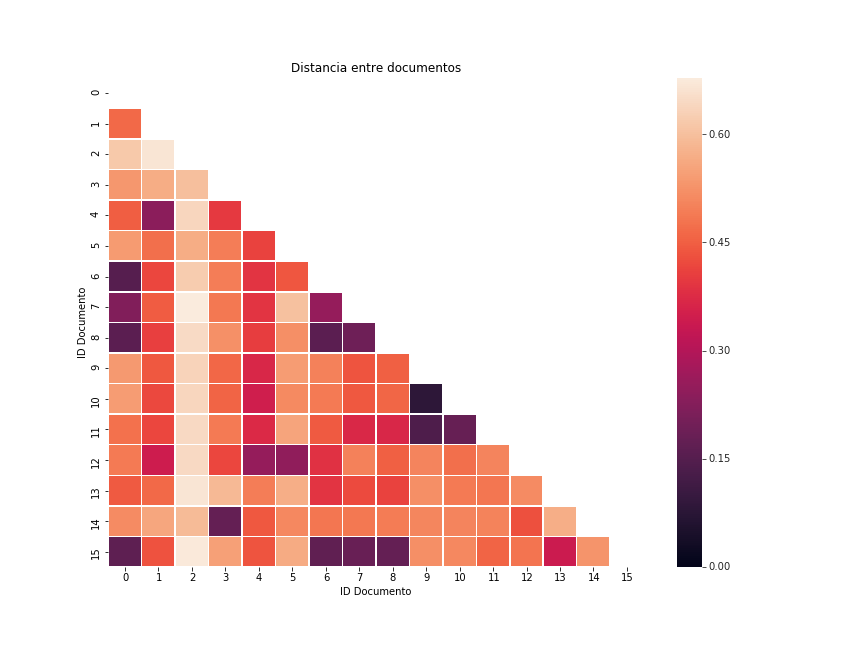
\includegraphics[width=1\textwidth]{figures/Clustering/distancia.png}
        \caption{\label{fig:DistanceMatrix} Matriz de distancia de documentos} Fuente: Elaboración Propia.
    \end{figure}
    
    De esta visualización, se pueden extraer algunas conclusiones:
    \begin{itemize}
        \item El documento 2, es un outlier debido a que se encuentra alejado de todos los documentos. De hecho como habíamos detectado antes, es el único que tiene como tópico principal a ``Fundición''. 
        \item El documento 0, esta muy cercano a los documentos 6,7,8 y 15. Cuyo tópico dominante es Gestión de Cálidad.
    \end{itemize}
    Una vez realizado este análisis, se procederá a aplicar algoritmos de clustering para afirmar las conclusiones recién extraídas.
\subparagraph{Selección del modelo}
\subparagraph*{}
    Para realizar este análisis, se utilizaron dos técnicas de \textit{clustering}: 
    \begin{itemize}
        \item \textbf{K-Means}: Posee como parámetro el número $k$ de \textit{clusters} a encontrar.
        \item \textbf{Jerárquico Aglomerativo}: Posee como parámetros el número $k$ de \textit{clusters} a encontrar, una métrica de distancias y un criterio de enlaces entre \textit{cluster}. 
    \end{itemize}
    Para cada uno de estos algoritmos, se variaron todos sus parámetros construyendo 9 modelos, uno por cada configuración, variando $k$ entre 2 y 9. Para el caso del algoritmo de \textit{clustering} jerárquico aglomerativo se utilizarón las métricas de distancia: Euclidiana, Jensen-Shannon y de Manhattan (Ver sección 2.5.3). Además como criterios de enlace se utilizó: complete, average y single (Ver sección 2.5.3.1). 
    
    Una vez construidos todos los modelos, se procedió a calcular el índice de silhouette para cada uno de ellos (Ver figuras: \ref{fig:aglomerative_silhoutte} y \ref{fig:k-means_silhoutte}). En general se puede apreciar que los mejores resultados se obtienen con $k=7$. De hecho se obtienen los mejores índices de Silhoutte con $k=7$ para k-means y \textit{clustering} aglomerativo con las distancias de manhattan y euclideana usando todos los criterios de enlace.

     \begin{figure}[H]
        \centering
        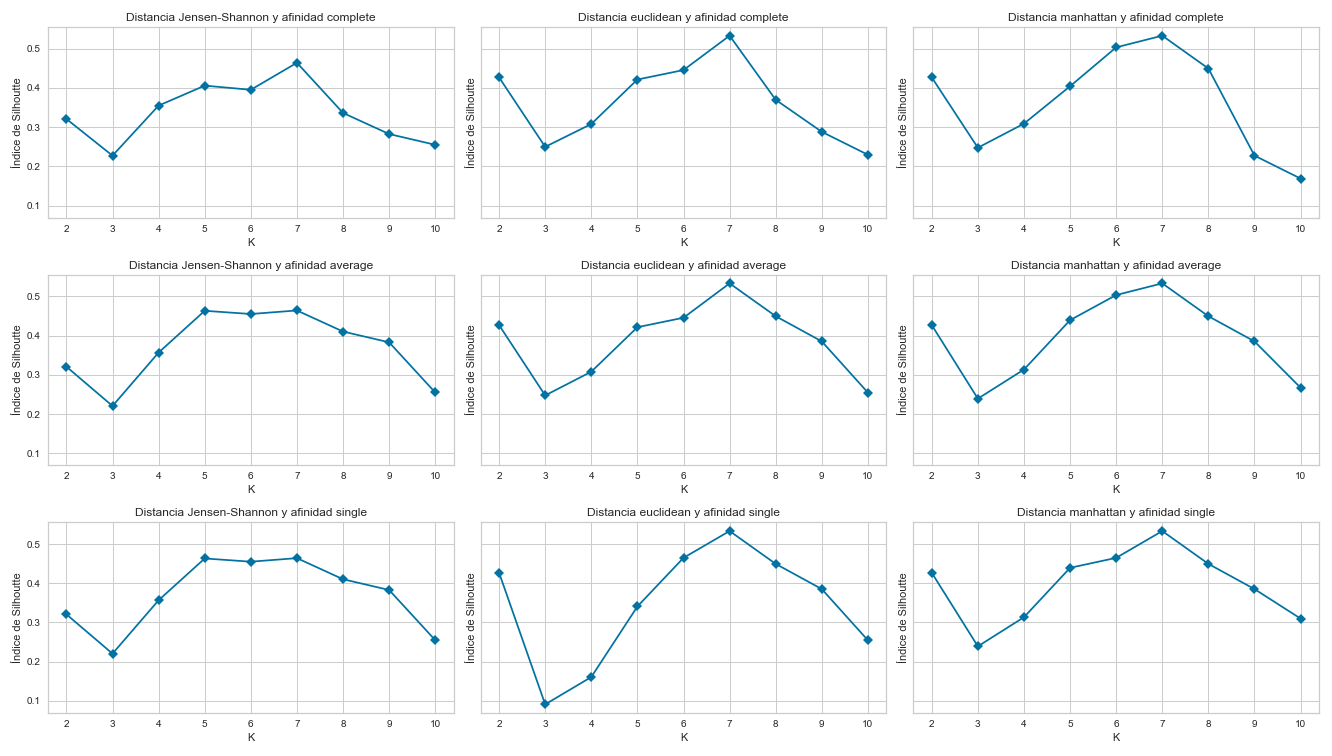
\includegraphics[width=1\textwidth]{figures/Clustering/aglomerative_clustering.png}
        \caption{\label{fig:aglomerative_silhoutte} Evaluación de modelos creados con clustering aglomerativo} Fuente: Elaboración Propia.
    \end{figure}
    
    \begin{figure}[H]
        \centering
        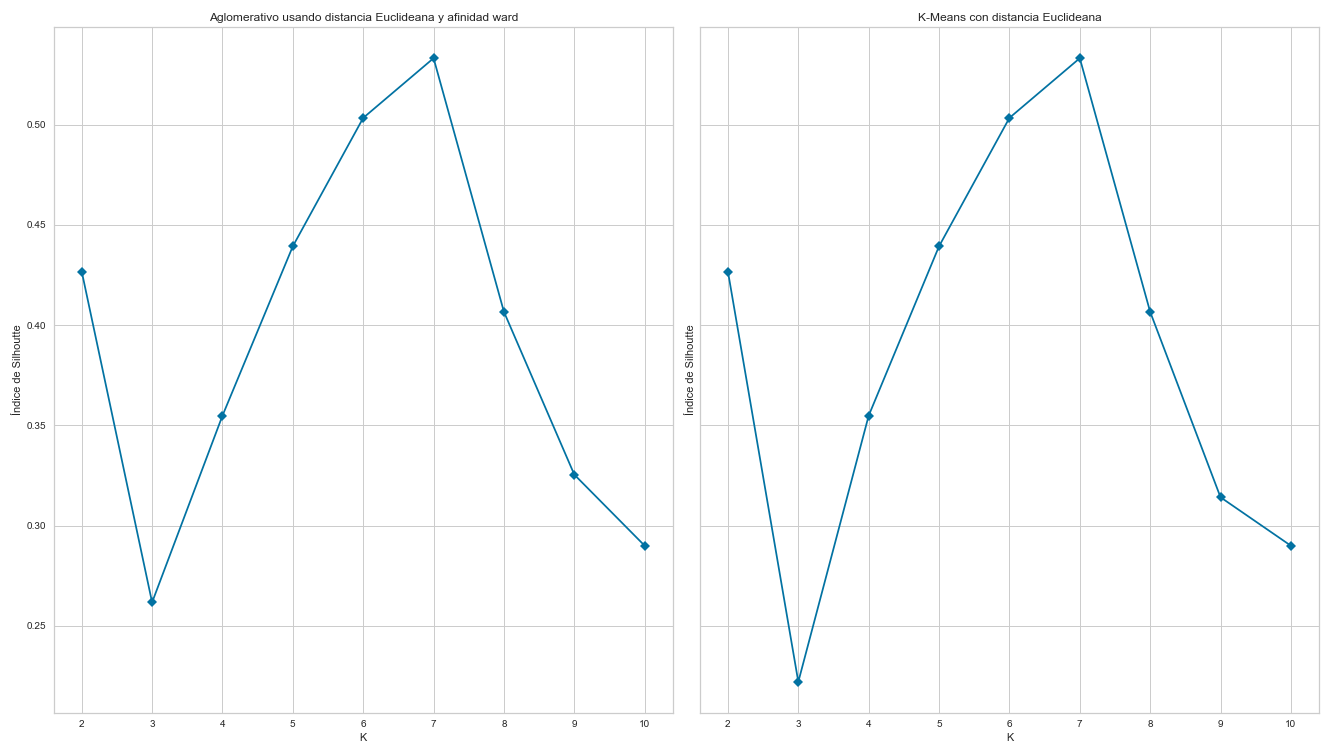
\includegraphics[width=1\textwidth]{figures/Clustering/k-means.png}
        \caption{\label{fig:k-means_silhoutte} Evaluación de modelos creados con clustering aglomerativo y K-Means} Fuente: Elaboración Propia.
    \end{figure}
    
    Considerando lo anterior, se analizó la conformación de los \textit{clusters} con $k=7$ para cada uno de los algoritmos estudiados (Ver tabla: \ref{table:Cluster_Etiquetas}). Como se puede apreciar, los \textit{clusters} encontrados por los dos algoritmos son idénticos a los grupos de temas encontrados por LDA, esto considerando al tópico más relevante como aquel que posee la mayor probabilidad de ocurrencia en el documento. Por ende, pese a que el índice de Silhoutte para la configuración con $k=7$ es el óptimo no consideraremos este modelo. 
    \begin{table}[H]
    \centering
\begin{tabular}{|c|c|c|c|c|}
\hline
   & Tópico más relevante & id Documento & K-Means & Aglomerativo \\ \hline
0  & 7                    & 15-1307      & 2       & 1            \\ \hline
1  & 5                    & 15-3939      & 5       & 2            \\ \hline
2  & 3                    & 14-5143      & 3       & 3            \\ \hline
3  & 0                    & 14-5115      & 4       & 4            \\ \hline
4  & 5                    & 15-4316      & 5       & 2            \\ \hline
5  & 1                    & 15-3732      & 0       & 0            \\ \hline
6  & 7                    & 14-5142      & 2       & 1            \\ \hline
7  & 7                    & 14-5040      & 2       & 1            \\ \hline
8  & 7                    & 14-4984      & 2       & 1            \\ \hline
9  & 4                    & 14-4770      & 1       & 6            \\ \hline
10 & 4                    & 14-5116      & 1       & 6            \\ \hline
11 & 4                    & 14-5205      & 1       & 6            \\ \hline
12 & 1                    & 15-4448      & 0       & 0            \\ \hline
13 & 2                    & 15-4591      & 6       & 5            \\ \hline
14 & 0                    & 15-4400      & 4       & 4            \\ \hline
15 & 7                    & 15-5050      & 2       & 1            \\ \hline
\end{tabular}
    \caption{\label{table:Cluster_Etiquetas} Resumen Etiquetas de documentos para $k=7$} Fuente: Elaboración Propia
\end{table}
    
   Como la configuración utilizada con $k=7$ no fue la deseada, se decidió analizar las configuraciones encontradas para $k=6$ (Ver tabla: \ref{table:Cluster_Etiquetas_6} ) y $k=5$ (Ver tabla: \ref{table:Cluster_Etiquetas_5} ). 
   
   Para el caso de $k=6$, los documentos cuyo tópico dominante es el $7$, ``Gestión de cálidad'', y el $2$, ``Cobre'', se unieron en un único \textit{cluster}. Por otro lado para $k=5$ además del nuevo \textit{cluster}, formado para $k=6$, los documentos cuyo tópico dominante era el $1$, ``Atención al cliente'' y el $5$ ``Construcción'' también se unieron en un único \textit{cluster}.
   
    \begin{table}[H]
    \centering
    \begin{tabular}{|c|c|c|c|}
    \hline
    Tópico más relevante & id Documento & K-Means & Aglomerativo \\ \hline
    0                    & 14-5115      & 4       & 4            \\ \hline
    0                    & 15-4400      & 4       & 4            \\ \hline
    1                    & 15-3732      & 0       & 2            \\ \hline
    1                    & 15-4448      & 0       & 2            \\ \hline
    2                    & 15-4591      & 2       & 0            \\ \hline
    3                    & 14-5143      & 3       & 3            \\ \hline
    4                    & 14-4770      & 1       & 1            \\ \hline
    4                    & 14-5116      & 1       & 1            \\ \hline
    4                    & 14-5205      & 1       & 1            \\ \hline
    5                    & 15-3939      & 5       & 5            \\ \hline
    5                    & 15-4316      & 5       & 5            \\ \hline
    7                    & 15-1307      & 2       & 0            \\ \hline
    7                    & 14-5142      & 2       & 0            \\ \hline
    7                    & 14-5040      & 2       & 0            \\ \hline
    7                    & 14-4984      & 2       & 0            \\ \hline
    7                    & 15-5050      & 2       & 0            \\ \hline
    \end{tabular}
    \caption{\label{table:Cluster_Etiquetas_6} Resumen Etiquetas de documentos para $k=6$} Fuente: Elaboración Propia
    \end{table}
    
    \begin{table}[H]
    \centering
\begin{tabular}{|c|c|c|c|}
\hline
Tópico más relevante & id Documento & K-Means & Aglomerativo \\ \hline
0                    & 14-5115      & 4       & 4            \\ \hline
0                    & 15-4400      & 4       & 4            \\ \hline
1                    & 15-3732      & 0       & 0            \\ \hline
1                    & 15-4448      & 0       & 0            \\ \hline
2                    & 15-4591      & 2       & 2            \\ \hline
3                    & 14-5143      & 3       & 3            \\ \hline
4                    & 14-4770      & 1       & 1            \\ \hline
4                    & 14-5116      & 1       & 1            \\ \hline
4                    & 14-5205      & 1       & 1            \\ \hline
5                    & 15-3939      & 0       & 0            \\ \hline
5                    & 15-4316      & 0       & 0            \\ \hline
7                    & 15-1307      & 2       & 2            \\ \hline
7                    & 14-5142      & 2       & 2            \\ \hline
7                    & 14-5040      & 2       & 2            \\ \hline
7                    & 14-4984      & 2       & 2            \\ \hline
7                    & 15-5050      & 2       & 2            \\ \hline
\end{tabular}
\caption{\label{table:Cluster_Etiquetas_5} Resumen Etiquetas de documentos para $k=5$} Fuente: Elaboración Propia
\end{table}
    Tomando en cuenta todo lo anterior, es que se decidió realizar el análisis para los clusters formados con $k=5$. Esto  debido a que existía una mayor variabilidad en cuanto a la cantidad de tópicos dominantes dentro de un cluster  y además se considera un buen número considerando el número de documentos analizados.
    
\subparagraph{Análisis a cada cluster encontrado}
\subparagraph*{}
    Una vez seleccionada la configuración de \textit{clusters}, se prosiguió a desglozar la composición de cada uno de estos. Para realizar lo anterior, lo primero que se hizo fue revisar que documentos pertenecían a cada uno de los \textit{clusters} encontrados:
    
    \begin{itemize}
        \item El \textit{cluster} número 0 posee los siguientes documentos:
    \begin{itemize}
        \item Documento 0: Licitación 1400000874 ``Estudio de Ingeniería de Cierre Prefactibilidad Explotación Yacimiento Quetenafi ''.
        Esta propuesta fue escrita para el cliente ``Codelco División Chuquicamata ''. Además su tópico más representativo es el 5, Construcción. Finalmente esta propuesta fue ganadora.
        
        \item Documento 1:  ``Servicio de Integridad Estructural Instalaciones Mantención Mina''.
        Esta propuesta fue escrita para el cliente ``Minera Escondida''. Además su tópico más representativo es 5, construcción. Finalmente esta propuesta fue ganadora.
        
        \item Documento 2: ``Licitación CPP-CS-050/15 Servicio de Ingeniería''. Esta propuesta fue escrita para el cliente: ``Codelco Chile División Chuquicamata''. Además su tópico más representativo es 1, Atención al cliente. Finalmente esta propuesta fue ganadora.
        
        \item Documento 3: ``Licitación CPP-CS-044/15 Ingeniería de Detalles Reemplazo Líneas Colectoras y Aducción Inacaliri en Sector Ojos de San Pedro''.
        Esta propuesta fue escrita para el cliente: ``Codelco División Chuquicamat.''- 
        Además su tópico más representativo es 1, Atención al cliente. Finalmente esta propuesta fue perdedora.
    \end{itemize}
    \item El \textit{cluster} número 1 posee los siguientes documentos:
        \begin{itemize}
            \item Documento 0: ``Estudio: Escondida Water Recovery''
            Esta propuesta fue escrita para el cliente: ``Minera Escondida Limitada''. Además su tópico más representativo es 4, Tratamiento de relaves.
            Finalmente esta propuesta fue perdedora.            
            \item Documento 1: ``Estudio Selección Definición Combinada e Ingeniería de Detalles Infraestructura E6''
            Esta propuesta fue escrita para el cliente: ``Minera Escondida''. Además su tópico más representativo es 4, Tratamiento de relaves.
            Esta propuesta fue finalmente : perdedora

            \item Documento 2: ``Integración de Ingenierías de Perfil - Proyecto Crecimiento Modular''.
            Esta propuesta fue escrita para el cliente ``Codelco Chile, División Andina''. Además su tópico más representativo es 4, Tratamiento de relaves. Finalmente esta propuesta fue perdedora.
        \end{itemize}
    \item El \textit{cluster} número 2 posee los siguientes documentos:
        \begin{itemize}
            \item Documento 0: ``Apoyo Restitución Capacidad de Diseño DGM''.
            Esta propuesta fue escrita para el cliente: ``Codelco Chile, División Gabriela Mistral'' 
            Además su tópico más representativo es 7, Control de Cálidad. Finalmente esta propuesta fue ganadora.

            \item Documento 1: ``Ingeniería de Detalles Proyecto Óxidos Encuentro- Planta de Chancado''. Esta propuesta fue escrita para el cliente: ``Antofagasta Minerals S.A''. 
            Además su tópico más representativo es 7, Control de cálidad. Finalmente esta propuesta fue ganadora.
            
            \item Documento 2: ``ODS 23 -  Ingeniería de Detalles Normalización Salas Eléctricas Fundición Caletones Fase I''. Esta propuesta fue escrita para el cliente: ``Codelco División El Teniente''.
            Cuyo Tópico más representativo es 7, Control de calidad. Finalmente esta propuesta fue perdedora.

            \item Documento 3: ``Ingeniería Conceptual Instalación Segundo Picaroca en Chancador Nº1''
            Esta propuesta fue escrita para el cliente: ``Minera Los Pelambres''. 
            Además su tópico más representativo es 7, Control de calidad.
            Finalmente esta propuesta fue perdedora.

            \item Documento 4: ``Licitación VP-FURE-LIC-087 Ingeniería Conceptual Proyecto Desarrollo Fundición Chuquicamata''.
            Esta propuesta fue escrita para el cliente: ``Codelco Chile - Vicepresidencia de Proyectos''. 
            Además su tópico más representativo es 2, Cobre.
            Finalmente esta propuesta fue perdedora.

            \item Documento 5: ``Licitación N  DRT-PRO-3008/15 fiServicio de Ingeniería de Compras para Potenciamiento de Correas 220-CV-204, 220-CV-205, 220-CV-207A y 220-CV-207Bfl''. Esta propuesta fue escrita para el cliente: ``Codelco División Radomiro Tomic''. Además su tópico más representativo es 7, Control de calidad.
            Finalmente esta propuesta fue perdedora.
        \end{itemize}
        \item El \textit{cluster} número 3 posee los siguientes documentos:
        \begin{itemize}
            \item Documento 0: ``Vicepresidencia de Proyectos ICSARA 2 Proyecto Expansión Andina 244 Tranque Ovejería''. Esta propuesta fue escrita para el cliente: ``Codelco Chile''. Además su tópico más representativo es 3, fundición. Finalmente esta propuesta fue ganadora.
        \end{itemize}
        \item El \textit{cluster} número 4 posee los siguientes documentos:
        \begin{itemize}
            \item Documento 0: ``Licitación  Nº 4137/14 - Validación de Capacidad de Diseño Original Depósito de Relaves Filtrados Planta de Tratamiento de Escorias Fundición Potrerillos''. Esta propuesta fue escrita para el cliente: ``Codelco División Salvador''. Además su tópico más representativo es 0, seguridad e impacto ambiental. Finalmente esta propuesta fue ganadora.
            
            \item Documento 1: ``Estudio de Ingeniería Básica y Detalles Conducción Agua Potable El Peñón-Ovalle''. Esta propuesta fue escrita para el cliente: ``Aguas del Valle''. Además su tópico más representativo es 0, Seguridad e impacto ambiental. Finalmente esta propuesta fue perdedora.
        \end{itemize}
    \end{itemize}
    Tomando en cuenta todo lo anterior se puedieron extraer algunas conclusiones sobre cada uno de los \textit{clusters} encontrados. A continuación se detallan algunos de los hallazgos:
    
    \begin{itemize}
        \item \textbf{Cluster 0}: se encuentran 4 documentos de los cuales 3 son escritos para el cliente ``Codelco divisón Chuquicamata''. Por otro lado los tópicos dominantes en este \textit{cluster} son construcción y atención al cliente. Cabe destacar que en las propuestas escritas para el cliente ``Codelco División Chuquicamata'' en dónde el tópico dominante fue atención al cliente la compañía no se adjudico la licitación. Sin embargo en la propuesta en dónde se hablo más sobre construcción si se logró ganar. 
        \item \textbf{Cluster 1}: está compuesto exclusivamente por documentos con el tópico dominante tratamiento de relaves. Por otro lado 2 de los 3 documentos fueron escritos para el cliente ``Minera Escondida''.
        \item \textbf{Cluster 2}: es el \textit{cluster} con mayor número de documentos, 6 para ser exactos. Casi todos los documentos dentro de este clúster poseen como tópico dominante al número 7, Gestión de calidad. Exceptuando un documento que posee como tópico más representativo al tema Cobre. De los documentos que poseen como tópico dominante a Gestión de cálidad, dos resultaron ganadores y fueron escritos para los clientes ``Antofagasta Minerals'' y ``Codelco, División Gabriela Mistral''. El resto de las propuestas en este clúster resultaron perdedoras. 
        \item \textbf{Clúster 3}:  posee un único documento. Este documento puede considerarse como un outlier ya que es el único en la muestra que posee como tópico dominante fundición.
        \item \textbf{Clúster 4}: esta compuesto por 2 documentos cuyo tópico principal es seguridad e impacto ambiental. Uno de estos documentos trata sobre un estudio de Ingeniería básica y de detalles, considerando la estructura del cluster 2 era de esperarse que este documento estuviera en dicho cluster y tuviera como tópico dominante el tema gestión de calidad. Sin embargo no es así por lo que podemos inferir dos cosas: Para el cliente ``Aguas del Valle'' el tema Seguridad e impacto ambiental es más importante que el de gestión de calidad. Si esto no fuera así podemos entregar una connotación negativa a la preponderancia que se le da al tema seguridad e impacto ambiental dentro del documento con respecto a su resultado final, que es perdedor.
    \end{itemize}
    
\subparagraph{Visualización de Clústers}
    Tal como se discutió en el capítulo anterior, la última etapa del experimento de clustering, es poder visualizar los resultados encontrados con el fin de comunicarlos de forma simple. 
    
    En primer lugar, se desarrolló un \textit{scatterplot} usando como técnica de reducción de dimensionalidad a PCA (Ver figura: \ref{fig:PCA}). Dentro de esta visualización, se utilizarón dos elementos para cada punto. El primero, es el uso de círculos para el caso de documentos ganadores y cruces para el caso de documentos perdedores. Por otro lado se pinto de un color distinto a los elementos pertenecientes a distintos clusters.
    
    \begin{figure}[H]
        \centering
        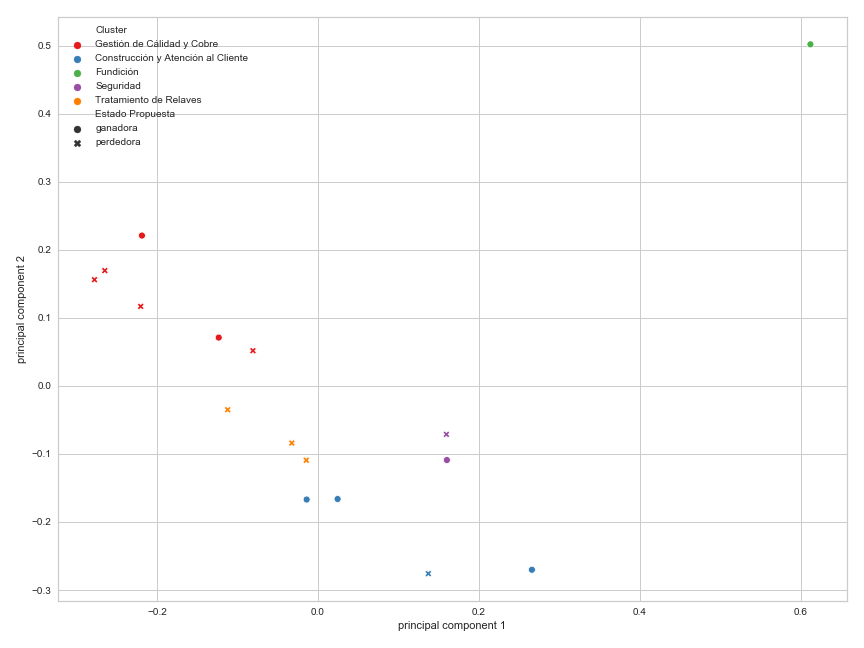
\includegraphics[width=1\textwidth]{figures/Clustering/PCA.png}
        \caption{\label{fig:PCA} Visualización de Clústers usando PCA} Fuente: Elaboración Propia.
    \end{figure}
    
    De la visualización, se pueden apreciar claramente las agrupaciones encontradas en nuestro proceso de clustering. Además nuevamente, se puede ver como el documento que trata sobre Fundición es un outlier dentro de la muestra. 
    
\subsubsection{Opinión de Expertos}
    Una vez terminado todos los experimentos, se procedió a validar los resultados con un experto en el dominio. En nuestro caso se realizó una presentación a la Jefa de Desarrollo de Propuestas, persona lider del equipo encargado de compilar y validar una propuesta antes de ser enviada a los clientes de la compañía.
    
    A continuación se presentan cada uno de los puntos presentados y los respectivos comentarios sobre los resultados obtenidos:
    
    \begin{itemize}
        \item \textbf{Análisis mediante Keywords}:
        \begin{itemize}
            \item Los conceptos comunes a cualquier propuesta detectados por el algoritmo, en general cumplen con los estándares que posee la compañía, por lo que son correctos. Por otro lado los conceptos que destacan en propuestas ganadoras y no en perdedoras, interpretados por el analista como conceptos que podrían ayudar a una propuesta a ganar una licitación,  no entregan información tan valiosa. Esto ocurre ya que el análisis realizado no considera una segregación por clientes y en general las propuestas tienen un estándar distinto para cada uno de estos. Otra segregación interesante que el análisis pasa por alto es el volumen de venta de una propuesta. En general existen distintos niveles de esfuerzo que se le dedican a las propuestas considerando el potencial volumen de venta que estás podrían tener, por lo que repetir el experimento considerando esto también es algo que podría aumentar la calidad de la información detectada.
            
            \item Las conclusiones extraídas para algunos conceptos básicos, detectados por el analista, utilizando análisis de dispersión léxica son correctos en general. Por otro lado se considera a la visualización como una buena herramienta de diagnóstico a una propuesta antes de ser enviada a un cliente. Esto debido a que las propuestas de Hatch hoy en día tienen un formato estandarizado para cada uno de los clientes, por lo que el gráfico de dispersión léxica debería ser el mismo para propuestas escritas para proyectos similares e iguales clientes. 
        \end{itemize}
        \item \textbf{Modelamiento de Tópicos }
        \begin{itemize}
            \item Los temas encontrados en el conjunto de propuestas analizados son correctos. Por otro lado, considerar que uno de los temas más relevantes en las propuestas analizadas es la Gestión de Calidad es coherente con los documentos revisados.
            \item Muchas de las conclusiones extraídas no son generalizables para todas las propuestas.
        \end{itemize}
        \item \textbf{Clustering}
        \begin{itemize}
            \item La información encontrada para el cliente Codelco división Chuquicamata, es considerada información valiosa que no había sido detectada.
        \end{itemize}
    \end{itemize}
    En general, se sugiere repetir los experimentos utilizando una mayor cantidad de datos y realizando los mismos análisis considerando una segregación por clientes y volumen de venta.
\subsubsection{Desarrollo de Guía}
    Considerando todos los patrones encontrados por el analista, más la opinión de los expertos. Se logró generar la siguiente guía de buenas prácticas para la construcción de propuestas técnicas en la compañía.
    \begin{itemize}
        \item Toda propuesta debe poseer al menos un apartado de Gestión de Calidad y otro de Seguridad.
        \item Relacionar los conceptos calidad y Hatch dentro de una misma oración en general tiene una buena acogida por parte de los clientes. Por otro lado, hablar sobre la relación que posee la compañía con los clientes durante el proyecto también es bien recibido.
        \item Se debe intentar hablar sobre las prácticas que posee la compañía sobre ciertos procesos genéricos dentro de un proyecto.
        \item Si la propuesta se está escribiendo para el cliente ``Codelco División Chuquicamata'', en general se debe hablar más sobre los aspectos técnicos de esta por sobre los servicios extras que entrega Hatch tales como Post-Venta.
    \end{itemize}

\newpage
\secnumbersection{CONCLUSIONES}

    En la presente sección, se discuten las principales conclusiones que se obtuvieron una vez finalizado el trabajo.
    
\subsection{Proceso de minería y análisis de textos}
    Durante el desarrollo de esta memoria, se pudo apreciar cómo el uso de técnicas de análisis de textos, puede ser utilizada como una herramienta para la generación de directrices en el diseño de propuestas técnicas de trabajo. Para afirmar lo anterior, se procede a describir las conclusiones que cada uno de los experimentos realizados:
    
    \begin{itemize}
        \item \textbf{Análisis de keywords}: Los patrones que tuvieron un mayor grado de validación por parte del experto en el dominio en esta memoria, fueron los encontrados en este experimento. En general, realizar un análisis mediante \textit{keywords}, no es una tarea muy compleja de realizar. Esto ya que sólo son necesarios conocimientos sobre manejo de Strings y técnicas de conteo. De hecho, a nivel computacional no es costoso y como se comprobó en este trabajo, sus resultados suelen tener una buena aceptación.  Considerando todo lo anterior, se puede concluir que cuando se desea analizar un bajo número de documentos, una buena forma de encontrar patrones útiles es utilizando esta técnica de Análisis de Textos. 
        \item \textbf{Análisis de Dispersión Léxica}: Los patrones encontrados utilizando esta herramienta, también fueron validados por el experto del dominio, por lo que se considera como una herramienta valida a la hora de generar directrices para la generación de propuestas. Por otro lado, el principal desafío a la hora de generar este experimento, fue el desarrollo de la visualización. Esto ya que, las librerías existentes para analizar la dispersión léxica en documentos, sólo permiten realizar análisis para un conjunto de palabras en un único documento. Es por lo anterior que se debió generar desde cero la visualización, diseñada y presentada en la respectiva sección. Finalmente, gracias a la ayuda del experto, también se determinó que esta herramienta puede ser utilizada para entregar un primer diagnóstico a una propuesta en desarrollo.
        
        \item \textbf{Modelamiento de Tópicos}: Si bien el modelamiento de tópicos, es la técnica más compleja que se utilizó en este trabajo, sus resultados no fueron del todo generalizables en relación al objetivo principal de esta memoria. De hecho para el experto, el único patrón relevante encontrado por el uso de esta técnica, es la demostración de que el tema gestión de calidad es importante en los documentos de Hatch. Esto claramente ocurre, ya que el algoritmo utilizado requiere una mayor cantidad de documentos para generar conocimiento algo más útil. Por otro lado, si bien el uso de esta técnica no aportó al objetivo principal de esta memoria, si demostró ser una buena forma de agrupar documentos de forma rápida. Esto puede ser útil en Hatch, debido a que el sistema de gestión de documentos que actualmente utiliza la compañía, no posee ningún mecanismo para la extracción inteligente de los datos. Es decir, realizar extracciones por fecha, cliente o dominio del proyecto. Por ende, estos deben ser extraídos de forma manual y si se quisieran realizar agrupaciones de éstos, también deben hacerse de la misma forma.
        
        \item \textbf{Clustering de documentos}: El experimento de \textit{clustering} de documentos, utilizando los resultados de modelamiento de tópicos, en general tuvo resultados positivos siendo el más útil el patrón encontrado para el cliente ''Codelco División Chuquicamata``. La implementación de este experimento no fue de gran complicación y en general los resultados tienen un costo computacional bajo en términos de tiempos de ejecución. Sin embargo, la tarea más compleja a la hora de realizar un análisis mediante \textit{clustering}, es la caracterización de los clústers encontrados. Esto ya que como se quiere caracterizar un conjunto de documentos, además de analizar el texto en sí, se debe extraer la metada asociado a este (Nombre del proyecto y cliente en nuestro caso). Esto, con el fin de poder interpretar utilizando la mayor cantidad de información las agrupaciones encontradas por el algoritmo.
    \end{itemize}

\subsection{Resultados}
    En general, se lograron encontrar varios patrones en propuestas que habían sido declaradas ganadoras en sus respectivas licitaciones. Si bien, no todos estos patrones fueron validados por el experto en el dominio para ser agregados al producto final de esta memoria, si se valora la automatización y generalización de los experimentos para ser repetidos en un conjunto de datos más grande que el utilizado en este trabajo. Esto, con el fin de encontrar patrones con un mayor grado de confiabilidad y además más precisos.
    
    Por otro lado, la no aprobación de muchos de los patrones encontrados en este trabajo, se debe más que nada a la poca cantidad de datos analizados. Esto, ya que mucha de la información extraída tenía poca capacidad de ser generalizada, debido a que aparecía en un número ínfimo de propuestas.
    
    Finalmente, también se encontró como ciertas visualizaciones podían ser utilizadas como herramientas de diagnóstico durante el proceso de producción de una propuesta. Este fue el caso del gráfico de dispersión léxica, el cual puede entregar  un diagnóstico sobre si una propuesta está cumpliendo o no la estructura básica de una propuesta Hatch. Por ejemplo en nuestra guía, se nombró que toda propuesta en Hatch debe tener una sección de Gestión de calidad y otra de Seguridad, por lo que utilizando este gráfico se hace sencillo y rápido verificar el cumplimiento de esto.

\subsection{Dificultades a la hora de desarrollar el trabajo}
    Dentro del desarrollo de este trabajo, se presentaron algunos inconvenientes que se describen a continuación:
    \begin{itemize}
        \item \textbf{Extracción de datos}: Dentro de la compañía, si bien existe un sistema de gestión de documentos, éste no es más que un gestor de archivos. Es por ello, que la extracción de datos es sumamente lenta y se debe realizar de forma manual. Por otro lado, el acceso a estos documentos es sumamente restringido dentro de la compañía, por lo que acceder a dicho sistema requiere de ciertos privilegios que el autor de este documento no poseía. Es por lo anterior, que para obtener los documentos que fueron analizados en esta memoria se requirió ayuda de personal de la compañía. El problema aquí es que por ejemplo si se requiere obtener todos los documentos que fueron escritos para un cierto cliente $X$, se deben solicitar a alguna persona con los privilegios para acceder a esa información. Luego, dicha persona debe buscar uno a uno dentro del directorio los archivos que cumplan con la restricción solicitada. Es por lo anterior que el proceso de extracción de datos dentro de la compañía es sumamente lento. Para mejorar esto, es que se recomienda tener un sistema de bases de datos que permita extraer los documentos de una manera más rápida por las personas que tengan acceso a dichos documentos.
        \item \textbf{Pocas librerías de procesamiento de lenguaje natural en español}: Otra dificultad que se encontró al desarrollar este trabajo, es el poco desarrollo de liberías de procesamiento de lenguaje natural adaptadas al español. Por ejemplo, en el marco conceptual se explicaron conceptos como: Stemming, Lematización y Part of Speech. En general si bien hay librerías que realizan estas tareas básicas de procesamiento de lenguaje natural, la mayoría lo hace de forma bastante defectuosa para textos en español. Esto ocurre sobre todo a la hora de manejar conceptos técnicos, como es nuestro caso. Es por ello que cuando se diseñaron los experimentos, se decidió dejar de lado el uso de estas tareas en nuestro preprocesador de textos.
        \item \textbf{Sensibilidad con respecto al uso de datos}: Uno de los principales problemas que se tuvo durante el desarrollo de esta memoria, fue el rechazo y preocupación de ciertos directivos dentro de la compañía al percatarse que una persona externa a la organización estaba explorando las propuestas. Esto trajo problemas, ya que luego de esto, se disminuyó la cantidad de datos a analizar y por ende disminuyó la calidad de los resultados del trabajo. De esta experiencia, se puede ver que para ejecutar un proyecto de análisis y minería de textos, con datos sensibles como lo son las propuestas de una empresa, se debe conseguir el apoyo de todos los Stakeholders del proyecto antes de realizar cualquier análisis. Esto con el fin de asegurar el transcurso normal del proyecto.
        \item \textbf{Poco conocimiento en análisis de textos por parte del analista}: Otro problema que se debió resolver a medida que se desarrollaba esta memoria, fue el nulo conocimiento de análisis de textos por parte del autor antes de enfrentar el desafío impuesto por la memoria. Es por ello, que mucho del tiempo invertido en el desarrollo de este trabajo fue dedicado principalmente, al estudio sobre técnicas de análisis y minería de textos. 
        
    \end{itemize}

\subsection{Trabajo futuro}
    A partir del desarrollo de esta memoria, es claro que los patrones encontrados pudieron haber tenido una calidad superior. Es por ello que como trabajo futuro, se recomienda repetir los experimentos realizados en este trabajo pero esta vez, utilizando las recomendaciones del experto. Es decir, se deben repetir los experimentos utilizando una mayor cantidad de documentos y realizar análisis separados por clientes y volumen de venta de cada propuesta. 
    
    Por otro lado, como se mencionó anteriormente, otro problema detectado en esta memoria fue la forma en que se almacenaban las propuestas dentro de la compañía. Considerando el volumen de documentos almacenados por la compañía y la idea de realizar análisis de manera sostenida y continúa de aquí en mas, es que se hace insostenible seguir con el sistema actual, por ende se propone reemplazarlo por alguna base de datos más moderna. Esto debido a que la extracción de los datos utilizando el sistema actual se debe realizar de forma manual, haciendo el proceso lento y tedioso para la persona encargada de ejecutarlo. Por otro lado, dicha persona se puede transformar en un cuello de botella dentro del proyecto haciendo más larga la duración de este. 

\subsection{Conclusiones finales}
    En base a todos los experimentos efectuados sobre el conjunto de documentos analizados, es posible concluir que efectivamente este tipo de datos es apto para ser analizados utilizando técnicas de análisis de textos. De hecho, ciertos experimentos demostraron ser potenciales herramientas para realizar análisis de forma más eficiente a la estructura de una propuesta (análisis de dispersión léxica), mejorando el proceso de diagnóstico actual que se realiza en la compañía. Además realizando los experimentos con un número ínfimo de datos, se lograron encontrar algunos patrones, que no habían sido detectados, utilizando los métodos manuales que se efectúa hasta la fecha en la compañía. Por lo anterior se presume que escalar estos experimentos definitivamente entregarán mejores patrones y ayudarán a generar mejores directrices para el desarrollo de nuevas propuestas.





\newpage
% Bibliografía estilo APA:
\bibliographystyle{apalike-es}
\bibliography{bibliografia}{}

\newpage
\input{anexos}

\end{document}
